\documentclass[11pt,a4paper]{article}
\usepackage{algorithm, algorithmic, listings} % Code
\usepackage{amsmath,mathtools,amssymb,amsfonts,dsfont,cancel} % Math
\usepackage{amstext}
\usepackage{color, xcolor} % Color
\usepackage{diagbox, tabularx} % Table
\usepackage{enumerate} % List
\usepackage{epsfig, epstopdf, graphicx, multicol, multirow, palatino, pgfplots, subcaption, tikz} % Image.
\usepackage{fancybox}
\usepackage{verbatim}

\usepackage[margin=1in]{geometry}
\usepackage[hidelinks]{hyperref}
\epstopdfsetup{outdir=./Figure/Converted/}
\graphicspath{{./Figure/}{./Figure/part_ii_q_3}{./Figure/part_ii_q_4}{./Figure/part_iii_q_3}}
\pgfplotsset{compat=1.13}

% MATLAB
\lstset{extendedchars=false, basicstyle=\normalsize\tt, language=Matlab, tabsize=4, numbers=left, numberstyle=\small, stepnumber=1, numbersep=8pt, keywordstyle=\color[rgb]{0,0,1}, commentstyle=\color[rgb]{0.133,0.545,0.133}, stringstyle=\color[rgb]{0.627,0.126,0.941}, backgroundcolor=\color{white}, showspaces=false, showstringspaces=false, showtabs=false, frame=single, captionpos=t, breaklines=true, breakatwhitespace=false, morekeywords={break, case, catch, continue, elseif, else, end, for, function, global, if, otherwise, persistent, return, switch, try, while}, title=\lstname,
mathescape=true,escapechar=? % escape to latex with ?..?  
escapeinside={\%*}{*)}, % if you want to add a comment within your code  
%morestring=[m]', % strings
%columns=fixed, % nice spacing
}

\begin{document}
\title{\sc\vspace{3cm}\hrule\vspace{0.3cm}{\LARGE EL2320}\\\vspace{0.1cm}{\Large Applied Estimation}\vspace{0.3cm}\hrule\vspace{1.5cm}{\Large Laboratory Report}\\{\large Lab 2: Particle Filter}}
%\title{\LARGE{\sc{EL2320 Applied Estimation}}\\\Large{Lab 2: Particle Filter}}
\author{Jiang, Sifan\\{\small sifanj@kth.se}}
\maketitle
\newpage

\newcounter{Counter}
\setcounter{Counter}{0}
\section{Introduction}
\par \textbf{Particle Filters:}
\begin{enumerate}
	\item What are the particles of the particle filter?
		\par Particles are also called samples. They are used to represent the posterior distribution of some stochastic process given noisy.

	\item What are importance weights, target distribution, and proposal distribution and what is the relation between them?
		\begin{itemize}
			\item Importance wights $w_t^{[m]}$ is the probability of a measurement $z_t$ regarding a particle $x_t^{[m]}$. So that $w_t^{[m]} = p(z_t | x_t^{[m]})$.
			\item Target distribution represents the belief $bel(x_t)$. 
			\item Proposal distribution represents the $\overline{bel}(x_t)$ based on the prior belief over state $x_{t-1}$ and the control $u_{t}$.
		\end{itemize}
		\par Target distribution can be sampled from the proposal distribution. Each sample could be drawn with a probability equals to importance weight.

	\item What is the cause of particle deprivation and what is the danger?
		\par The cause of particle deprivation is the lack of particles which could be caused by re-sampling. The danger of particle deprivation is that there would be no particles around the true state of the system.

	\item Why do we re-sample instead of simply maintaining a weight for each particle always.
		\par Without re-sampling most particles would represent states with a low likelihood after some time and the filter would loose track of the ``good'' hypotheses.

	\item Give some examples of the situations which the average of the particle set is not a good representation of the particle set.
		\par When the posterior is multi-modal, the average of the particle set would be not good for representing the multiple regions of true interest.

	\item How can we make inferences about states that lie between particles.
		\par Inferences about states that lie between particles can be made by histograms, where the bin is set by adjacent particles, or Gaussian kernels where each particle is used as the center of a Gaussian kernel.

	\item How can sample variance cause problems and what are two remedies?
		\par High sample variance can cause incorrect estimation about the true state.
		\par Remedies:
		\begin{itemize}
			\item Reducing the re-sampling frequency.
			\item Using a sequential stochastic process instead.
		\end{itemize}

	\item For robot localization for a given quality of posterior approximation, how are the pose uncertainty (spread of the true posteriori) and number of particles we chose to use related.
		\par Higher pose uncertainty would result in larger spread of the posteriori, so, larger number of particles are needed. 
\end{enumerate}

\setcounter{Counter}{0}
\section{Warm up problem with the Particle Filter}
\subsection{Prediction}
\begin{itemize}
	\item\addtocounter{Counter}{1}\textbf{Question \arabic{Counter}:} What are the advantages/drawbacks of using (6) compared to (8)? Motivate.
		\par In section 2D State Space, (6) uses the same value of angle $\theta_{0}$ for all time steps. This equation will give precise prediction when target moving on a line if there is no noise or diffusion. Also, same value for angle could improve computational time. However, since there is noise in the system, the estimate of the motion will result in a wave-like pattern. In section 3D State Space, (8) uses the angle obtained from the previous time stamp to replace the fixed angle, the estimate of the motion will result in a smoother line compared to what (6) gives.

	\item\addtocounter{Counter}{1}\textbf{Question \arabic{Counter}:} What types of circular motions can we model using (9)? What are the limitations (what do we need to know/fix in advance)?
		\par We need to know the initial velocity $v_{0}$ and $\omega_{0}$ to determine what exactly the type of circular motion would (9) modeled. Equation (9) could model any circular motion with angular velocity based on the previous time stamp.
\end{itemize}

\subsection{Sensor Model}
\begin{itemize}
	\item\addtocounter{Counter}{1}\textbf{Question \arabic{Counter}:} What is the purpose of keeping the constant part in the denominator of (10)?
		\par The purpose of keeping the constant part in the denominator of Equation (10) is to make the integral over the whole distribution to be $1.0$ making the likelihood function for the observation a probability distribution.
\end{itemize}

\subsection{Re-Sampling}
\begin{itemize}
	\item\addtocounter{Counter}{1}\textbf{Question \arabic{Counter}:} How many random numbers do you need to generate for the Multinomial re-sampling method? How many do you need for the Systematic re-sampling method?
		\par Based on the algorithms, we need $M$ random number for the Multinomial re-sampling method where $M$ is the number of . And we need only $1$ random number for the Systematic re-sampling.

	\item\addtocounter{Counter}{1}\textbf{Question \arabic{Counter}:} With what probability does a particle with weight $\omega = \frac{1}{M} + \epsilon$  survive the re-sampling step in each type of re-sampling (vanilla and systematic)? What is this probability for a particle with $0 \leq \omega < \frac{1}{M}$? What does this tell you? (Hint: it is easier to reason about the probability of not surviving, that is M failed binary selections for vanilla, and then subtract that amount from $1.0$ to find the probability of surviving.
		\par In the Multinomial re-sampling, for each particle $p^{[k]}$, there is a probability of $\omega^{[k]}$ to be selected in one iteration. The probability of being chosen is equal to its importance weight. So, the probability of not being selected for particle $p^{[k]}$ would be $1 - \omega^{[k]}$. So, the probability for a certain particle of not being selected for $N$ iterations would be $(1 - \omega^{[k]})^{N}$, thus, the probability of surviving the re-sampling would be $1 - (1 - \omega^{[k]})^{N}$.
		\par In the Systematic re-sampling, particles $p^{[k]}$ with importance weight $\omega^{[k]} = \frac{1}{M} + \epsilon$ where $\epsilon \in (0, 1]$, would always be selected since the selection step size $\frac{1}{M} < \frac{1}{M} + \epsilon$. If the importance weight $\omega^{[k]} \in \left[ 0, \frac{1}{M} \right)$, the probability of surviving would be $M \omega^{[k]}$. The random number $r_{0}$ is uniformly distributed over $\left[ 0, \frac{1}{M} \right]$, also the probability of selection of a particle is proportional to its weight, the probability of surviving the re-sampling would be $M \omega^{[k]}$.
\end{itemize}

\subsection{Experiments}
\begin{itemize}
	\item\addtocounter{Counter}{1}\textbf{Question \arabic{Counter}:} Which variables model the measurement noise/process noise models?
		\par Variable \texttt{Sigma\_Q} model the measurement noise model.
		\par Variable \texttt{Sigma\_R} model the process noise model.

	\item\addtocounter{Counter}{1}\textbf{Question \arabic{Counter}:} What happens when you do not perform the diffusion step? (You can set the process noise to 0)
		\par If the process noise is set to $0$, according to equation (3), the predicted state would be equal to applying motion. Also, for a fixed target, $\overline{u}_{t} = 0$ for all time stamps, thus $\overline{x}^{m}_{t} = x_{t-1}^{m}$. So, it's predictable that the result would be $M$ copies of the same particle.

	\item\addtocounter{Counter}{1}\textbf{Question \arabic{Counter}:} What happens when you do not re-sample? (set RESAMPLE\_MODE=0)
		\par If not re-sampling the particles, then all the particles would be remained no matter how much the importance weight. The motion of each particle simulates the estimation of the true state from a different initial state and no convergence would be obtained. As a result, the particles would spread over the whole region and with large estimation error.

	\item\addtocounter{Counter}{1}\textbf{Question \arabic{Counter}:} What happens when you increase/decrease the standard deviations (diagonal elements of the covariance matrix) of the observation noise model? (Try values between 0.0001 and 10000)
		\par When increasing the standard deviations of the observation noise model from 0.0001 to 10000, the expectation to the accuracy of the estimation of the measurements is decreasing. If the standard deviations is small, then the estimates would not likely to be close to the true measurements, thus being regarded as outliers. So the estimate would hard to converge to the true state.
		\par When the standard deviations is big, then the estimates are easy to follow the true measurements closely, thus the estimate would easy to converge to the true state but with big variance and uncertainty.

	\item\addtocounter{Counter}{1}\textbf{Question \arabic{Counter}:} What happens when you increase/decrease the standard deviations (diagonal elements of the covariance matrix) of the process noise model? (Try values between 0.0001 and 10000)
		\par When increasing the standard deviations of the process noise model, the diversity of the particle population is also increasing. When the deviation is small, the cluster of particles around the true state is also small and condensed in a certain region but with no guarantee to convergence. When the deviation is big, the particles spread around the true state and have a relatively big radius of the cluster.

	\item\addtocounter{Counter}{1}\textbf{Question \arabic{Counter}:} How does the choice of the motion model affect a reasonable choice of process noise model?
		\par If the motion model is accurate to describe the true state, then the process noise can be small. If the motion model is known to be not accurate to model the true motion, the process noise should be large enough for particles to be able to estimate the true motion.

	\item\addtocounter{Counter}{1}\textbf{Question \arabic{Counter}:} How does the choice of the motion model affect the precision/accuracy of the results? How does it change the number of particles you need?
		\par If a motion model model the actual motion accurately, then the results would also be precise and accurate. As a result, small number of particles would be needed because of the high accuracy of the particles. While larger number of particles would be needed for less accurate model so that the system could converge to true state.

	\item\addtocounter{Counter}{1}\textbf{Question \arabic{Counter}:} What do you think you can do to detect the outliers in third type of measurements? Hint: what happens to the likelihoods of the observation when it is far away from what the filter has predicted?
		\par We can introduce a threshold value for the likelihoods of the observation. When the measurement is far away from what the filter has predicted, the likelihood of this observation would be very small and could be smaller than the threshold. So, in this way, outliers could be detected and removed in third type of measurements.

	\item\addtocounter{Counter}{1}\textbf{Question \arabic{Counter}:} Using 1000 particles, what is the best precision you get for the second type of measurements of the object moving on the circle when modeling a fixed, a linear or a circular motion(using the best parameter setting)? How sensitive is the filter to the correct choice of the parameters for each type of motion?
		\par Change the function: \texttt{pf\_track(Z, X, VERBOSE, Dimension, Motion, Sigma\_Q, Sigma\_R)}, so that we can easily change the parameters.
		\begin{itemize}
			\item \texttt{Z}, the measurement of the object, is \texttt{circ\_meas\_2}.
			\item \texttt{X}, the ground true information, is \texttt{circ\_true}.
			\item \texttt{Dimension} is $3$.
			\item \texttt{Sigma\_Q}, the measurement noise covariance matrix, is chosen from 5 values: 100, 250, 500, 750, and 1000. 
			\item \texttt{Sigma\_R}, the prediction noise covariance matrix, is chose from 5 values: 1, 10, 25, 50, 75, and 100.
		\end{itemize}
		\par In all I would try 25 pairs of noises and from which I could obtain the best parameter setting so that having the minimized error.
		\par When \texttt{Motion} is $0$ which means modeling a fixed motion, we have following noises so that the error is $11.3 \pm 5.4$. It is very sensitive to the correct choice of the parameters and requires high level of process noise in order for the particles to be able to follow the true state.
		\begin{align*}
			R &= \begin{bmatrix} 25 & 0 & 0 \\ 0 & 25 & 0 \\ 0 & 0 & 0.01 \end{bmatrix} \\
			Q &= \begin{bmatrix} 500 & 0 \\ 0 & 500 \end{bmatrix}
		\end{align*}
		\par When \texttt{Motion} is $1$ which means modeling a linear motion, we have following noises so that the error is $7.5 \pm 3.5$. It is not very sensitive to the correct choice of the parameters.
		\begin{align*}
			R &= \begin{bmatrix} 1 & 0 & 0 \\ 0 & 1 & 0 \\ 0 & 0 & 0.01 \end{bmatrix} \\
			Q &= \begin{bmatrix} 250 & 0 \\ 0 & 250 \end{bmatrix}
		\end{align*}
		\par When \texttt{Motion} is $2$ which means modeling a circular motion, we have following noises so that the error is $7.2 \pm 3.3$. It is not sensitive to the correct choice of the parameters and allows low level noise to converge to true state.
		\begin{align*}
			R &= \begin{bmatrix} 1 & 0 & 0 \\ 0 & 1 & 0 \\ 0 & 0 & 0.01 \end{bmatrix} \\
			Q &= \begin{bmatrix} 250 & 0 \\ 0 & 250 \end{bmatrix}
		\end{align*}
\end{itemize}

\section{Main Problem: Monte Carlo Localization}
\begin{itemize}
	\item\addtocounter{Counter}{1}\textbf{Question \arabic{Counter}:} What parameters affect the mentioned outlier detection approach? What will be the result of the mentioned method if you model a very weak measurement noise $|Q| \rightarrow 0$?
		\par The threshold $\lambda_{\Psi}$ affects the mentioned outlier detection approach. The higher the value of $\lambda_{\Psi}$ is, the easier for a particle to be an outlier. Also, the measurement noise $Q$ would also have effect on the detection. If the noise is very weak so that $|Q| \rightarrow 0$, the confidence in the measurement result would be very high and the tolerance between the difference between the prediction and true value decreases, thus making more measurements are regarded as outliers. 

	\item\addtocounter{Counter}{1}\textbf{Question \arabic{Counter}:} What happens to the weight of the particles if you do not detect outliers?
		\par If not detecting outliers, then all the measurements are considered to be valid so the measurements would be equally trusted. And because the wrong measurements would be taken into consideration, the weights of the particles would also be wrong.
\end{itemize}

\subsection{Data Sets}
\subsubsection{map\_sym2.txt + so\_sym2\_nk}
\par \texttt{part\_bound} would have influence on the initial position of each particles in the global localization. According to the code, we would have the initial $x$ and $y$ coordinates for the particles:
	\begin{align}
		S(1,:) &= rand(1,M) * [ bound(2) - bound(1) + 2 * part\_bound ] + bound(1) - part\_bound \\
		S(2,:) &= rand(1,M) * [ bound(4) - bound(3) + 2 * part\_bound ] + bound(3) - part\_bound
	\end{align}
So, the higher the value of \texttt{part\_bound} is, the more likely for the particles to spread out to a bigger region, thus the particles are easier to be distinguished from each and kept as reliable hypotheses.

\begin{figure}[]
	\centering
	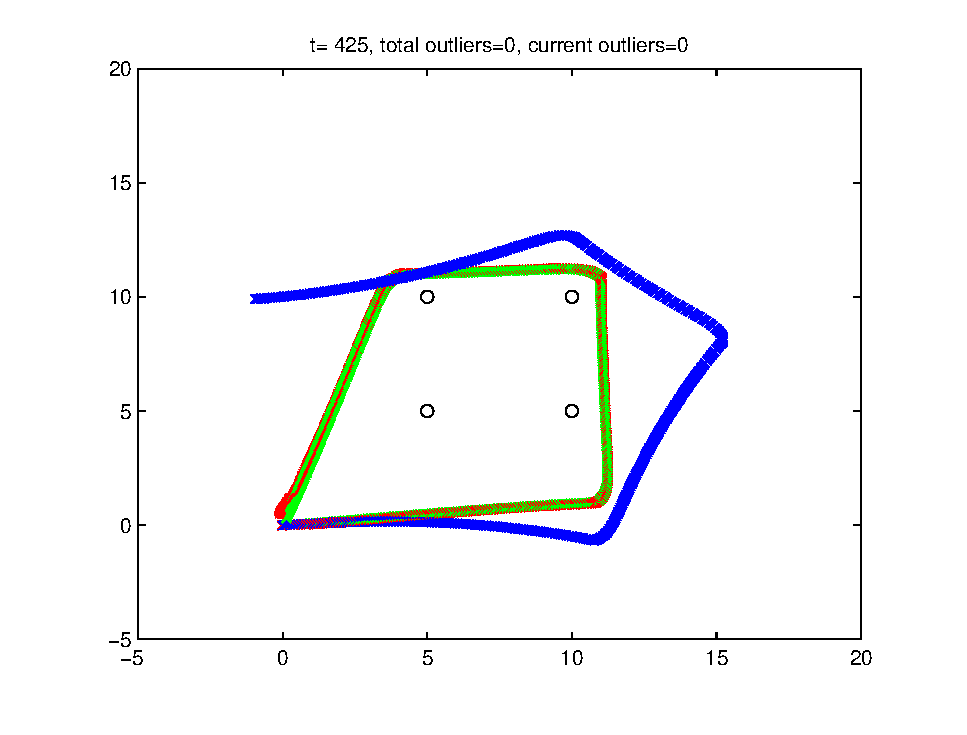
\includegraphics[scale=0.5]{Tracking_Trajectory_Map_2_M_1000.eps}
	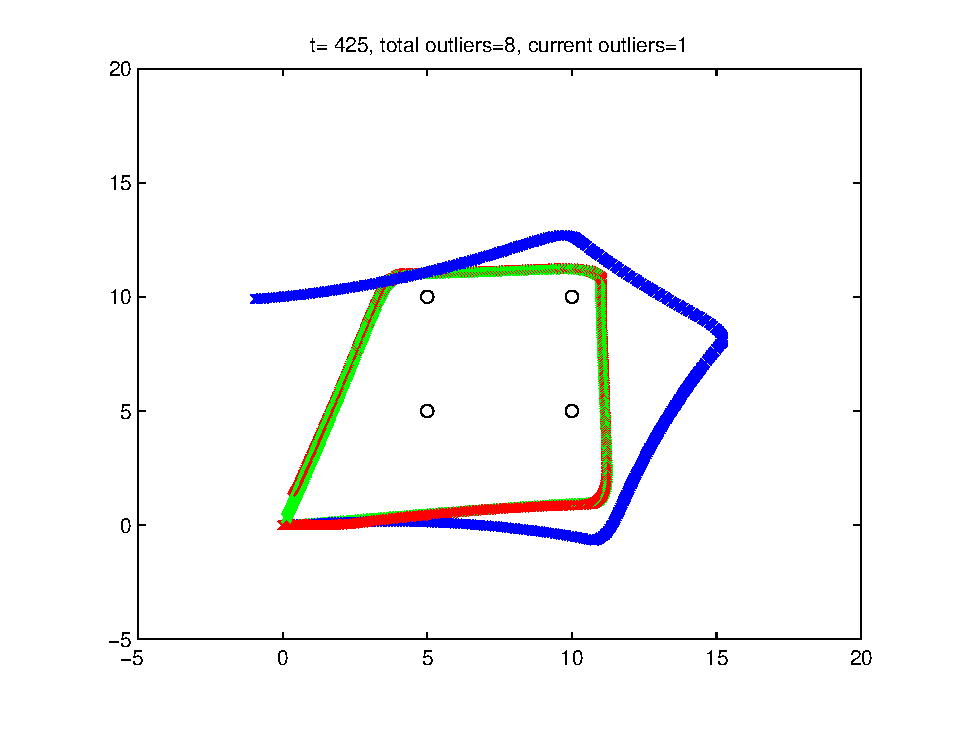
\includegraphics[scale=0.5]{Tracking_Trajectory_Map_2_M_10000.eps}
	\caption{Result when the number of particles $M=1000$ (left) and $M=10000$ (right).}
	\label{fig:Tracking_Map_2_M_1000_10000}
\end{figure}

\begin{figure}
	\centering
	\scalebox{0.5}{% This file was created by matlab2tikz.
%
%The latest updates can be retrieved from
%  http://www.mathworks.com/matlabcentral/fileexchange/22022-matlab2tikz-matlab2tikz
%where you can also make suggestions and rate matlab2tikz.
%
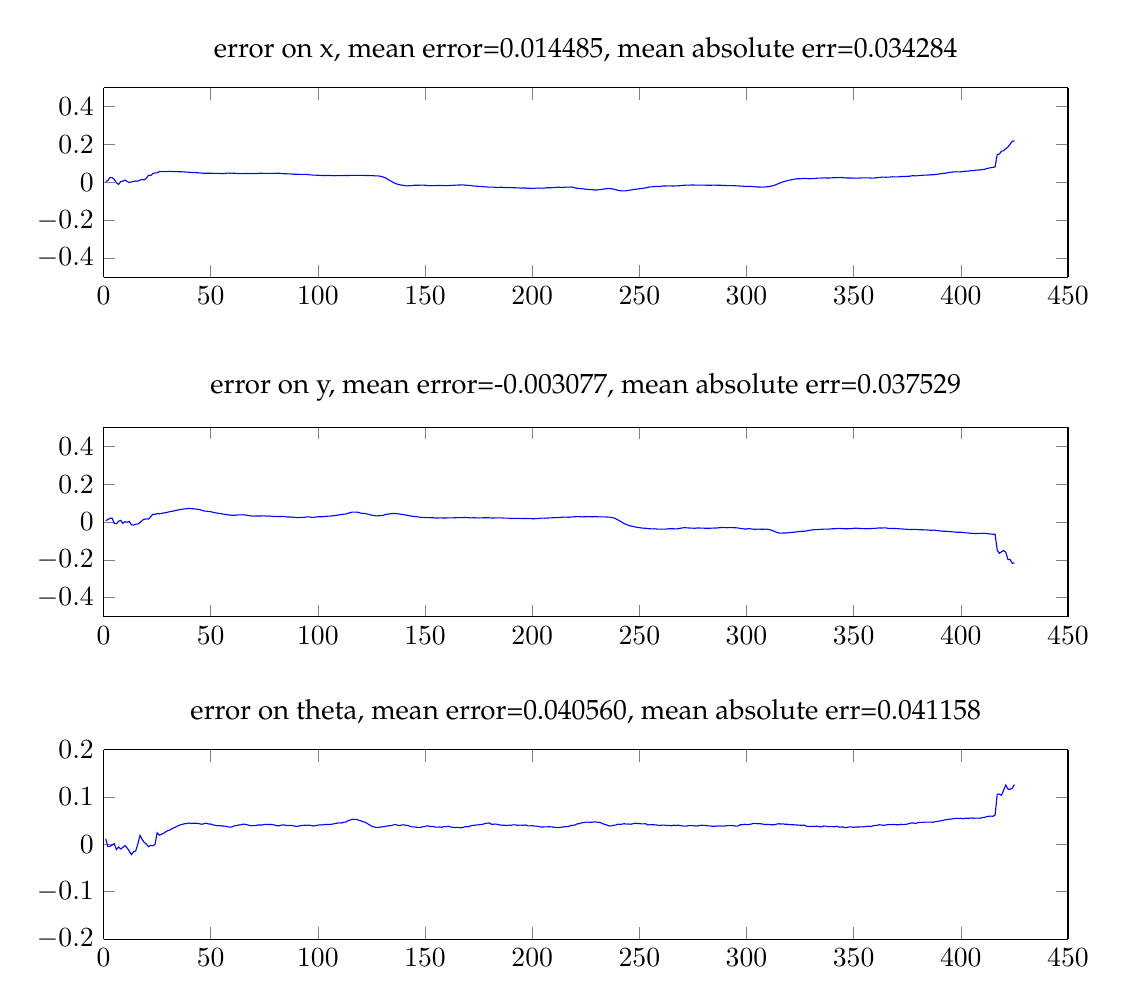
\begin{tikzpicture}

\begin{axis}[%
width=4.822in,
height=0.947in,
at={(0.809in,3.31in)},
scale only axis,
separate axis lines,
every outer x axis line/.append style={black},
every x tick label/.append style={font=\color{black}},
xmin=0,
xmax=450,
every outer y axis line/.append style={black},
every y tick label/.append style={font=\color{black}},
ymin=-0.5,
ymax=0.5,
axis background/.style={fill=white},
title={error on x, mean error=0.014485, mean absolute err=0.034284}
]
\addplot [color=blue,solid,forget plot]
  table[row sep=crcr]{%
1	0.00496604804055681\\
2	0.00962950903304788\\
3	0.0262500946491253\\
4	0.0250473906908557\\
5	0.0156176743994615\\
6	-0.00192493295636949\\
7	-0.0103699480315349\\
8	0.00432522941514643\\
9	0.00673932308003251\\
10	0.0122917704611131\\
11	0.00500443416404532\\
12	-0.000579239775318438\\
13	0.00239930999274323\\
14	0.0049746212525062\\
15	0.0076179103941427\\
16	0.00648657693858989\\
17	0.0123697001603848\\
18	0.0155720875622895\\
19	0.0130450385675461\\
20	0.0229025177775352\\
21	0.0379717004827652\\
22	0.0362896427219375\\
23	0.0464927152333016\\
24	0.0504194024826177\\
25	0.0501390712204925\\
26	0.057595800863546\\
27	0.0570463790087716\\
28	0.0571532774395651\\
29	0.0570379602255484\\
30	0.0579156773930254\\
31	0.0580127602525418\\
32	0.0575807753460149\\
33	0.057361274134474\\
34	0.0570880100792777\\
35	0.0563285204756712\\
36	0.0561963622208661\\
37	0.0557945889059424\\
38	0.0550467249518243\\
39	0.0541531001200397\\
40	0.0535479926887366\\
41	0.0526131688639877\\
42	0.0520666390115414\\
43	0.0513120545729113\\
44	0.0508224391307324\\
45	0.0496882490081321\\
46	0.0489660650858372\\
47	0.04804634603442\\
48	0.0481015619313485\\
49	0.0483153992264858\\
50	0.048064143447959\\
51	0.0481346272294747\\
52	0.0473861098670425\\
53	0.0477451216378366\\
54	0.0470239128850212\\
55	0.0470224663164842\\
56	0.0471668820500737\\
57	0.0480217940271448\\
58	0.0490912381211528\\
59	0.0484322005775732\\
60	0.048857305303196\\
61	0.0481015900764818\\
62	0.0478657950938866\\
63	0.0465551909211381\\
64	0.0464094755885025\\
65	0.0466158548372517\\
66	0.047302481367077\\
67	0.0470174000379684\\
68	0.0467973727839626\\
69	0.0468223380581687\\
70	0.046177648910656\\
71	0.0471703795256682\\
72	0.0472207585132196\\
73	0.048227415956684\\
74	0.0480208155631408\\
75	0.04720624200242\\
76	0.0475931786063803\\
77	0.0478972599953353\\
78	0.0477168239468826\\
79	0.0475661829604146\\
80	0.0480789384073592\\
81	0.0479893397895559\\
82	0.0482651700283379\\
83	0.0470299037629553\\
84	0.0460249651446567\\
85	0.0455522871745488\\
86	0.0452476090881513\\
87	0.0448598195043717\\
88	0.0442334828162396\\
89	0.0431419325520297\\
90	0.0432839013832647\\
91	0.0426434241848277\\
92	0.0421735775050838\\
93	0.0421590955489979\\
94	0.0423668804102846\\
95	0.0420381865386954\\
96	0.0401436439136749\\
97	0.0396221507665064\\
98	0.0381692751975038\\
99	0.0381521888588843\\
100	0.0377212906253526\\
101	0.0369969428226362\\
102	0.0362461820081865\\
103	0.0363006128541556\\
104	0.036120990645772\\
105	0.0368178974550446\\
106	0.0361630933140766\\
107	0.0358787202410582\\
108	0.0353036669461257\\
109	0.0357314064855601\\
110	0.0357188635843499\\
111	0.0354879859953563\\
112	0.0362066276203361\\
113	0.0362993990312095\\
114	0.0364889585897981\\
115	0.0366656035431046\\
116	0.0374140932843705\\
117	0.0373746475177033\\
118	0.0372010597164163\\
119	0.0373682428813442\\
120	0.0366566204187091\\
121	0.037455517496678\\
122	0.036407103496801\\
123	0.0365967974813994\\
124	0.0361478294558157\\
125	0.0358124759960763\\
126	0.0351588672503311\\
127	0.0344689994655116\\
128	0.0342380640491946\\
129	0.0330630580694606\\
130	0.0302202719703235\\
131	0.0265504326599242\\
132	0.0211125820722788\\
133	0.013430296010478\\
134	0.00779598264565173\\
135	0.000871541895651973\\
136	-0.00496651682776061\\
137	-0.00891465633499955\\
138	-0.0118828469717016\\
139	-0.0141291865944382\\
140	-0.0156563618034866\\
141	-0.017689327451091\\
142	-0.018667504059426\\
143	-0.0169358234594608\\
144	-0.0165920152147123\\
145	-0.0151351687604944\\
146	-0.0146838057692751\\
147	-0.0152599201241479\\
148	-0.0141325679839248\\
149	-0.0141973197661489\\
150	-0.015013221512806\\
151	-0.0163950521545626\\
152	-0.0173407788580828\\
153	-0.01743279807474\\
154	-0.0167915958475469\\
155	-0.0168233287406512\\
156	-0.0162133943846499\\
157	-0.0163803596905758\\
158	-0.0166673210500701\\
159	-0.0169580674885061\\
160	-0.0168392533915043\\
161	-0.0165402161324906\\
162	-0.0156003084915817\\
163	-0.0156126874722542\\
164	-0.0147227471308806\\
165	-0.0142150902523124\\
166	-0.0135293310584963\\
167	-0.0134264360468439\\
168	-0.0131827109766114\\
169	-0.0148010926689199\\
170	-0.0156301109018937\\
171	-0.0159886095236512\\
172	-0.0178400647684906\\
173	-0.0188686415602728\\
174	-0.0199198032260384\\
175	-0.0209573142251909\\
176	-0.0209981426428101\\
177	-0.0224760967959732\\
178	-0.023449811052723\\
179	-0.0241612791034651\\
180	-0.0253214553863081\\
181	-0.0252585752854682\\
182	-0.0248574348317039\\
183	-0.0264363734595232\\
184	-0.0269771577756241\\
185	-0.0258000578611952\\
186	-0.025903424655807\\
187	-0.0273508919754804\\
188	-0.0265174110898592\\
189	-0.028017820322324\\
190	-0.0275194720067766\\
191	-0.0279407938369491\\
192	-0.0281791395075857\\
193	-0.0290697053995554\\
194	-0.0292635494478404\\
195	-0.030158874265652\\
196	-0.0292563756962938\\
197	-0.0296397943411417\\
198	-0.0315678138192492\\
199	-0.0305430869342125\\
200	-0.031706864638295\\
201	-0.0308615367073966\\
202	-0.0299543824567099\\
203	-0.0297842231092371\\
204	-0.0302393266556766\\
205	-0.0306762685880901\\
206	-0.0297054753727011\\
207	-0.0282480315851235\\
208	-0.028510994671624\\
209	-0.0278812381782494\\
210	-0.0277645584580046\\
211	-0.0265280466463658\\
212	-0.0249069173421912\\
213	-0.0259847242215958\\
214	-0.0265225027113072\\
215	-0.0261977413560057\\
216	-0.0246118928685348\\
217	-0.0252106414453586\\
218	-0.024360319025309\\
219	-0.0255981829646057\\
220	-0.0288555209310886\\
221	-0.0310653941788495\\
222	-0.032011319944111\\
223	-0.0330625160215803\\
224	-0.0344542765653131\\
225	-0.0358180949832221\\
226	-0.0371361983678486\\
227	-0.0376332315999779\\
228	-0.0383267661580007\\
229	-0.0404257623723705\\
230	-0.0401518399555485\\
231	-0.0385213479687394\\
232	-0.0377253036448568\\
233	-0.0354179892054347\\
234	-0.0346640685214474\\
235	-0.032033141979193\\
236	-0.032587768664575\\
237	-0.0334827457126448\\
238	-0.0356485103800726\\
239	-0.0386747712055904\\
240	-0.0417947222980946\\
241	-0.0439696024383291\\
242	-0.0448287160645613\\
243	-0.0449926196254236\\
244	-0.0436511625334148\\
245	-0.0420052822513473\\
246	-0.0402689729610906\\
247	-0.0377514250389694\\
248	-0.036382956136638\\
249	-0.0352488510189044\\
250	-0.0337206972410389\\
251	-0.0320204025442692\\
252	-0.0301327677327148\\
253	-0.0290032497546679\\
254	-0.0259224951971522\\
255	-0.0239378796511378\\
256	-0.0236782301920133\\
257	-0.0219443816833191\\
258	-0.0213007578612689\\
259	-0.0214852598021871\\
260	-0.0201802947171377\\
261	-0.0190948198477692\\
262	-0.0191704060928455\\
263	-0.018721359010808\\
264	-0.0182199827136564\\
265	-0.0187534168935546\\
266	-0.0190434432448754\\
267	-0.0185582494133527\\
268	-0.0180235781169777\\
269	-0.0174949084670999\\
270	-0.0157427745691701\\
271	-0.0150658896910381\\
272	-0.0145510165664859\\
273	-0.0147786789181232\\
274	-0.013943963825362\\
275	-0.0134396118230242\\
276	-0.0143054679265751\\
277	-0.0146760463303339\\
278	-0.0147114050877155\\
279	-0.0140432152554233\\
280	-0.014356967689225\\
281	-0.0147786868105566\\
282	-0.0149937305427903\\
283	-0.0152993619232484\\
284	-0.0147232800735519\\
285	-0.0144237638448583\\
286	-0.0149049289725012\\
287	-0.0148288651858532\\
288	-0.0151704789173328\\
289	-0.0161511601381612\\
290	-0.016417081366682\\
291	-0.0166695555267271\\
292	-0.0170043290436128\\
293	-0.0169343758669358\\
294	-0.017261570992809\\
295	-0.0178740807380651\\
296	-0.0183056630392153\\
297	-0.0192095601275124\\
298	-0.0198109918687175\\
299	-0.0206898475688799\\
300	-0.0210690305389001\\
301	-0.0215691437941814\\
302	-0.0210148908301839\\
303	-0.0219219399795154\\
304	-0.0232429271468604\\
305	-0.0242858463092039\\
306	-0.0244727210610005\\
307	-0.0246325927271132\\
308	-0.0247574097426719\\
309	-0.0234417884554254\\
310	-0.0228294633510888\\
311	-0.020970995005853\\
312	-0.018071427603688\\
313	-0.015343623180859\\
314	-0.0109180538871936\\
315	-0.00591492847488739\\
316	-0.00145488087477608\\
317	0.0029471571571964\\
318	0.00586858219747866\\
319	0.00933836035213531\\
320	0.0119075565535107\\
321	0.0140316717972735\\
322	0.0161193881383959\\
323	0.0185380714007901\\
324	0.0192037149891942\\
325	0.0195580685866941\\
326	0.0204618006858022\\
327	0.0211489360058499\\
328	0.0208256053480689\\
329	0.0192117316546487\\
330	0.0198767273628908\\
331	0.0202855247964742\\
332	0.0208082009926822\\
333	0.0222829627485055\\
334	0.0224513791912981\\
335	0.0228333394866951\\
336	0.0238740484452769\\
337	0.0234533261546783\\
338	0.0232323767820359\\
339	0.0235359869999723\\
340	0.0241824584316612\\
341	0.025112392559187\\
342	0.0247244024239115\\
343	0.0253457069794245\\
344	0.0261291983369056\\
345	0.0251565504932687\\
346	0.0238613682813438\\
347	0.0231635583567491\\
348	0.0230825867953603\\
349	0.0233623936772562\\
350	0.0226438232069124\\
351	0.0230367179863169\\
352	0.0225878874843137\\
353	0.0231686839118583\\
354	0.0239940384740569\\
355	0.0241706106045112\\
356	0.023525123350312\\
357	0.0239380230702246\\
358	0.0230055710853896\\
359	0.0223828458906925\\
360	0.0240849178411211\\
361	0.0248297960967419\\
362	0.0261197357059988\\
363	0.0273674308031917\\
364	0.0280374433500374\\
365	0.0272055124034241\\
366	0.0279172027197834\\
367	0.0282515909436654\\
368	0.0296369135234877\\
369	0.0293656367625903\\
370	0.0288906061320902\\
371	0.0293405024103954\\
372	0.0309819480838749\\
373	0.0312450516073497\\
374	0.0307774522557878\\
375	0.0322782227951282\\
376	0.0323585795590242\\
377	0.0346147211334273\\
378	0.0356631536158569\\
379	0.0342397364518368\\
380	0.035674244974069\\
381	0.0373352255269654\\
382	0.0373798604492794\\
383	0.0387602513591132\\
384	0.0386394453185317\\
385	0.0391140943110695\\
386	0.0403710008308122\\
387	0.0402441383584793\\
388	0.0415472495350144\\
389	0.0430599809173642\\
390	0.0444990628122857\\
391	0.0462776465657451\\
392	0.0477174767621558\\
393	0.0490297807439088\\
394	0.0511169812123013\\
395	0.0529406902097578\\
396	0.0549143222044199\\
397	0.0553865809684456\\
398	0.0560167358211076\\
399	0.0553458533459977\\
400	0.0560190813935862\\
401	0.0570951906510172\\
402	0.0587815225235376\\
403	0.059647491047168\\
404	0.0605841193485046\\
405	0.0625227237057455\\
406	0.0624024227677035\\
407	0.0650529141175974\\
408	0.0651126306683875\\
409	0.0658102318563979\\
410	0.067887037041125\\
411	0.0693216827362657\\
412	0.0721790062174538\\
413	0.0751499187591834\\
414	0.0779206222999518\\
415	0.0792332577837498\\
416	0.0823053022000528\\
417	0.147522576742681\\
418	0.149814553831532\\
419	0.165199360918173\\
420	0.167432401207624\\
421	0.178314103111932\\
422	0.186655304933421\\
423	0.202068945007517\\
424	0.216491988103007\\
425	0.219787741989949\\
};
\end{axis}

\begin{axis}[%
width=4.822in,
height=0.947in,
at={(0.809in,1.612in)},
scale only axis,
separate axis lines,
every outer x axis line/.append style={black},
every x tick label/.append style={font=\color{black}},
xmin=0,
xmax=450,
every outer y axis line/.append style={black},
every y tick label/.append style={font=\color{black}},
ymin=-0.5,
ymax=0.5,
axis background/.style={fill=white},
title={error on y, mean error=-0.003077, mean absolute err=0.037529}
]
\addplot [color=blue,solid,forget plot]
  table[row sep=crcr]{%
1	0.00768498474984546\\
2	0.0125830673354036\\
3	0.0198861307757976\\
4	0.0201449058142227\\
5	-0.00724102532698475\\
6	-0.00920992843380493\\
7	0.00357595544058598\\
8	0.00858529394928078\\
9	-0.00705605762035516\\
10	0.00181875700436745\\
11	-0.00142126759446313\\
12	0.00324366536211093\\
13	-0.0151466183278284\\
14	-0.0160434949792311\\
15	-0.011258091870344\\
16	-0.0110292051750447\\
17	-0.00261865020978525\\
18	0.00826904365623436\\
19	0.0143453752706322\\
20	0.0165188708321232\\
21	0.0155951342039257\\
22	0.0280529148208165\\
23	0.0411310410126776\\
24	0.0401924095583621\\
25	0.0448855430479683\\
26	0.0432339923064002\\
27	0.0452904088012345\\
28	0.0475506602681918\\
29	0.0492932130093457\\
30	0.0522763108303119\\
31	0.0545239966236404\\
32	0.0564074321313441\\
33	0.059130385453345\\
34	0.0618440490228649\\
35	0.0639781085602596\\
36	0.0659515274096983\\
37	0.068176577303322\\
38	0.0694135003682608\\
39	0.0704305468170884\\
40	0.0715655813583382\\
41	0.070648834454745\\
42	0.0694647969585372\\
43	0.0684347016163928\\
44	0.067221901870933\\
45	0.0648965480056414\\
46	0.0610487192905751\\
47	0.0580278632342527\\
48	0.0570184888604001\\
49	0.0556541155729747\\
50	0.0542963734173241\\
51	0.051394960828911\\
52	0.0489119493018454\\
53	0.0470929872937367\\
54	0.0450398006621128\\
55	0.0436144101727911\\
56	0.0415071711623208\\
57	0.0397089265549032\\
58	0.0375936865759993\\
59	0.0365613349977795\\
60	0.0354519598377359\\
61	0.0354532936475092\\
62	0.0362013238752729\\
63	0.0376638762335345\\
64	0.0373096846005563\\
65	0.038063960255513\\
66	0.037430845913947\\
67	0.0355001093534405\\
68	0.0335076741353717\\
69	0.0320321643805194\\
70	0.0310873321361539\\
71	0.0315286466970915\\
72	0.0316681008194871\\
73	0.0314928292948742\\
74	0.0320118236714616\\
75	0.032251814337926\\
76	0.0312038257843271\\
77	0.0315027416359405\\
78	0.0310961836927999\\
79	0.029668784111492\\
80	0.0285099670217367\\
81	0.0295128752210775\\
82	0.0289098085171351\\
83	0.0289629313718696\\
84	0.0290791686261268\\
85	0.0281551026421897\\
86	0.0263087161539601\\
87	0.0265808156708589\\
88	0.0256054625840513\\
89	0.02486052882208\\
90	0.0237501120260081\\
91	0.0237742963248166\\
92	0.0239703613692821\\
93	0.0245973159276818\\
94	0.0253543021366901\\
95	0.0267160571167663\\
96	0.0271859683204668\\
97	0.024748999316207\\
98	0.0247106826967635\\
99	0.0264012711566926\\
100	0.0275229881018352\\
101	0.0277985524648477\\
102	0.0273909335448694\\
103	0.0288203181480672\\
104	0.0301774480285801\\
105	0.0309729518360601\\
106	0.0315284059043834\\
107	0.0327633169865148\\
108	0.034442266697404\\
109	0.0360169116354052\\
110	0.0379862378152183\\
111	0.039510930439183\\
112	0.0411144780285173\\
113	0.0419285223141926\\
114	0.0460776495819694\\
115	0.0488522059112986\\
116	0.0522766429840698\\
117	0.0520498316220314\\
118	0.0523442905980926\\
119	0.0504625607050581\\
120	0.0469926826446362\\
121	0.0454490409864496\\
122	0.0446909010272065\\
123	0.0425038142425749\\
124	0.0390410671157956\\
125	0.0364692512218721\\
126	0.0343675527820387\\
127	0.0326519711480581\\
128	0.0326661284665056\\
129	0.0335703902599331\\
130	0.0340965109032851\\
131	0.0372296704932016\\
132	0.0408192606960875\\
133	0.0421731928336668\\
134	0.0436842169062317\\
135	0.0447070780333874\\
136	0.0448938976898323\\
137	0.0436566071730944\\
138	0.0419982299748414\\
139	0.040617650864246\\
140	0.0386874457574058\\
141	0.0366716372353366\\
142	0.035103845969239\\
143	0.0321061989149363\\
144	0.0309019197828135\\
145	0.0288725427058312\\
146	0.027742608670974\\
147	0.0268517251364111\\
148	0.0247111544805678\\
149	0.0245620045486472\\
150	0.0233738493598628\\
151	0.0232175145990672\\
152	0.0230759742828139\\
153	0.0223816758002373\\
154	0.0223100767960607\\
155	0.021147723834487\\
156	0.0211097810001686\\
157	0.0217607227445682\\
158	0.0213050120812577\\
159	0.0211215863065801\\
160	0.0212158473194024\\
161	0.0219671208109773\\
162	0.0217627925710575\\
163	0.021889705828344\\
164	0.0224309160938914\\
165	0.0230657901723292\\
166	0.0233235017512987\\
167	0.0234527556754101\\
168	0.0235178640072347\\
169	0.0237823405517421\\
170	0.0233102881839082\\
171	0.0221449741532203\\
172	0.0221207008775348\\
173	0.0223489481800057\\
174	0.0219742614067266\\
175	0.0213650157071772\\
176	0.0218981860226624\\
177	0.0222182311339187\\
178	0.0224362053491891\\
179	0.0227001395248427\\
180	0.0220211425666488\\
181	0.0212636877992534\\
182	0.0210590846147625\\
183	0.0218361569385692\\
184	0.0214005476048644\\
185	0.0215896679058547\\
186	0.021509243681213\\
187	0.0203032506188068\\
188	0.0203935248094078\\
189	0.0201469706466275\\
190	0.0186109747747283\\
191	0.0186801653277096\\
192	0.019439097963164\\
193	0.0189718216800578\\
194	0.0187813510272328\\
195	0.0187691585495227\\
196	0.0184795481511504\\
197	0.0181980214383959\\
198	0.0182798187196029\\
199	0.0180968160272164\\
200	0.0173136267872476\\
201	0.0172401601362981\\
202	0.0178819603883706\\
203	0.0188210316483701\\
204	0.0203911084747688\\
205	0.0205345519202371\\
206	0.0198874379979372\\
207	0.0208989944626197\\
208	0.0215671503197452\\
209	0.0218954026491573\\
210	0.0229602094137462\\
211	0.0233752754253604\\
212	0.0232462796151349\\
213	0.0245446625098644\\
214	0.025145943395561\\
215	0.0257014423152544\\
216	0.0258371066581553\\
217	0.0247708350379074\\
218	0.0261695471716088\\
219	0.0271874670675558\\
220	0.0278622553022103\\
221	0.0282392380718139\\
222	0.0283010576829845\\
223	0.027375358468662\\
224	0.027455188295697\\
225	0.0277523114933462\\
226	0.0281201084478298\\
227	0.0281387604344907\\
228	0.0275074232481352\\
229	0.0280253490233822\\
230	0.0280043597118986\\
231	0.027263087841872\\
232	0.0271066429497999\\
233	0.0273593363803375\\
234	0.0271302213599967\\
235	0.026135114995558\\
236	0.0257508351929978\\
237	0.0238110617904255\\
238	0.0219745989075246\\
239	0.0168976220281323\\
240	0.0110984932961919\\
241	0.00480816094395387\\
242	-0.0016364849336572\\
243	-0.00829893571515861\\
244	-0.0136328119218412\\
245	-0.0178474617232389\\
246	-0.0212063426209212\\
247	-0.0231935284596716\\
248	-0.0258706564845657\\
249	-0.02878793101263\\
250	-0.0295962388139479\\
251	-0.0317246139530329\\
252	-0.0324764938243423\\
253	-0.0333605430750445\\
254	-0.0344990260714511\\
255	-0.035705695911231\\
256	-0.0364674098241711\\
257	-0.0357540199928206\\
258	-0.0369259717463866\\
259	-0.0378305249149768\\
260	-0.0377407979797368\\
261	-0.0373576910431872\\
262	-0.03749967737226\\
263	-0.0363081980057309\\
264	-0.0356649674659302\\
265	-0.0354228012884583\\
266	-0.0356419625016198\\
267	-0.0367280428435119\\
268	-0.0357053718173077\\
269	-0.0332265077587675\\
270	-0.0315168086828894\\
271	-0.0293939144412541\\
272	-0.0308071909205729\\
273	-0.0316732512147802\\
274	-0.0319765891805996\\
275	-0.0326527116197557\\
276	-0.032957458030582\\
277	-0.0315822341836398\\
278	-0.0316363975323881\\
279	-0.0325151274062119\\
280	-0.0325567418516997\\
281	-0.0331808856017659\\
282	-0.0329766964320246\\
283	-0.0329166418074625\\
284	-0.0323170429265627\\
285	-0.0317589508186948\\
286	-0.0321078785202413\\
287	-0.0305087094035006\\
288	-0.0292875961017547\\
289	-0.0287542420690521\\
290	-0.0296217721959433\\
291	-0.0300897130160056\\
292	-0.0300049827769691\\
293	-0.0295048024653273\\
294	-0.0301488585344032\\
295	-0.0304973587680557\\
296	-0.031238412687566\\
297	-0.0339028349771837\\
298	-0.0351540745996903\\
299	-0.0368854010721975\\
300	-0.0368727347099629\\
301	-0.0347163309708876\\
302	-0.0362447595373219\\
303	-0.0379587598251607\\
304	-0.0386442224635104\\
305	-0.0378300748275624\\
306	-0.037945598455039\\
307	-0.0385470505632046\\
308	-0.038265702887589\\
309	-0.0374484937486255\\
310	-0.0388207962957026\\
311	-0.0410565868612736\\
312	-0.0449356851445923\\
313	-0.0492366075188428\\
314	-0.0546396651303986\\
315	-0.0576874351728289\\
316	-0.0591041513565465\\
317	-0.0581493283314742\\
318	-0.0580158426802324\\
319	-0.057741097277864\\
320	-0.0559001170014692\\
321	-0.0551373341598218\\
322	-0.0540557820269925\\
323	-0.0525428791547906\\
324	-0.0510359701971144\\
325	-0.0501338629115509\\
326	-0.0488356105187577\\
327	-0.048493858562809\\
328	-0.0471069741790178\\
329	-0.04435044886357\\
330	-0.0427368965013883\\
331	-0.0410989007465083\\
332	-0.0403181332055347\\
333	-0.0399245685682121\\
334	-0.0389822785292164\\
335	-0.0385865341587497\\
336	-0.0378344310898271\\
337	-0.0376205664181875\\
338	-0.037805683722592\\
339	-0.0366893042608538\\
340	-0.0357601403922416\\
341	-0.0354400600564215\\
342	-0.0346701428017084\\
343	-0.0336130415359808\\
344	-0.0343911200545559\\
345	-0.0351684598638569\\
346	-0.0358220439332744\\
347	-0.0356489271871538\\
348	-0.0352389393968551\\
349	-0.0352548475971783\\
350	-0.0332717017426063\\
351	-0.0325169513245926\\
352	-0.0329568113295\\
353	-0.0344018725767139\\
354	-0.0346020719340503\\
355	-0.035453722518433\\
356	-0.0351619722126291\\
357	-0.0355547022753155\\
358	-0.0346474595434003\\
359	-0.0333683514754819\\
360	-0.0337300416055868\\
361	-0.0321229549575683\\
362	-0.0312713583602848\\
363	-0.0320071122094721\\
364	-0.0311513871382525\\
365	-0.0311443385319574\\
366	-0.0333676627671338\\
367	-0.033599767197332\\
368	-0.0340748578163641\\
369	-0.0341904751580397\\
370	-0.0346431381937142\\
371	-0.0356700546841431\\
372	-0.0363836064956349\\
373	-0.0371533902486405\\
374	-0.0377776810976655\\
375	-0.0388202218516067\\
376	-0.039688718475638\\
377	-0.0397015422351554\\
378	-0.039236463536505\\
379	-0.0386414250027132\\
380	-0.0404335430867828\\
381	-0.0410276490268036\\
382	-0.0410155768576237\\
383	-0.0413060610497746\\
384	-0.0417560670718311\\
385	-0.0425967496111923\\
386	-0.0437673591615275\\
387	-0.0431604858478276\\
388	-0.0433230184688367\\
389	-0.0452368658537075\\
390	-0.0465313296022458\\
391	-0.0476400987079919\\
392	-0.0489411390210939\\
393	-0.0485390671882624\\
394	-0.0496348266255233\\
395	-0.0506403386944521\\
396	-0.0517520451150797\\
397	-0.0523152569902705\\
398	-0.0539520746198221\\
399	-0.0541210313124649\\
400	-0.0541123256246268\\
401	-0.0555050482480661\\
402	-0.0569980570801465\\
403	-0.0576428125028086\\
404	-0.0585751217760868\\
405	-0.0600359878122956\\
406	-0.0601670808315391\\
407	-0.0617310051267088\\
408	-0.0600437705302133\\
409	-0.0598778219783773\\
410	-0.0595783505330651\\
411	-0.0600705074110077\\
412	-0.0605672017114904\\
413	-0.062471509053005\\
414	-0.0635177138036089\\
415	-0.0646583400545875\\
416	-0.0647530845602824\\
417	-0.149466093354137\\
418	-0.165392562838656\\
419	-0.157262586846941\\
420	-0.150562733823618\\
421	-0.160147736510525\\
422	-0.198184738098245\\
423	-0.198094526731298\\
424	-0.218274817467908\\
425	-0.215681986191099\\
};
\end{axis}

\begin{axis}[%
width=4.822in,
height=0.947in,
at={(0.809in,0in)},
scale only axis,
separate axis lines,
every outer x axis line/.append style={black},
every x tick label/.append style={font=\color{black}},
xmin=0,
xmax=450,
every outer y axis line/.append style={black},
every y tick label/.append style={font=\color{black}},
ymin=-0.2,
ymax=0.2,
axis background/.style={fill=white},
title={error on theta, mean error=0.040560, mean absolute err=0.041158}
]
\addplot [color=blue,solid,forget plot]
  table[row sep=crcr]{%
1	0.0118395168039425\\
2	-0.00451438379499214\\
3	-0.00393284699730811\\
4	-0.00139320168945911\\
5	0.00154804139446174\\
6	-0.0109998230005175\\
7	-0.00547524675853328\\
8	-0.0096684776081295\\
9	-0.00628603995402921\\
10	-0.00258194353638208\\
11	-0.00751329999024808\\
12	-0.0141648058608719\\
13	-0.0214815013836636\\
14	-0.0156579548735998\\
15	-0.0137688606461448\\
16	0.000775484218988431\\
17	0.0191084525683136\\
18	0.0105833454433824\\
19	0.00406307215283519\\
20	0.000696730987625571\\
21	-0.00492227535777445\\
22	-0.00192683440305252\\
23	-0.00287453759888967\\
24	5.37036771608435e-05\\
25	0.0245771031287334\\
26	0.0193251556398621\\
27	0.0213052531877329\\
28	0.0232247602904705\\
29	0.0266562874535321\\
30	0.0291655990247532\\
31	0.0304712896772661\\
32	0.033564102675069\\
33	0.0353328831975532\\
34	0.0376898511600183\\
35	0.0398318607439121\\
36	0.0416727427087138\\
37	0.042668568498768\\
38	0.0437410833360667\\
39	0.0441260110667008\\
40	0.0452277990221943\\
41	0.0441036819176479\\
42	0.044738774295936\\
43	0.044685902035269\\
44	0.0442886893174617\\
45	0.043259778340218\\
46	0.0425273496976764\\
47	0.0439918601505718\\
48	0.0446656316146701\\
49	0.0431331776570318\\
50	0.0430699400644601\\
51	0.0412935394713774\\
52	0.0405043562784404\\
53	0.0394110426642684\\
54	0.0397955614014958\\
55	0.0389785151817152\\
56	0.0388647019950814\\
57	0.0382160046666726\\
58	0.0371883884565891\\
59	0.0364276844322791\\
60	0.0369266437601858\\
61	0.0391902298517417\\
62	0.0399171587124778\\
63	0.0408920603753926\\
64	0.041281302219133\\
65	0.0427901630818237\\
66	0.0424230162749351\\
67	0.0413381222467226\\
68	0.0401755099453278\\
69	0.0394985600156925\\
70	0.0395729832568947\\
71	0.0399653300480867\\
72	0.0409993536902289\\
73	0.0408757339351942\\
74	0.0409425051709138\\
75	0.0422684225431715\\
76	0.0422204797082353\\
77	0.0419574800628064\\
78	0.0420370098845733\\
79	0.0417786901965376\\
80	0.040689505252387\\
81	0.0392850430799569\\
82	0.0393858719801439\\
83	0.0406709347570127\\
84	0.0413943223649436\\
85	0.0401823137133519\\
86	0.0397564217931734\\
87	0.0401511230147928\\
88	0.0397945134275655\\
89	0.0388469052405762\\
90	0.0378613158802268\\
91	0.0386483817050856\\
92	0.0397977839089254\\
93	0.0400956819317435\\
94	0.0404390648534632\\
95	0.0402423539233339\\
96	0.0406698409328414\\
97	0.0397662862570658\\
98	0.0388148833777135\\
99	0.0396782231195134\\
100	0.0406223422687564\\
101	0.0414214955097445\\
102	0.040940078247814\\
103	0.0422553444239697\\
104	0.0420237062270457\\
105	0.0421127051943779\\
106	0.0423357234105692\\
107	0.0429275897159251\\
108	0.0441993953561002\\
109	0.0447289675286413\\
110	0.0455786457331175\\
111	0.0451374431907183\\
112	0.0468659224703418\\
113	0.0469921599624397\\
114	0.0500278448982212\\
115	0.0511757302884255\\
116	0.0530882045962944\\
117	0.0526823794059177\\
118	0.0528061722643369\\
119	0.0510587599365024\\
120	0.0499802912139309\\
121	0.0479681781988308\\
122	0.0469681908885886\\
123	0.0441299712401944\\
124	0.0415586489797244\\
125	0.0386194076082638\\
126	0.0371882458048409\\
127	0.0360262055094411\\
128	0.0357217503061422\\
129	0.0365795514958847\\
130	0.0369380554007592\\
131	0.0377462530907078\\
132	0.0385627750890327\\
133	0.0393220199289575\\
134	0.0396982951304157\\
135	0.0408587755071976\\
136	0.0419990823906775\\
137	0.0406488733787995\\
138	0.0398449363638402\\
139	0.0407856975042589\\
140	0.0413802291069403\\
141	0.0404343600256034\\
142	0.0401077974587842\\
143	0.0381471580897998\\
144	0.0369159393632468\\
145	0.0369983097263598\\
146	0.0362620334455901\\
147	0.0359390672103994\\
148	0.0359564747235135\\
149	0.0374472366514587\\
150	0.0379249267752586\\
151	0.0393340344506594\\
152	0.0382689138433383\\
153	0.0379183907525826\\
154	0.0376212026131957\\
155	0.0364622342267715\\
156	0.0366325024038057\\
157	0.0366598655607429\\
158	0.0361891802431331\\
159	0.0377424500182553\\
160	0.0374022010687138\\
161	0.0383395621491425\\
162	0.0364005027309897\\
163	0.0362995730147198\\
164	0.0355340272297546\\
165	0.0359625064725462\\
166	0.0354368556661786\\
167	0.0351035217189111\\
168	0.0362322890708198\\
169	0.0378269527905593\\
170	0.0370162793450075\\
171	0.0386569924276294\\
172	0.0401116404568436\\
173	0.0404638732060225\\
174	0.0409227319804266\\
175	0.0413977682421809\\
176	0.0419624850639932\\
177	0.0425385317075206\\
178	0.0440316388635682\\
179	0.0448268366551119\\
180	0.0452837317088979\\
181	0.0424560597462804\\
182	0.0426450266021257\\
183	0.0430050734327869\\
184	0.0420390695013042\\
185	0.040973740887746\\
186	0.0404488179733447\\
187	0.0406544480902125\\
188	0.0396120499224137\\
189	0.0408264637259306\\
190	0.0402707737151813\\
191	0.0412077594992315\\
192	0.0413925576744676\\
193	0.0402676817060748\\
194	0.0407257818166364\\
195	0.0407040034473942\\
196	0.0402757160361538\\
197	0.0410441896823697\\
198	0.039216623079747\\
199	0.0389919224017365\\
200	0.0397068705256647\\
201	0.038700632013752\\
202	0.0386209069490313\\
203	0.0378771739249086\\
204	0.0368445441002696\\
205	0.0366607109277473\\
206	0.0370502335207492\\
207	0.0371009734221355\\
208	0.0373327009784585\\
209	0.0370700217641553\\
210	0.0363450348565095\\
211	0.0360278046806468\\
212	0.0355250414713471\\
213	0.03591567371548\\
214	0.0366840439271039\\
215	0.037099276380518\\
216	0.037462419541213\\
217	0.0378300274293464\\
218	0.0399208395853616\\
219	0.0403838296366157\\
220	0.0409546071726306\\
221	0.0434786635244233\\
222	0.0436530264114152\\
223	0.0455652804857674\\
224	0.046151090231958\\
225	0.0469188347773608\\
226	0.0469288872576676\\
227	0.0468368747680552\\
228	0.0468981403497741\\
229	0.0475814894498994\\
230	0.0470154587861633\\
231	0.0467184432071672\\
232	0.0457220301695336\\
233	0.0435539497898998\\
234	0.042273928759414\\
235	0.0406575924610779\\
236	0.0388419735058756\\
237	0.0391723979220813\\
238	0.0404671100483629\\
239	0.0408825980892358\\
240	0.0428796209977222\\
241	0.0420403924646395\\
242	0.0429845862998262\\
243	0.0437219927666899\\
244	0.042828613968962\\
245	0.0431017182391278\\
246	0.0425831153782585\\
247	0.0436732282429761\\
248	0.0447960268884149\\
249	0.0442511689989615\\
250	0.0440524262183755\\
251	0.043243219345646\\
252	0.0434414951465296\\
253	0.0435671103070021\\
254	0.0409107106587641\\
255	0.0419576680970835\\
256	0.0414651189003825\\
257	0.0414410553589013\\
258	0.0411664078253047\\
259	0.040044094398235\\
260	0.0403916794789652\\
261	0.0407263859067282\\
262	0.0405509901340855\\
263	0.03974056460968\\
264	0.0402429907779052\\
265	0.0394034086482336\\
266	0.04060232336826\\
267	0.0397573250103846\\
268	0.040757996132049\\
269	0.039767876263717\\
270	0.039134734707825\\
271	0.0384771679562839\\
272	0.0387506621714131\\
273	0.0396970403058141\\
274	0.039576992304001\\
275	0.0398127473729826\\
276	0.0389758758878571\\
277	0.0389658678060165\\
278	0.0397257310896801\\
279	0.0404363682871178\\
280	0.04020504272754\\
281	0.0397978213615513\\
282	0.0391488187825164\\
283	0.0389805025612331\\
284	0.0383170629731406\\
285	0.0382942542296458\\
286	0.0387735383300125\\
287	0.0390665575273115\\
288	0.0387783380018529\\
289	0.0386120843892144\\
290	0.0389887072781203\\
291	0.0396011276022463\\
292	0.0395478321337768\\
293	0.0399453604978692\\
294	0.0395874124890483\\
295	0.0386163975959599\\
296	0.0386871621492286\\
297	0.0415071460708152\\
298	0.0415272094592254\\
299	0.042571029943046\\
300	0.041710375008118\\
301	0.0420438438951036\\
302	0.042745971977296\\
303	0.0439991145500178\\
304	0.0445570587474053\\
305	0.0436028802210178\\
306	0.0438566942703966\\
307	0.0433504301626213\\
308	0.042460279326761\\
309	0.0419058157223962\\
310	0.04243915414723\\
311	0.04163977814747\\
312	0.041465373602465\\
313	0.0413982689854953\\
314	0.0427345864535784\\
315	0.0437131638578308\\
316	0.0429220218775477\\
317	0.0434797465485079\\
318	0.0424768055833376\\
319	0.0425478605772875\\
320	0.0417211506753592\\
321	0.0416123057320474\\
322	0.0415369502537883\\
323	0.0410295835249421\\
324	0.040927505541144\\
325	0.0404297452849809\\
326	0.0402925992893604\\
327	0.0406866570065061\\
328	0.0383044234188592\\
329	0.0380648456858479\\
330	0.037715125478357\\
331	0.0382168523074125\\
332	0.0381671843078255\\
333	0.0385060827986923\\
334	0.0373839667035645\\
335	0.0370505037168058\\
336	0.0388016219780294\\
337	0.0386635678906586\\
338	0.0373444440205084\\
339	0.0378687163000215\\
340	0.037561965335831\\
341	0.0372876966547455\\
342	0.0382382627180418\\
343	0.0367536986060415\\
344	0.0365959539617666\\
345	0.0369283894913668\\
346	0.0352422887213573\\
347	0.0360727264464007\\
348	0.0370414014564\\
349	0.0368309055128178\\
350	0.0359871615585421\\
351	0.0367536929898611\\
352	0.0366477970508123\\
353	0.0369451530906968\\
354	0.0369957179067271\\
355	0.0374604374011103\\
356	0.0380039244735393\\
357	0.0386083612408825\\
358	0.0377664091443135\\
359	0.0392056479112579\\
360	0.039942019738004\\
361	0.0404647975785224\\
362	0.0414897727808121\\
363	0.0409606806503273\\
364	0.0403839762251836\\
365	0.0408548911710778\\
366	0.0420408322309687\\
367	0.0415574354541342\\
368	0.0418407938584702\\
369	0.0420492668497738\\
370	0.041497651522775\\
371	0.041399992295208\\
372	0.0425811637878128\\
373	0.0417665055181029\\
374	0.042288055121948\\
375	0.0428457144900358\\
376	0.0442795375990235\\
377	0.0453613092910423\\
378	0.0451329668206597\\
379	0.0441097225734284\\
380	0.0459562051327564\\
381	0.0464297493489578\\
382	0.0464007121938135\\
383	0.0470159385601772\\
384	0.0469863982750311\\
385	0.0469150109113912\\
386	0.0471770332127237\\
387	0.0467607371416499\\
388	0.0479966946251418\\
389	0.0484665866059935\\
390	0.049226416661706\\
391	0.0502043269533141\\
392	0.0512176774429234\\
393	0.0521316297818668\\
394	0.0527892851784326\\
395	0.0534514975715563\\
396	0.0538110784447632\\
397	0.0548293461404423\\
398	0.0548561545513806\\
399	0.055061726504543\\
400	0.0551674398435722\\
401	0.054183024318311\\
402	0.0551920080608816\\
403	0.055152411211373\\
404	0.055179609279123\\
405	0.0558838955295142\\
406	0.0552329048421143\\
407	0.0554319483521519\\
408	0.0555545676296765\\
409	0.055299730069728\\
410	0.056644152751419\\
411	0.0568914352810168\\
412	0.0586403132894535\\
413	0.0593096459829594\\
414	0.0597806064078901\\
415	0.0593117255668583\\
416	0.0620972160567295\\
417	0.10582482958005\\
418	0.106326493508929\\
419	0.103656244601918\\
420	0.114907733454285\\
421	0.125472199696102\\
422	0.11666368389408\\
423	0.116377448983587\\
424	0.118672779334683\\
425	0.126172533185216\\
};
\end{axis}
\end{tikzpicture}%}
	\scalebox{0.5}{% This file was created by matlab2tikz.
%
%The latest updates can be retrieved from
%  http://www.mathworks.com/matlabcentral/fileexchange/22022-matlab2tikz-matlab2tikz
%where you can also make suggestions and rate matlab2tikz.
%
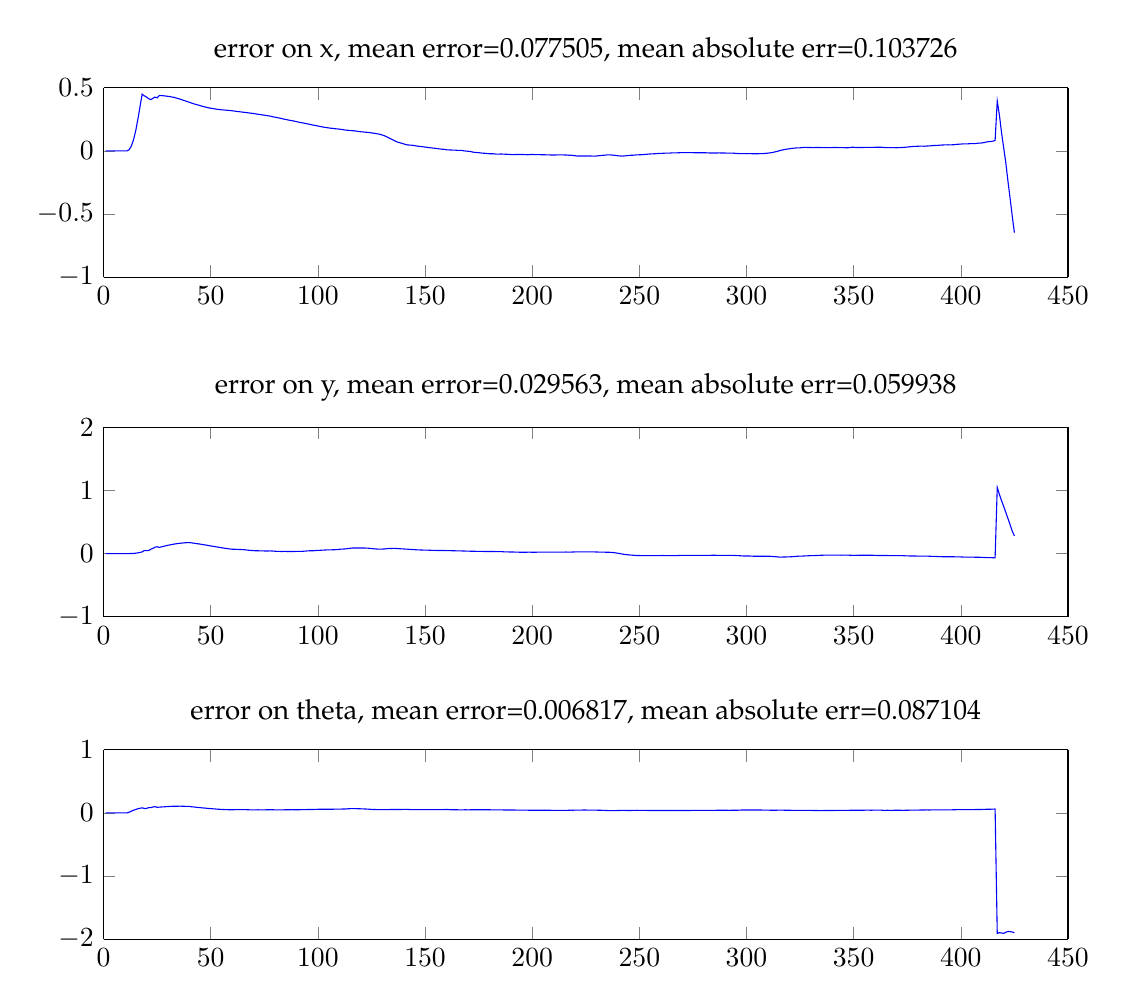
\begin{tikzpicture}

\begin{axis}[%
width=4.822in,
height=0.947in,
at={(0.809in,3.31in)},
scale only axis,
separate axis lines,
every outer x axis line/.append style={black},
every x tick label/.append style={font=\color{black}},
xmin=0,
xmax=450,
every outer y axis line/.append style={black},
every y tick label/.append style={font=\color{black}},
ymin=-1,
ymax=0.5,
axis background/.style={fill=white},
title={error on x, mean error=0.077505, mean absolute err=0.103726}
]
\addplot [color=blue,solid,forget plot]
  table[row sep=crcr]{%
1	0\\
2	0\\
3	0\\
4	0\\
5	0\\
6	0\\
7	0\\
8	0\\
9	0\\
10	0\\
11	0\\
12	0.00955562137445424\\
13	0.0392114902415333\\
14	0.0889396820844108\\
15	0.158714707843808\\
16	0.24851052301998\\
17	0.348779118151642\\
18	0.448990588271203\\
19	0.435665576371415\\
20	0.426386638613298\\
21	0.41323312084001\\
22	0.405570535111214\\
23	0.415423690052686\\
24	0.425647195648471\\
25	0.41932933819804\\
26	0.438241061077142\\
27	0.43744461096412\\
28	0.436068283573504\\
29	0.43402443557718\\
30	0.431880931625316\\
31	0.429308431132644\\
32	0.426047223843889\\
33	0.422942933492238\\
34	0.41822086950343\\
35	0.413041438924649\\
36	0.407777357263298\\
37	0.402068752332956\\
38	0.396309533531984\\
39	0.390649374068324\\
40	0.384449067761939\\
41	0.37873994330238\\
42	0.373016206261361\\
43	0.36794386060948\\
44	0.36339957234887\\
45	0.358401310461349\\
46	0.35325516005693\\
47	0.349158746312148\\
48	0.344720169096946\\
49	0.340602305418412\\
50	0.337413340397827\\
51	0.334970322352831\\
52	0.331897992738868\\
53	0.329111899031455\\
54	0.327362031617947\\
55	0.324873203182057\\
56	0.323642648305071\\
57	0.322213405771855\\
58	0.320839816435678\\
59	0.319061402179902\\
60	0.317436767422851\\
61	0.314817957479482\\
62	0.31250963634038\\
63	0.310899901811436\\
64	0.308434999957021\\
65	0.306326991429127\\
66	0.30427458685454\\
67	0.302438725757622\\
68	0.299652672568901\\
69	0.297531484201622\\
70	0.295503526752664\\
71	0.292805718093564\\
72	0.289812260300543\\
73	0.287838347214463\\
74	0.284734691873258\\
75	0.2828454994902\\
76	0.279469917582126\\
77	0.276875571943353\\
78	0.274484376370387\\
79	0.269559557525994\\
80	0.266677921117892\\
81	0.263399268379731\\
82	0.259858427743471\\
83	0.25582544409336\\
84	0.251656941053591\\
85	0.248932655761976\\
86	0.244534919692444\\
87	0.241671980482481\\
88	0.238599470930703\\
89	0.234916717328583\\
90	0.231462448258341\\
91	0.227376469323073\\
92	0.223788499248625\\
93	0.221106094145662\\
94	0.217429822028773\\
95	0.214307773499717\\
96	0.210712870473911\\
97	0.206791792008868\\
98	0.203242336575057\\
99	0.200485072195162\\
100	0.196627259505142\\
101	0.193215506657154\\
102	0.190033094212229\\
103	0.186781096564292\\
104	0.184134683904849\\
105	0.18173769139235\\
106	0.179165802437637\\
107	0.17795523693189\\
108	0.1752067935225\\
109	0.173778620733589\\
110	0.171811587427811\\
111	0.169561648900068\\
112	0.167017177819268\\
113	0.163915941100944\\
114	0.162981008032816\\
115	0.160665258741082\\
116	0.159652996395314\\
117	0.158666928981948\\
118	0.155733891950412\\
119	0.15347810794699\\
120	0.151144622976801\\
121	0.14976971192584\\
122	0.147829166197601\\
123	0.146796420258486\\
124	0.144691588367255\\
125	0.142258589290547\\
126	0.139557746539811\\
127	0.137135149707021\\
128	0.133772652634052\\
129	0.131138101346448\\
130	0.125457558896898\\
131	0.119587655429115\\
132	0.11235297153017\\
133	0.104131382732575\\
134	0.0956141164263293\\
135	0.0870297334066485\\
136	0.0780346225637452\\
137	0.0701850203243506\\
138	0.0656815081675575\\
139	0.0601817090147012\\
140	0.0551897380336186\\
141	0.0499609186480487\\
142	0.0462178140058942\\
143	0.0455648793092731\\
144	0.0443501091498142\\
145	0.0416809973991459\\
146	0.0387386309000295\\
147	0.0359771428693012\\
148	0.0345908081920854\\
149	0.0321802304786782\\
150	0.0299069067415996\\
151	0.0279479854900888\\
152	0.0250582771060248\\
153	0.0231441408591557\\
154	0.0215046209427907\\
155	0.0194971271929703\\
156	0.016932830617824\\
157	0.0146889943220643\\
158	0.0128237135859131\\
159	0.0117736808716007\\
160	0.00837920114845403\\
161	0.00706799072916198\\
162	0.0069353588993124\\
163	0.00532743590496665\\
164	0.0057594250889359\\
165	0.00405877584465308\\
166	0.00416213281380884\\
167	0.00351013125471944\\
168	0.000525160955719528\\
169	-0.00165606186867251\\
170	-0.00324659923894366\\
171	-0.00517570374900345\\
172	-0.00864719799412406\\
173	-0.0120322439917651\\
174	-0.0132236925551954\\
175	-0.01432906756955\\
176	-0.0169181494825867\\
177	-0.0186307656464759\\
178	-0.019422216188353\\
179	-0.0216640547734421\\
180	-0.0228826490842966\\
181	-0.0232517860229109\\
182	-0.0234235852471336\\
183	-0.0258270658325213\\
184	-0.0264196008799082\\
185	-0.0253711352868127\\
186	-0.0254914926409988\\
187	-0.0264131479232699\\
188	-0.0271633502294932\\
189	-0.0281228020222937\\
190	-0.0291696313398369\\
191	-0.0303556372796816\\
192	-0.0287622454736471\\
193	-0.0292756969203349\\
194	-0.0287866397241228\\
195	-0.0294682900039369\\
196	-0.0292876104351496\\
197	-0.0300173250626408\\
198	-0.0310645050088176\\
199	-0.0291380945707562\\
200	-0.0293775628418942\\
201	-0.0294817155495544\\
202	-0.0295716668199475\\
203	-0.0296736710690801\\
204	-0.0307080636856227\\
205	-0.0314337656899077\\
206	-0.0313337360418959\\
207	-0.0318514206246974\\
208	-0.0324055970135397\\
209	-0.0328141926166836\\
210	-0.0332734466693267\\
211	-0.0328754591400511\\
212	-0.0319168809599883\\
213	-0.0316654129143554\\
214	-0.0317648518025191\\
215	-0.0326529311653161\\
216	-0.033169197488494\\
217	-0.0347532512155926\\
218	-0.0343986909671461\\
219	-0.0367243224295528\\
220	-0.0388334929002294\\
221	-0.041170295084596\\
222	-0.04062463718566\\
223	-0.041115224414968\\
224	-0.0409489604567721\\
225	-0.0412345910567975\\
226	-0.040392955702778\\
227	-0.0408703924843987\\
228	-0.0415988640729736\\
229	-0.0417946308191937\\
230	-0.0410774471549367\\
231	-0.0389098482359582\\
232	-0.0374402471825377\\
233	-0.0352196579848361\\
234	-0.034196746472448\\
235	-0.0323262415602361\\
236	-0.0318870871831134\\
237	-0.0328811512102032\\
238	-0.0346808707828128\\
239	-0.0366819737475659\\
240	-0.0391416919251792\\
241	-0.0404606287102514\\
242	-0.0416604814690995\\
243	-0.0404871201409449\\
244	-0.0384633489327069\\
245	-0.0369856437573137\\
246	-0.0351435998906933\\
247	-0.0346840782029307\\
248	-0.0330037401435366\\
249	-0.0320048934744577\\
250	-0.0312921480410555\\
251	-0.0308511602684902\\
252	-0.0290753751125976\\
253	-0.0284458013294202\\
254	-0.0262996026713864\\
255	-0.0248749669030683\\
256	-0.0240666184553522\\
257	-0.0232357283393547\\
258	-0.0219463304429368\\
259	-0.0207585567018373\\
260	-0.0204039855851832\\
261	-0.0194512758012291\\
262	-0.0183402671464155\\
263	-0.0179621571494586\\
264	-0.0179874138230218\\
265	-0.0167223600056943\\
266	-0.016418063032722\\
267	-0.015808085835781\\
268	-0.0155566578901905\\
269	-0.0147974254932368\\
270	-0.0138118278949921\\
271	-0.0145767141577497\\
272	-0.0142179274780423\\
273	-0.0142239238510582\\
274	-0.0141834192793251\\
275	-0.0146284091755984\\
276	-0.0149879325247113\\
277	-0.0149279501896089\\
278	-0.0152285993117536\\
279	-0.0152079634080629\\
280	-0.0155761493495108\\
281	-0.0154415628439022\\
282	-0.0164686672846388\\
283	-0.0170027937065607\\
284	-0.0175654581058833\\
285	-0.0167975582649564\\
286	-0.0173242494812893\\
287	-0.0163426206633277\\
288	-0.0169887661932675\\
289	-0.0172893812603343\\
290	-0.0174626781962468\\
291	-0.0180615201552632\\
292	-0.0184662158693607\\
293	-0.018296260302578\\
294	-0.0187512428153074\\
295	-0.0200837689169608\\
296	-0.0213946858889997\\
297	-0.0217541441784901\\
298	-0.0221704639394957\\
299	-0.0223510161541256\\
300	-0.0227020554381259\\
301	-0.0222081556185758\\
302	-0.0224547691532484\\
303	-0.0230497211537015\\
304	-0.0225861249615651\\
305	-0.0235976689900097\\
306	-0.0217549403020998\\
307	-0.0219877862679301\\
308	-0.0214099041134865\\
309	-0.0196927566177223\\
310	-0.018312570747578\\
311	-0.0160277499250485\\
312	-0.013498995026739\\
313	-0.00940962913620957\\
314	-0.00552964858768679\\
315	-0.000995041331664837\\
316	0.00408181558323006\\
317	0.00770983868214437\\
318	0.0109443009771657\\
319	0.0137152397756588\\
320	0.0164461060954562\\
321	0.018796828382472\\
322	0.021016238794386\\
323	0.0225207610843454\\
324	0.0237743486923923\\
325	0.02375450377663\\
326	0.0259596624374798\\
327	0.0268180321253491\\
328	0.0271097889630436\\
329	0.0260787329115222\\
330	0.026230197756238\\
331	0.0253812305590482\\
332	0.0262040951457689\\
333	0.0265848497472887\\
334	0.0265584663243121\\
335	0.0256677850244089\\
336	0.0257846471066525\\
337	0.026095379675755\\
338	0.0254014601804666\\
339	0.0259687003238733\\
340	0.0259289059224934\\
341	0.0265223445714722\\
342	0.0262966353783289\\
343	0.0253486697589529\\
344	0.0258619523548478\\
345	0.0252137463945954\\
346	0.0248275205393882\\
347	0.0242568606400066\\
348	0.025267826321095\\
349	0.0280362155916851\\
350	0.0281384291801583\\
351	0.0263348408400796\\
352	0.0260494906504856\\
353	0.0268159103272261\\
354	0.0266245003036203\\
355	0.0269040364271818\\
356	0.0269926273987346\\
357	0.0273224638094702\\
358	0.0269093218178247\\
359	0.027058878922209\\
360	0.0279253754572868\\
361	0.028567712038428\\
362	0.0285587958909184\\
363	0.0282340058078625\\
364	0.0267119459906313\\
365	0.0255291642579323\\
366	0.0251527909283054\\
367	0.0248808104228313\\
368	0.0254515384050025\\
369	0.0251261627986612\\
370	0.0244410855892081\\
371	0.0255690155159203\\
372	0.0258420062292641\\
373	0.0270679473257025\\
374	0.0282523464108302\\
375	0.0298611413532006\\
376	0.0318105490805229\\
377	0.0336451308452839\\
378	0.0351342755915183\\
379	0.0356579562460544\\
380	0.0361514364242843\\
381	0.037539267275762\\
382	0.0373145398268397\\
383	0.0364879985938658\\
384	0.0379103565988466\\
385	0.038892874597489\\
386	0.0400525041069084\\
387	0.0421124243494271\\
388	0.0419533092149051\\
389	0.0430977739509606\\
390	0.0444403500048289\\
391	0.0459472750486776\\
392	0.046596584617095\\
393	0.0469973950933333\\
394	0.0479283628134117\\
395	0.0471331505200681\\
396	0.0478312131583585\\
397	0.0489324130993042\\
398	0.0513978012995161\\
399	0.0523256685480814\\
400	0.0533751619377998\\
401	0.0551549118504223\\
402	0.0548826866723819\\
403	0.0551350082863854\\
404	0.0564354404307549\\
405	0.0571772716441481\\
406	0.0566950824105825\\
407	0.0577404406298712\\
408	0.0603861019091073\\
409	0.0608685420673536\\
410	0.0633270185817429\\
411	0.0657088066599767\\
412	0.070246361667913\\
413	0.0724386402763236\\
414	0.0739271321927358\\
415	0.07708445932222\\
416	0.0818613044672585\\
417	0.394268464142862\\
418	0.284029860482681\\
419	0.145429173534072\\
420	0.0235621123749868\\
421	-0.095795500303318\\
422	-0.241390595480607\\
423	-0.376031097452248\\
424	-0.51675763777199\\
425	-0.648438665990288\\
};
\end{axis}

\begin{axis}[%
width=4.822in,
height=0.947in,
at={(0.809in,1.612in)},
scale only axis,
separate axis lines,
every outer x axis line/.append style={black},
every x tick label/.append style={font=\color{black}},
xmin=0,
xmax=450,
every outer y axis line/.append style={black},
every y tick label/.append style={font=\color{black}},
ymin=-1,
ymax=2,
axis background/.style={fill=white},
title={error on y, mean error=0.029563, mean absolute err=0.059938}
]
\addplot [color=blue,solid,forget plot]
  table[row sep=crcr]{%
1	0\\
2	0\\
3	0\\
4	0\\
5	0\\
6	0\\
7	0\\
8	0\\
9	0\\
10	0\\
11	0\\
12	4.68923517553624e-05\\
13	0.000622000891454959\\
14	0.00236112381575805\\
15	0.00572348872527853\\
16	0.011053629849223\\
17	0.0179379357724753\\
18	0.0255909506065986\\
19	0.047605535859966\\
20	0.0467104321984274\\
21	0.0472152638513229\\
22	0.0683883760158667\\
23	0.0812000474322988\\
24	0.100394010444185\\
25	0.108169250275792\\
26	0.0973352124346576\\
27	0.106257382851095\\
28	0.114991934625321\\
29	0.12328624469211\\
30	0.130819213630006\\
31	0.137687086730886\\
32	0.144422444790804\\
33	0.150711512986103\\
34	0.156012266594144\\
35	0.16087923748531\\
36	0.16454921595292\\
37	0.167948301385888\\
38	0.170895976051161\\
39	0.172918759698165\\
40	0.17419343104948\\
41	0.169652586966969\\
42	0.164871518951504\\
43	0.159574826586946\\
44	0.154999946017788\\
45	0.150217802835201\\
46	0.144785765537998\\
47	0.138716651675221\\
48	0.133495819024522\\
49	0.127222092372599\\
50	0.121601422808288\\
51	0.115416023784177\\
52	0.109726349200436\\
53	0.104315526643053\\
54	0.0979059190513153\\
55	0.092029721431741\\
56	0.0871930909761884\\
57	0.0819943957048241\\
58	0.0771527848467358\\
59	0.0728143562151071\\
60	0.0688845034983552\\
61	0.0679820845046016\\
62	0.0671289969900016\\
63	0.0658217373032199\\
64	0.0640787552329312\\
65	0.0623865223826178\\
66	0.0599910060968039\\
67	0.0557199083034791\\
68	0.0517392832004305\\
69	0.0489512397569173\\
70	0.04643476829575\\
71	0.044685676861245\\
72	0.0443015384759087\\
73	0.0432452145152001\\
74	0.0427372861732911\\
75	0.0414440746148573\\
76	0.0408126030708178\\
77	0.0411721963662172\\
78	0.042074157578616\\
79	0.0398710426389868\\
80	0.0367909705012293\\
81	0.0350159908051499\\
82	0.0338354527369541\\
83	0.0333550867409075\\
84	0.0336782954111664\\
85	0.0336655084949271\\
86	0.0332093108705825\\
87	0.0331018962612869\\
88	0.0330123770826286\\
89	0.0331758490484432\\
90	0.0340050612770113\\
91	0.0341511607677354\\
92	0.0347851358392148\\
93	0.0358869085517795\\
94	0.0385976697243985\\
95	0.0418620077490258\\
96	0.0439003075051783\\
97	0.0442667086475685\\
98	0.0452414027985625\\
99	0.0481889192587985\\
100	0.0506679793093143\\
101	0.0517131877660409\\
102	0.0537697052389117\\
103	0.0559205053666907\\
104	0.0576250647298995\\
105	0.0583596022354709\\
106	0.0586326584850104\\
107	0.060271646890095\\
108	0.0612246177181028\\
109	0.0634217648849238\\
110	0.0674124547243282\\
111	0.0702500666171558\\
112	0.0718860507029477\\
113	0.074142479886158\\
114	0.0787204363905951\\
115	0.0831311773863971\\
116	0.0881111280536199\\
117	0.0878724581467051\\
118	0.0888427042572986\\
119	0.0879844391635958\\
120	0.0880244481072061\\
121	0.087665814379234\\
122	0.0875057838330932\\
123	0.0865439017790072\\
124	0.0832034921404589\\
125	0.0790671789287561\\
126	0.0763275526599085\\
127	0.0730377344021792\\
128	0.0709721725900549\\
129	0.0705876235040698\\
130	0.0710489766627719\\
131	0.0728531978108369\\
132	0.076890906492501\\
133	0.0795885751012038\\
134	0.0810941251839004\\
135	0.0811383236162118\\
136	0.0812811044382218\\
137	0.0799009136276903\\
138	0.0772259291578441\\
139	0.0749308710210517\\
140	0.0730787478747437\\
141	0.0708702775428387\\
142	0.0688310812920245\\
143	0.0659185408389251\\
144	0.0643278686975428\\
145	0.0624850284848057\\
146	0.0596811284285672\\
147	0.0588180993282954\\
148	0.0565460996310438\\
149	0.0556663248066478\\
150	0.0551128194852324\\
151	0.0541402001855795\\
152	0.0530474353655208\\
153	0.0514578851728134\\
154	0.0511478356325434\\
155	0.0497719766787994\\
156	0.0487195957870887\\
157	0.0490341468880007\\
158	0.0485475969874996\\
159	0.0479274094172202\\
160	0.0472202900592786\\
161	0.046875570204036\\
162	0.0461427284494249\\
163	0.0439156620092938\\
164	0.0438762346671897\\
165	0.0433461716965899\\
166	0.0425701112181622\\
167	0.0417091626195569\\
168	0.040498671934893\\
169	0.0394240991806996\\
170	0.0389011639631827\\
171	0.0374628614805257\\
172	0.0370480645980251\\
173	0.03617528487489\\
174	0.0356006009559549\\
175	0.0352857390105976\\
176	0.0349742832868882\\
177	0.0338104626417151\\
178	0.0329185618385566\\
179	0.0335442701254083\\
180	0.0329014987494451\\
181	0.0332651450105246\\
182	0.032112813971465\\
183	0.0316581065643433\\
184	0.0305214880457942\\
185	0.0300209581992101\\
186	0.0299631173135966\\
187	0.0271647549573943\\
188	0.0265139877044032\\
189	0.0258152880772746\\
190	0.0250875666946637\\
191	0.0245169921965873\\
192	0.0236463609863948\\
193	0.0221523463373616\\
194	0.0216641482931781\\
195	0.0215535999480885\\
196	0.0211114283809755\\
197	0.0208840301433346\\
198	0.022029480348813\\
199	0.0219567071104176\\
200	0.0210915996412284\\
201	0.0211019159115988\\
202	0.0216510587331573\\
203	0.0222461441120618\\
204	0.02215852492035\\
205	0.022775667602426\\
206	0.0223152772615407\\
207	0.0226776268387496\\
208	0.0220454105284773\\
209	0.022183164848828\\
210	0.0225329563272396\\
211	0.0219311344501474\\
212	0.0217503745867251\\
213	0.0229485517627523\\
214	0.0230782042165405\\
215	0.0238784138189185\\
216	0.0240952499911433\\
217	0.023186364831373\\
218	0.0233312657117963\\
219	0.0250307010626223\\
220	0.0260749676944343\\
221	0.0270257637114142\\
222	0.0266148502952337\\
223	0.0259814843241202\\
224	0.0258482913320162\\
225	0.0258261111268894\\
226	0.0264608922006317\\
227	0.0267446723288547\\
228	0.0258908783665177\\
229	0.0261323121983335\\
230	0.0250827080926079\\
231	0.0237096638989023\\
232	0.022974021612022\\
233	0.0218724922027196\\
234	0.0217640248008504\\
235	0.0211661924295186\\
236	0.0203059128011827\\
237	0.0178063859324631\\
238	0.0154438358474387\\
239	0.0104115658249846\\
240	0.00521267878915843\\
241	-0.00132398522214494\\
242	-0.00720852787965143\\
243	-0.013129185285397\\
244	-0.0173700286563623\\
245	-0.0204176349057725\\
246	-0.0241229703974017\\
247	-0.0259460522162556\\
248	-0.0291270682168943\\
249	-0.0314763305705412\\
250	-0.0310136463197868\\
251	-0.0323423834979373\\
252	-0.0317913715573361\\
253	-0.0317595596216496\\
254	-0.0319421210096476\\
255	-0.032503137821795\\
256	-0.0327471935264505\\
257	-0.0326566537956481\\
258	-0.0322659889962154\\
259	-0.0322991745588013\\
260	-0.0315757334632831\\
261	-0.0312502222340481\\
262	-0.0318634017667758\\
263	-0.0315120996609757\\
264	-0.0314593334944799\\
265	-0.0316837878831677\\
266	-0.0330393539699187\\
267	-0.0324329478119587\\
268	-0.0311785119557815\\
269	-0.0293492290290267\\
270	-0.0293326198860875\\
271	-0.0278408377342743\\
272	-0.0279788747748011\\
273	-0.0279811675403145\\
274	-0.0281211195452098\\
275	-0.0281145744958948\\
276	-0.02932872020118\\
277	-0.0286629475707656\\
278	-0.0275089727079099\\
279	-0.0284600412894118\\
280	-0.0289729707673594\\
281	-0.0280955495701338\\
282	-0.0279447866912754\\
283	-0.0278728238920891\\
284	-0.0271985801359556\\
285	-0.0267644329184265\\
286	-0.0277569926933516\\
287	-0.0278675215804451\\
288	-0.0278402484473474\\
289	-0.0291555808619339\\
290	-0.0281530360021485\\
291	-0.0279375240867079\\
292	-0.02759652323914\\
293	-0.0275735913302011\\
294	-0.0292257758804713\\
295	-0.0309150498239656\\
296	-0.0325540651024028\\
297	-0.0346112482203491\\
298	-0.0369986183034605\\
299	-0.0393179217772612\\
300	-0.0391855066972955\\
301	-0.0382072218021143\\
302	-0.0399711601715449\\
303	-0.041506825115448\\
304	-0.042423559445055\\
305	-0.0426435175189006\\
306	-0.0425362669470744\\
307	-0.0429309060542487\\
308	-0.0426742641891238\\
309	-0.0426387177398162\\
310	-0.0414913162283934\\
311	-0.0432931992569312\\
312	-0.0455932621799668\\
313	-0.0482277784033442\\
314	-0.0512354259294128\\
315	-0.0547409330052453\\
316	-0.056504078972182\\
317	-0.0547512037576237\\
318	-0.0544627422437358\\
319	-0.0531713741727398\\
320	-0.0518892527341741\\
321	-0.050232837394681\\
322	-0.0481881639564499\\
323	-0.0447496876434794\\
324	-0.0418865713774998\\
325	-0.0408115996800866\\
326	-0.0398142486774979\\
327	-0.0381580547735982\\
328	-0.0364362599739536\\
329	-0.0343951928571808\\
330	-0.0328621497642096\\
331	-0.0324144662366646\\
332	-0.0311511964195628\\
333	-0.0300549843880269\\
334	-0.0285002797697622\\
335	-0.0266323263339654\\
336	-0.0255659174845135\\
337	-0.0247495741020138\\
338	-0.0250320711610907\\
339	-0.0250534540600267\\
340	-0.0252802936398933\\
341	-0.0255715479310687\\
342	-0.0250117943784609\\
343	-0.0242614690108915\\
344	-0.0258184179677006\\
345	-0.0256939336381192\\
346	-0.0252150208713262\\
347	-0.0251248813335927\\
348	-0.0258856117946777\\
349	-0.0276992891248087\\
350	-0.0281163189077125\\
351	-0.0273971544241745\\
352	-0.0276301615300003\\
353	-0.0272207270784222\\
354	-0.0265068959629344\\
355	-0.0269374075652937\\
356	-0.0272225780000284\\
357	-0.0265620913756681\\
358	-0.0272243205635014\\
359	-0.0272723420276719\\
360	-0.0290009621885039\\
361	-0.0299404043024802\\
362	-0.0304430380491771\\
363	-0.0307125606720584\\
364	-0.0306194689299994\\
365	-0.0308709036776502\\
366	-0.0313537168880726\\
367	-0.0324337734932962\\
368	-0.0332363402262583\\
369	-0.0329058154984176\\
370	-0.0334593555802982\\
371	-0.0327332114651702\\
372	-0.0327640783127192\\
373	-0.0332279043972772\\
374	-0.0354354040230893\\
375	-0.0371915852697704\\
376	-0.0377701762463039\\
377	-0.0383589040339931\\
378	-0.0382964122389877\\
379	-0.0388261474452305\\
380	-0.0404833558710926\\
381	-0.040640611800776\\
382	-0.0399551814019947\\
383	-0.0395453702411386\\
384	-0.0404445663412476\\
385	-0.0415713830137339\\
386	-0.0432041372776264\\
387	-0.0451868056801179\\
388	-0.0450010045123492\\
389	-0.0469529219654214\\
390	-0.0488588025959293\\
391	-0.0493129705974624\\
392	-0.0503357644024183\\
393	-0.0503855657771553\\
394	-0.0500398756234182\\
395	-0.049834114314137\\
396	-0.0509652763569051\\
397	-0.0508979690511824\\
398	-0.0533356299923988\\
399	-0.0527698874271039\\
400	-0.0535101626282217\\
401	-0.0552783645768393\\
402	-0.0552360270076799\\
403	-0.0552578444192693\\
404	-0.0574757505090333\\
405	-0.0568120408125607\\
406	-0.0570882417264662\\
407	-0.0581533120973257\\
408	-0.059064974816692\\
409	-0.0588463661568883\\
410	-0.060716053701108\\
411	-0.0620082273078446\\
412	-0.0640457354666766\\
413	-0.0641392595454715\\
414	-0.0650144454845298\\
415	-0.065747137106335\\
416	-0.0681368081206442\\
417	1.04577322851601\\
418	0.938562739659491\\
419	0.838659318763967\\
420	0.746595332053542\\
421	0.651385995591586\\
422	0.555002553560153\\
423	0.457169682709059\\
424	0.357092579072047\\
425	0.279719070485088\\
};
\end{axis}

\begin{axis}[%
width=4.822in,
height=0.947in,
at={(0.809in,0in)},
scale only axis,
separate axis lines,
every outer x axis line/.append style={black},
every x tick label/.append style={font=\color{black}},
xmin=0,
xmax=450,
every outer y axis line/.append style={black},
every y tick label/.append style={font=\color{black}},
ymin=-2,
ymax=1,
axis background/.style={fill=white},
title={error on theta, mean error=0.006817, mean absolute err=0.087104}
]
\addplot [color=blue,solid,forget plot]
  table[row sep=crcr]{%
1	0\\
2	0\\
3	0\\
4	0\\
5	0\\
6	0\\
7	0\\
8	0\\
9	0\\
10	0\\
11	0\\
12	0.00977531043779623\\
13	0.0270356169185559\\
14	0.0416765421666323\\
15	0.0538955052568495\\
16	0.0642116793144671\\
17	0.0727510351741865\\
18	0.0795825528899776\\
19	0.0689656154764076\\
20	0.0696539257530713\\
21	0.0811469332254551\\
22	0.0824757871733963\\
23	0.0915601712151446\\
24	0.0987179137086245\\
25	0.0869050120081116\\
26	0.0902760032884387\\
27	0.0927883237344869\\
28	0.0946004817728974\\
29	0.0973460190464359\\
30	0.100035359283406\\
31	0.101332620886968\\
32	0.103647926365973\\
33	0.10458073625241\\
34	0.105051329392673\\
35	0.105099720263969\\
36	0.105400950425366\\
37	0.104264039771459\\
38	0.103362052661142\\
39	0.102541162598473\\
40	0.101503217846374\\
41	0.096594875152678\\
42	0.093334563261056\\
43	0.0890833048872581\\
44	0.0856539510332204\\
45	0.0827443430565808\\
46	0.0787998618409014\\
47	0.076128555914313\\
48	0.0731563396899286\\
49	0.0687868436190509\\
50	0.0666530374408274\\
51	0.064175212054562\\
52	0.0617746013534846\\
53	0.0580140494081371\\
54	0.0565277114452827\\
55	0.0542648178614247\\
56	0.0522694336471088\\
57	0.0506656779676691\\
58	0.0497926060880411\\
59	0.0492801697206193\\
60	0.048600712928883\\
61	0.0498277098592879\\
62	0.0498806104663139\\
63	0.0500936258260887\\
64	0.0505060096110936\\
65	0.0507593918824338\\
66	0.0506815471210809\\
67	0.0495491854136767\\
68	0.0477802079293608\\
69	0.0468290635420257\\
70	0.0467383417665843\\
71	0.0475080257916405\\
72	0.0481804952112621\\
73	0.0472038145095404\\
74	0.0472675686950925\\
75	0.0478040350257167\\
76	0.0480502768590689\\
77	0.0482697173198017\\
78	0.0498948404458921\\
79	0.0487558903775578\\
80	0.0472624526750627\\
81	0.0459330529485178\\
82	0.0466172489423196\\
83	0.0474162605671489\\
84	0.0479020505575907\\
85	0.0482540849318482\\
86	0.048699848491311\\
87	0.0491678945426535\\
88	0.0498756316223985\\
89	0.049461369218021\\
90	0.0490980012913429\\
91	0.0490590851517063\\
92	0.0498254241070688\\
93	0.0504212434140543\\
94	0.0512219286934723\\
95	0.0520501648569183\\
96	0.0527081302293415\\
97	0.0529757521964216\\
98	0.0532486020845475\\
99	0.0549865758539219\\
100	0.0559538902623373\\
101	0.0564227416615113\\
102	0.057380847814041\\
103	0.0574754870768026\\
104	0.0573389125847439\\
105	0.056980037819077\\
106	0.0567143994198163\\
107	0.0572301392692136\\
108	0.0580509211327334\\
109	0.0579991423147677\\
110	0.0590359151019619\\
111	0.0596167869760893\\
112	0.060611924584951\\
113	0.0609559942141202\\
114	0.0639882227655297\\
115	0.0656869920244851\\
116	0.0663644908412717\\
117	0.0658833165133519\\
118	0.066050137533562\\
119	0.0648290638697531\\
120	0.0637546670784381\\
121	0.0619532630703472\\
122	0.0611641843811563\\
123	0.0593125943241386\\
124	0.0569232392415229\\
125	0.0550074549863546\\
126	0.053550464954772\\
127	0.0523000242601355\\
128	0.0509273778954467\\
129	0.0506687076515067\\
130	0.0506647071202924\\
131	0.0506320718355933\\
132	0.0509066963380036\\
133	0.0517453117800075\\
134	0.052199021635758\\
135	0.0526200002638668\\
136	0.0537678026152917\\
137	0.0529413568774468\\
138	0.0535807931585177\\
139	0.0532730433663127\\
140	0.0541691841209824\\
141	0.0542493936368196\\
142	0.053699303830145\\
143	0.0518596552227866\\
144	0.0509100803693667\\
145	0.0518486588749258\\
146	0.0513125776173124\\
147	0.051081030341745\\
148	0.0509752103660714\\
149	0.051011090800746\\
150	0.0506675294506351\\
151	0.0517917224376943\\
152	0.0512304435796178\\
153	0.0498214111034825\\
154	0.0504496775721606\\
155	0.0502244974026462\\
156	0.0512102992517178\\
157	0.0516121751237288\\
158	0.0512408162388533\\
159	0.0523723393782953\\
160	0.0523439493617808\\
161	0.0519167657620314\\
162	0.0492600303977513\\
163	0.0498540617047718\\
164	0.0486630497897194\\
165	0.0482890940532883\\
166	0.047507209134511\\
167	0.0467813210029169\\
168	0.0475407994069146\\
169	0.0487111070379207\\
170	0.0469659939285285\\
171	0.0480405542900741\\
172	0.0493222727871094\\
173	0.049686558941139\\
174	0.0490877988592962\\
175	0.0486098447637078\\
176	0.0494745879591476\\
177	0.0491290768982635\\
178	0.0489386243612957\\
179	0.0497327533678749\\
180	0.049186906934505\\
181	0.0470064071638543\\
182	0.0468154928280571\\
183	0.0467285699734914\\
184	0.0461666043624409\\
185	0.045740706393727\\
186	0.046184526417635\\
187	0.0452612000193584\\
188	0.0451151030275465\\
189	0.0450560099922952\\
190	0.0451107970764091\\
191	0.045684310284992\\
192	0.0442275128312755\\
193	0.0431649035204504\\
194	0.0435650711935764\\
195	0.0426459434161814\\
196	0.0423425721218669\\
197	0.0425447610858867\\
198	0.041899232880934\\
199	0.0409232384112483\\
200	0.0412305792121508\\
201	0.0403959089426915\\
202	0.0408347382398575\\
203	0.0410981101614878\\
204	0.0406699877794128\\
205	0.0413888526738644\\
206	0.0413804279082779\\
207	0.0409449688844985\\
208	0.0407091190860784\\
209	0.0398849660781178\\
210	0.0400151339533745\\
211	0.0395282264144212\\
212	0.0389462801958027\\
213	0.0387635943996862\\
214	0.0395228068420832\\
215	0.0397225117091615\\
216	0.0399153471840248\\
217	0.0401161751006538\\
218	0.0418603338643173\\
219	0.0415989703043818\\
220	0.0419912242293132\\
221	0.0438984591820404\\
222	0.043176770070156\\
223	0.0439384804919465\\
224	0.0441726157093436\\
225	0.0446507918469452\\
226	0.0426522030416892\\
227	0.0434076941104284\\
228	0.0433795126615752\\
229	0.0436992215573682\\
230	0.042214476097751\\
231	0.0406900418129057\\
232	0.0408253327263646\\
233	0.0387568329752543\\
234	0.0379867125202589\\
235	0.0364454094926194\\
236	0.0341369414600949\\
237	0.0346421790683791\\
238	0.0352686773600537\\
239	0.0354242003981011\\
240	0.0374010831816713\\
241	0.0375395655060125\\
242	0.0384481909079741\\
243	0.0386789510053616\\
244	0.0372105567130578\\
245	0.0370772790983138\\
246	0.0371173077415232\\
247	0.038632389808348\\
248	0.0399145058368298\\
249	0.0401041280497765\\
250	0.0396172329226561\\
251	0.0387709214241436\\
252	0.0388969057191808\\
253	0.0384949288721428\\
254	0.0368599194676165\\
255	0.0374176664011632\\
256	0.0371990126927884\\
257	0.037646484341554\\
258	0.0373807136005109\\
259	0.0368696144681735\\
260	0.0370361627237106\\
261	0.0376139631491057\\
262	0.0372174514975967\\
263	0.0369004323943205\\
264	0.0374263418812593\\
265	0.036350891217082\\
266	0.0380692786284671\\
267	0.03709766545715\\
268	0.0371457871096181\\
269	0.03685896190553\\
270	0.0374783330584982\\
271	0.0374976013854482\\
272	0.0369971734265935\\
273	0.0377677035930013\\
274	0.0377515919248168\\
275	0.0386534401291083\\
276	0.0389515402594878\\
277	0.039138197212055\\
278	0.0393057646726902\\
279	0.0395234233450807\\
280	0.0395889824271656\\
281	0.0386825988706647\\
282	0.038319906839007\\
283	0.0385276397797121\\
284	0.0382986212563381\\
285	0.0389139641848164\\
286	0.0401692318604532\\
287	0.0402535543841109\\
288	0.0404105100060157\\
289	0.0404013168122095\\
290	0.0404787471918038\\
291	0.0402860794755497\\
292	0.0397273764120083\\
293	0.0405341512933433\\
294	0.040712464145189\\
295	0.0407220744543668\\
296	0.0414180002407836\\
297	0.0439466698184763\\
298	0.0441908483132849\\
299	0.0455775349973457\\
300	0.0443322353082714\\
301	0.0441025226257246\\
302	0.044427939609629\\
303	0.045141691093928\\
304	0.0454176539128603\\
305	0.0447030280368876\\
306	0.0444534806827761\\
307	0.0441710279225518\\
308	0.0429474991672851\\
309	0.0430922487255838\\
310	0.0428842971761512\\
311	0.0416140321145519\\
312	0.0415153048090566\\
313	0.0411991777917589\\
314	0.0412549738419967\\
315	0.0433429059930628\\
316	0.0420205147398294\\
317	0.042395473953146\\
318	0.04089277973649\\
319	0.040950180370622\\
320	0.0405160864978669\\
321	0.0398860171741164\\
322	0.0395367788877241\\
323	0.039326239408755\\
324	0.0384280949189053\\
325	0.0377890779186343\\
326	0.0391688465322098\\
327	0.0389689186674858\\
328	0.0377097841217262\\
329	0.0384226645556129\\
330	0.0379082430283688\\
331	0.0376935442541466\\
332	0.0375030253034421\\
333	0.036817599839555\\
334	0.035732017934599\\
335	0.0352577654834336\\
336	0.036606789955278\\
337	0.0372809166154688\\
338	0.0364083000611419\\
339	0.0376305567850395\\
340	0.0368448339410268\\
341	0.0367792455626308\\
342	0.0384295334133853\\
343	0.0377147796826547\\
344	0.0380739728984381\\
345	0.0387372415083629\\
346	0.0381295804115371\\
347	0.03877369260357\\
348	0.0398243276760999\\
349	0.0413570729078812\\
350	0.0407538411088977\\
351	0.0411404973806331\\
352	0.0409903941872241\\
353	0.0417062433069644\\
354	0.041645311761024\\
355	0.0417179540616726\\
356	0.0425349443454239\\
357	0.0424555474360249\\
358	0.0413227294401448\\
359	0.0419259525768094\\
360	0.0423095520078665\\
361	0.0422499234700009\\
362	0.0427234121684608\\
363	0.0418279470592759\\
364	0.039623447063013\\
365	0.0400373927252566\\
366	0.0401565465119376\\
367	0.0396206097294129\\
368	0.0394920059023063\\
369	0.0403591103615071\\
370	0.0403120728446353\\
371	0.0400694005597488\\
372	0.0401727025553749\\
373	0.0393824982805109\\
374	0.0401370089574593\\
375	0.040739372386505\\
376	0.0421515995390367\\
377	0.0437081145657467\\
378	0.0433091323796955\\
379	0.0428142601425296\\
380	0.0434232363263956\\
381	0.0443461145628268\\
382	0.0444581420556194\\
383	0.0451973489974886\\
384	0.046017681607978\\
385	0.0454430529706924\\
386	0.0457788648780353\\
387	0.0466322710131166\\
388	0.0468896338727438\\
389	0.0475482122673014\\
390	0.0474810700387378\\
391	0.0475812067604942\\
392	0.0476512862545553\\
393	0.0480227627986594\\
394	0.0474956731029161\\
395	0.0471282017218879\\
396	0.0479640646789079\\
397	0.0489697722375917\\
398	0.05001988939238\\
399	0.0507119545899268\\
400	0.0509392129780277\\
401	0.0501061224884989\\
402	0.0502456548234331\\
403	0.0509886733680744\\
404	0.0514464164756498\\
405	0.0513671481089659\\
406	0.0516014402831146\\
407	0.0520928477976454\\
408	0.0528645825674783\\
409	0.0532069514990292\\
410	0.0539637749653323\\
411	0.0541808790430691\\
412	0.0568576646283532\\
413	0.0572192722190525\\
414	0.0575362811964411\\
415	0.05827452235068\\
416	0.060250728183183\\
417	-1.91051987719597\\
418	-1.89776828530092\\
419	-1.90381691409292\\
420	-1.9079989677713\\
421	-1.89163238848583\\
422	-1.8791012385805\\
423	-1.88269743839444\\
424	-1.88652180485805\\
425	-1.90080860522801\\
};
\end{axis}
\end{tikzpicture}%}
	\caption{Mean pose error when the number of particles $M=1000$ (left) and $M=10000$ (right).}
	\label{fig:Tracking_Error_Map_2_M_1000_10000}
\end{figure}

\begin{figure}
	\centering
	\scalebox{0.5}{% This file was created by matlab2tikz.
%
%The latest updates can be retrieved from
%  http://www.mathworks.com/matlabcentral/fileexchange/22022-matlab2tikz-matlab2tikz
%where you can also make suggestions and rate matlab2tikz.
%
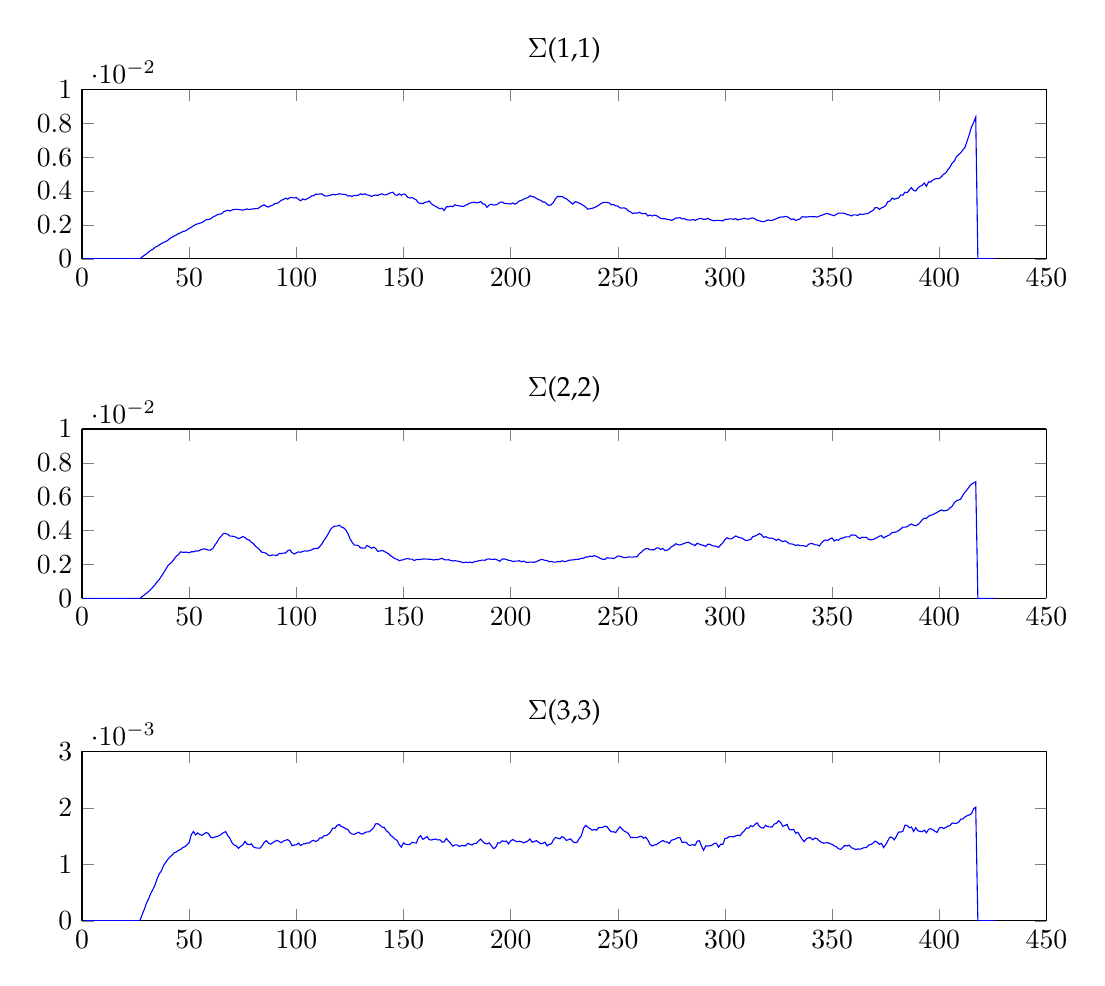
\begin{tikzpicture}

\begin{axis}[%
width=4.822in,
height=0.847in,
at={(0.809in,3.31in)},
scale only axis,
separate axis lines,
every outer x axis line/.append style={black},
every x tick label/.append style={font=\color{black}},
xmin=0,
xmax=450,
every outer y axis line/.append style={black},
every y tick label/.append style={font=\color{black}},
ymin=0,
ymax=0.01,
axis background/.style={fill=white},
title={$\Sigma\text{(1,1)}$}
]
\addplot [color=blue,solid,forget plot]
  table[row sep=crcr]{%
1	0\\
2	6.7964518221717e-33\\
3	4.12380832999582e-33\\
4	1.79338972048671e-31\\
5	2.09943714658428e-31\\
6	4.19429563088837e-32\\
7	1.92785780218943e-34\\
8	2.71105003432888e-33\\
9	5.44092680500726e-33\\
10	7.53069453980244e-33\\
11	3.07282460002099e-32\\
12	1.03095208249895e-33\\
13	8.14519921425032e-33\\
14	2.12546322691384e-32\\
15	4.81964450547356e-33\\
16	8.99461336189498e-30\\
17	6.10822466045698e-30\\
18	3.14657239042149e-29\\
19	3.40074116306215e-29\\
20	6.94028808788193e-29\\
21	7.89650555776789e-31\\
22	6.04576206766604e-29\\
23	6.04576206766604e-31\\
24	2.17647434435977e-29\\
25	9.77315945673116e-29\\
26	8.70589737743909e-29\\
27	1.71798349041188e-28\\
28	0.000104207825842498\\
29	0.000199063984388529\\
30	0.000289011252195975\\
31	0.000386609421233009\\
32	0.000497723931360076\\
33	0.00055238632959312\\
34	0.000671293705287079\\
35	0.00073321636338031\\
36	0.000808092886307675\\
37	0.000894203213566873\\
38	0.00096479094835832\\
39	0.00101961573346739\\
40	0.00108551801784442\\
41	0.0012029315692968\\
42	0.00127112610423876\\
43	0.00135194130334319\\
44	0.00140420219280578\\
45	0.00149029903020733\\
46	0.0015293457802968\\
47	0.00161005345380057\\
48	0.00163504108743009\\
49	0.00170269429029526\\
50	0.00179969681696039\\
51	0.00186408179497934\\
52	0.00194553677708479\\
53	0.00202448267584599\\
54	0.0020643324411251\\
55	0.00210118012233368\\
56	0.00214219776976477\\
57	0.00222535017140327\\
58	0.00231296651645396\\
59	0.00232002189089167\\
60	0.0023585593149447\\
61	0.00246041543822198\\
62	0.00251757609101002\\
63	0.00259247025600686\\
64	0.00263098943942239\\
65	0.00265183840402957\\
66	0.00277009096514636\\
67	0.00282805914092036\\
68	0.00286893895161976\\
69	0.0028211257400814\\
70	0.00287675858402678\\
71	0.00291976882810627\\
72	0.00292039917276943\\
73	0.00291571720979064\\
74	0.00289045225100451\\
75	0.00287580595481869\\
76	0.0028999060709163\\
77	0.00294626998379109\\
78	0.00290436037417054\\
79	0.0029349286522022\\
80	0.0029442984748768\\
81	0.0029646445648741\\
82	0.00296384190327248\\
83	0.00305187631899331\\
84	0.00313225655379945\\
85	0.00318810283433407\\
86	0.00308908305126551\\
87	0.00305566576806505\\
88	0.0031282311954691\\
89	0.00316275936787975\\
90	0.00326642940702168\\
91	0.00326976691476274\\
92	0.0033485960516417\\
93	0.00345274325997895\\
94	0.00349664816460482\\
95	0.00357900566185954\\
96	0.00352018473598365\\
97	0.00362059892745294\\
98	0.0036153826688336\\
99	0.00358991310159041\\
100	0.00361442518958742\\
101	0.00351220357441759\\
102	0.00342188272622207\\
103	0.00353572401939871\\
104	0.00348175461833107\\
105	0.00354115817101048\\
106	0.00360138195627168\\
107	0.003705972800184\\
108	0.00372157361648434\\
109	0.00381034068269952\\
110	0.00381284389185889\\
111	0.00382244094805622\\
112	0.0038233924177166\\
113	0.003725183773053\\
114	0.00370090017149712\\
115	0.00372623083587394\\
116	0.00375700363852797\\
117	0.00380506365098124\\
118	0.00377655508251521\\
119	0.00379417105561017\\
120	0.00384102829015692\\
121	0.00381596072503953\\
122	0.00380276239493871\\
123	0.00380183936761183\\
124	0.00370445935849201\\
125	0.0037249854674698\\
126	0.0036788610223889\\
127	0.00374619321630873\\
128	0.00373289575477972\\
129	0.00375927402040228\\
130	0.00383337898984563\\
131	0.00378333537682981\\
132	0.0038370302664505\\
133	0.00375977364947801\\
134	0.0037513170661044\\
135	0.00367484221719393\\
136	0.0037420332851256\\
137	0.00376362866002086\\
138	0.00373901807963076\\
139	0.00380544720553398\\
140	0.00383324063689533\\
141	0.00377682987744693\\
142	0.0037765251522282\\
143	0.00384767847156449\\
144	0.00389600287215423\\
145	0.00393254238991239\\
146	0.0037834907606723\\
147	0.00374525239230932\\
148	0.00383519226126649\\
149	0.00375375516858013\\
150	0.00382710083909194\\
151	0.00378529460949709\\
152	0.00362476157503884\\
153	0.00359117172376701\\
154	0.00361846060329702\\
155	0.00354103040217505\\
156	0.00347186104498857\\
157	0.00329431978054858\\
158	0.00327241260688747\\
159	0.00325746234446186\\
160	0.00333252782087165\\
161	0.00335014111878916\\
162	0.0034123769241211\\
163	0.00325374876031519\\
164	0.00315757262670154\\
165	0.0030971093118568\\
166	0.00301692437924859\\
167	0.00295624909103156\\
168	0.0029907763312324\\
169	0.00284821550038187\\
170	0.00307305804711583\\
171	0.0030702697504755\\
172	0.00311229914717538\\
173	0.00307121056479526\\
174	0.00318700844679771\\
175	0.00313792707937062\\
176	0.00312935818188463\\
177	0.00309940037885973\\
178	0.00309555275168551\\
179	0.00315896062758528\\
180	0.00321795505818297\\
181	0.00329452634718249\\
182	0.0033139782307458\\
183	0.00333587815512022\\
184	0.00330917129311814\\
185	0.00331341182565665\\
186	0.00338196534091964\\
187	0.00324443568982715\\
188	0.00321485364519442\\
189	0.00303962126480639\\
190	0.00317963332195758\\
191	0.00322078472451074\\
192	0.00316969541003246\\
193	0.0031886166311631\\
194	0.00322937330870593\\
195	0.00333894019741875\\
196	0.00335503335020025\\
197	0.00327055411414269\\
198	0.00326450396041729\\
199	0.00325027277338618\\
200	0.00323312721034719\\
201	0.00329694073215997\\
202	0.00322423792323177\\
203	0.00329427483747926\\
204	0.00341298231798774\\
205	0.00344924320520006\\
206	0.00351561716589725\\
207	0.00356941071690643\\
208	0.00360864423787298\\
209	0.00372020264121606\\
210	0.00367372581066129\\
211	0.00364646510328716\\
212	0.00356755990389401\\
213	0.00349083306455401\\
214	0.00345375944246662\\
215	0.00335500567409133\\
216	0.00334779598921793\\
217	0.00321291142837175\\
218	0.00314583124250786\\
219	0.00319930786759955\\
220	0.00333434996133754\\
221	0.0035585517231494\\
222	0.00369612143308944\\
223	0.00365972620055399\\
224	0.0036843316513368\\
225	0.00358734819077643\\
226	0.00354379426490392\\
227	0.00343838447579128\\
228	0.00332558026176562\\
229	0.00322941684709583\\
230	0.00336779458267184\\
231	0.00334558830897075\\
232	0.00328266947913654\\
233	0.00322028746308185\\
234	0.0031424197526679\\
235	0.00305261651765271\\
236	0.00292860960270851\\
237	0.0029599858665238\\
238	0.00298066583306076\\
239	0.0030183546102811\\
240	0.00307868096507153\\
241	0.00315474447863312\\
242	0.00325362108211143\\
243	0.00331647214060741\\
244	0.00332890277286082\\
245	0.00332834289796366\\
246	0.00329459438007769\\
247	0.00318761720349186\\
248	0.00320001017031622\\
249	0.00312543749393395\\
250	0.00311479348250596\\
251	0.00300447522946616\\
252	0.00299312094036256\\
253	0.00300691789049457\\
254	0.00294890599054715\\
255	0.00281889270089538\\
256	0.00275958561492955\\
257	0.00267267425262606\\
258	0.00270719894679145\\
259	0.00269176672901052\\
260	0.00274784429454288\\
261	0.00267558993738742\\
262	0.00266157490918904\\
263	0.00268544359372654\\
264	0.00252622330178182\\
265	0.00258491725461505\\
266	0.00252259559919131\\
267	0.00258369144036042\\
268	0.00254818385583777\\
269	0.00247052182617117\\
270	0.00238379699643174\\
271	0.00236456501339144\\
272	0.0023653695026488\\
273	0.0023311279965268\\
274	0.00231884627260031\\
275	0.00226568827324046\\
276	0.00231929318459706\\
277	0.00240286518922328\\
278	0.00241002523049194\\
279	0.00242711827563932\\
280	0.0023510978232179\\
281	0.00237301394252511\\
282	0.0023046494303388\\
283	0.00229314345831181\\
284	0.00228077874743995\\
285	0.0023252539360082\\
286	0.00226563370119603\\
287	0.00232076815796423\\
288	0.00236559186536566\\
289	0.00237875531999576\\
290	0.00232915871068863\\
291	0.00233446778139981\\
292	0.00238719439656274\\
293	0.00231768364352553\\
294	0.00226738791621711\\
295	0.00224283296219575\\
296	0.00227244754300573\\
297	0.00226513845019326\\
298	0.00225192142491043\\
299	0.00224341338075488\\
300	0.0023212328871307\\
301	0.00233037859618103\\
302	0.00235513223255809\\
303	0.00235921342464776\\
304	0.00232947543121738\\
305	0.00236914582472197\\
306	0.00229378355680907\\
307	0.00233346885704827\\
308	0.00235515900168453\\
309	0.00239398753070135\\
310	0.00235389283815467\\
311	0.00233699514324082\\
312	0.00239597894565089\\
313	0.00241520087762123\\
314	0.00235646165643205\\
315	0.00227043887201758\\
316	0.00224798288520236\\
317	0.00220710133718944\\
318	0.00219159788986532\\
319	0.00223034684115483\\
320	0.0022900620627038\\
321	0.00227117515600327\\
322	0.00227011237466981\\
323	0.00231698049475373\\
324	0.00236348089467663\\
325	0.00243066817539898\\
326	0.00246553592056538\\
327	0.00246072598292686\\
328	0.00249924296429258\\
329	0.00248590713550228\\
330	0.0024078022823154\\
331	0.00231419309460853\\
332	0.00235789731614968\\
333	0.00226727881633047\\
334	0.00230964860388588\\
335	0.00235827109229611\\
336	0.00248551356488655\\
337	0.00246933898838619\\
338	0.00246448644179849\\
339	0.00247654914710525\\
340	0.00249760654236666\\
341	0.00247982161287332\\
342	0.00248820681413312\\
343	0.00245682835892526\\
344	0.00251878426510235\\
345	0.00256774276236527\\
346	0.002605673908333\\
347	0.00266311022287574\\
348	0.00267001618679984\\
349	0.00261754003641199\\
350	0.00257823456300563\\
351	0.00254231421949475\\
352	0.00263352055332789\\
353	0.00269532329432203\\
354	0.00269877334957704\\
355	0.002694788724733\\
356	0.00267676060825761\\
357	0.00260798693191041\\
358	0.00258871787996798\\
359	0.00252976239836146\\
360	0.00259613258877521\\
361	0.00259446387946904\\
362	0.00255888147321716\\
363	0.00264910656875716\\
364	0.00261080872509245\\
365	0.00264547881113949\\
366	0.00265287629940584\\
367	0.00269243885775895\\
368	0.00278607283435975\\
369	0.00283656532119915\\
370	0.00301142522782144\\
371	0.00302597311621549\\
372	0.00291495318967418\\
373	0.00300455689776282\\
374	0.00305258987817071\\
375	0.00314433965534567\\
376	0.00337324060706599\\
377	0.00340559721866713\\
378	0.00358007695588033\\
379	0.00351554856190944\\
380	0.00355545559910299\\
381	0.00359702648643485\\
382	0.00376393841597693\\
383	0.0037534208642678\\
384	0.0039330160992844\\
385	0.00389764738624221\\
386	0.00406217769015253\\
387	0.00419453937890751\\
388	0.00404146330964316\\
389	0.00400255399008152\\
390	0.00417552506136058\\
391	0.00428531850660206\\
392	0.0043327055801722\\
393	0.00447520423030794\\
394	0.00427745941398878\\
395	0.0045313904604762\\
396	0.00453281380307589\\
397	0.00465163656397957\\
398	0.00471949786838504\\
399	0.00473394803897611\\
400	0.00473362902461355\\
401	0.00485322781762688\\
402	0.00498456130471517\\
403	0.00506653427513484\\
404	0.00525702944894378\\
405	0.00541560317946287\\
406	0.00564298746689655\\
407	0.0057756539895288\\
408	0.00602834348139065\\
409	0.00613989510261072\\
410	0.00626190364339054\\
411	0.00642698380462822\\
412	0.00657978174317522\\
413	0.00695100774467438\\
414	0.00733049319760319\\
415	0.00778062618980742\\
416	0.00803722017041746\\
417	0.00836608700751801\\
418	9.33083176259682e-30\\
419	7.25568562432012e-30\\
420	0\\
421	2.24865334047375e-30\\
422	6.95956666590383e-32\\
423	2.56838855696686e-31\\
424	3.51352084449023e-32\\
425	4.81964450547356e-35\\
426	4.93531597360493e-30\\
};
\end{axis}

\begin{axis}[%
width=4.822in,
height=0.847in,
at={(0.809in,1.612in)},
scale only axis,
separate axis lines,
every outer x axis line/.append style={black},
every x tick label/.append style={font=\color{black}},
xmin=0,
xmax=450,
every outer y axis line/.append style={black},
every y tick label/.append style={font=\color{black}},
ymin=0,
ymax=0.01,
axis background/.style={fill=white},
title={$\Sigma\text{(2,2)}$}
]
\addplot [color=blue,solid,forget plot]
  table[row sep=crcr]{%
1	0\\
2	4.81964450547356e-33\\
3	1.03095208249895e-31\\
4	9.75978012358397e-34\\
5	4.34972916618989e-33\\
6	4.81964450547356e-33\\
7	2.83425219700005e-32\\
8	4.81964450547356e-33\\
9	4.19429563088837e-32\\
10	1.03087677555356e-32\\
11	1.62832442686878e-33\\
12	1.92785780218943e-34\\
13	1.92051537501312e-33\\
14	0\\
15	3.13397383968418e-32\\
16	5.73658187263991e-32\\
17	9.44650323072818e-33\\
18	6.7776250858222e-32\\
19	4.05332102910327e-32\\
20	9.33083176259682e-32\\
21	3.1621687600412e-31\\
22	1.56156481977343e-32\\
23	2.29463274905596e-31\\
24	2.4985037116375e-31\\
25	3.24072896548042e-31\\
26	4.93531597360493e-32\\
27	1.4258436304993e-30\\
28	0.000102827558487787\\
29	0.000198171886391189\\
30	0.000293514610422338\\
31	0.000401792780514327\\
32	0.000522788445809593\\
33	0.000656531477192092\\
34	0.000796997038410332\\
35	0.000970730139101369\\
36	0.00110546696156352\\
37	0.0013040874933239\\
38	0.00149223226083718\\
39	0.00169986504166992\\
40	0.00191641957603471\\
41	0.00204519009451709\\
42	0.00214952830068888\\
43	0.00233103923337184\\
44	0.00248547163740347\\
45	0.00259120388975022\\
46	0.00275006572859716\\
47	0.00271780179918776\\
48	0.00272730872882222\\
49	0.00272622273512773\\
50	0.00268725799904965\\
51	0.0027567342285688\\
52	0.00275078392824566\\
53	0.00280100613844553\\
54	0.00278766544572176\\
55	0.00284317277868212\\
56	0.00289967258312789\\
57	0.00292343657444894\\
58	0.00289202243440385\\
59	0.00284742615469465\\
60	0.00285893821341458\\
61	0.00293706770156448\\
62	0.00314456396674856\\
63	0.00331916915754509\\
64	0.00354864668892114\\
65	0.00367971525132415\\
66	0.00383997008992092\\
67	0.00382771190909508\\
68	0.00378519283008417\\
69	0.00367973835714404\\
70	0.0036729784016346\\
71	0.00364651746034922\\
72	0.00360635016332742\\
73	0.00352489793268022\\
74	0.0035762557606341\\
75	0.00365149550925796\\
76	0.00359773321739331\\
77	0.00348778030438745\\
78	0.00344597866578908\\
79	0.0033183204075613\\
80	0.00323061556693793\\
81	0.00307010648447644\\
82	0.0029769591478083\\
83	0.00284924436270505\\
84	0.00272009194532525\\
85	0.0027109606292303\\
86	0.00265243794152852\\
87	0.00254841216943938\\
88	0.00253324320063438\\
89	0.00255815329095798\\
90	0.00255082406013919\\
91	0.00253662567825726\\
92	0.00264862006431205\\
93	0.00264760078939757\\
94	0.00267501933011165\\
95	0.00267980813249597\\
96	0.00282482799395768\\
97	0.0028634605073944\\
98	0.00269510697544336\\
99	0.00262534361684912\\
100	0.00268698595336136\\
101	0.00274685498285214\\
102	0.00272358808582945\\
103	0.00277216063715583\\
104	0.00280684040046462\\
105	0.00278620408420872\\
106	0.00282218993425799\\
107	0.0028531078714138\\
108	0.00293187276241557\\
109	0.00294627706063589\\
110	0.00294572964025321\\
111	0.00307462966857958\\
112	0.00323174154382513\\
113	0.00344769080477492\\
114	0.00362006673113515\\
115	0.00385028986429065\\
116	0.00407953816173316\\
117	0.00420643961110327\\
118	0.0042596316389362\\
119	0.0042690165846334\\
120	0.00432147236398601\\
121	0.00421376925519812\\
122	0.00416736903201355\\
123	0.00405772191681631\\
124	0.0038341247578086\\
125	0.00353689004055457\\
126	0.00332475745885687\\
127	0.00314670795737962\\
128	0.00314388021886491\\
129	0.0031123443518061\\
130	0.00297826728269924\\
131	0.00297097945276176\\
132	0.00296952460328069\\
133	0.00312485003269448\\
134	0.00304980212753692\\
135	0.00296145464041087\\
136	0.00302390006549162\\
137	0.00295323728510014\\
138	0.00277631735697834\\
139	0.00279946400561334\\
140	0.00283519613772639\\
141	0.00277318564068151\\
142	0.00270812987072262\\
143	0.00263724708918661\\
144	0.00250641132268609\\
145	0.00243456261065437\\
146	0.0023426374500874\\
147	0.00231203981209522\\
148	0.00222516653891475\\
149	0.00226088742806277\\
150	0.00228365619069611\\
151	0.00233455826847138\\
152	0.00234750593397438\\
153	0.0023192828236437\\
154	0.00231682600147749\\
155	0.00223278856085891\\
156	0.00229463261856953\\
157	0.00228852402164355\\
158	0.0023065063829067\\
159	0.00232268116768283\\
160	0.00233172900654672\\
161	0.00231526600824211\\
162	0.00231168757023939\\
163	0.00230521884056478\\
164	0.00226669823064955\\
165	0.00229764139828657\\
166	0.00227870749827195\\
167	0.00233470424784161\\
168	0.00235923746016096\\
169	0.00228773124083159\\
170	0.00226921350069808\\
171	0.00228463972530014\\
172	0.002241106959933\\
173	0.002205018869837\\
174	0.00223149504966764\\
175	0.0022034119702187\\
176	0.00218254792110036\\
177	0.00214232753188221\\
178	0.00210583945755042\\
179	0.00213914675402165\\
180	0.00212080107516719\\
181	0.00214730183282069\\
182	0.00209712753616899\\
183	0.00216325512090568\\
184	0.00217871901692285\\
185	0.00221708577853005\\
186	0.002245294897293\\
187	0.00226192261132324\\
188	0.00224706276217334\\
189	0.0023174194030444\\
190	0.00233524389484911\\
191	0.00229068901140669\\
192	0.00231191674567642\\
193	0.00231424136572261\\
194	0.0022499983818477\\
195	0.00219229938511059\\
196	0.00232020520936079\\
197	0.00233059285083472\\
198	0.00229237169035136\\
199	0.00225033731433955\\
200	0.00223103674317837\\
201	0.00217932369964086\\
202	0.00219711481355415\\
203	0.0021959273710131\\
204	0.00222592950395953\\
205	0.00216216864044186\\
206	0.00220439279607902\\
207	0.00213990248004679\\
208	0.00211891718748128\\
209	0.00214424166580044\\
210	0.00213903848152375\\
211	0.00212867839482882\\
212	0.00217332600287969\\
213	0.00222987850123823\\
214	0.00228749027084898\\
215	0.00228799264626047\\
216	0.00224406045719035\\
217	0.00223386201673477\\
218	0.00216033152884938\\
219	0.00218110567702313\\
220	0.00214027855652937\\
221	0.00214015446496616\\
222	0.00218362107975713\\
223	0.00215915896093999\\
224	0.00221858964858021\\
225	0.00217652235670487\\
226	0.0021842858956876\\
227	0.00224287640616775\\
228	0.00226325429225096\\
229	0.00227149314039679\\
230	0.00229335538206956\\
231	0.00230558329893427\\
232	0.0023151236035015\\
233	0.00236403501408732\\
234	0.00237398613670313\\
235	0.00244236467747525\\
236	0.00243923444896866\\
237	0.00249660191411433\\
238	0.00246413204135717\\
239	0.00252144298427426\\
240	0.00247818258321637\\
241	0.0024253937115429\\
242	0.00234637660680666\\
243	0.00231185975351977\\
244	0.00230455665560751\\
245	0.00239852703935033\\
246	0.00237565451959003\\
247	0.00237694209867105\\
248	0.00235433588127096\\
249	0.00241314152644669\\
250	0.00250264324501603\\
251	0.00248599984773799\\
252	0.00244182767615322\\
253	0.00240347205567221\\
254	0.00240822895114389\\
255	0.00245357648541698\\
256	0.00243549382810612\\
257	0.00243799541320416\\
258	0.00245209496230104\\
259	0.00246094991787107\\
260	0.00263473546815643\\
261	0.00272724687917723\\
262	0.00285703212680242\\
263	0.0029306092428896\\
264	0.00293659262893894\\
265	0.00286359213813632\\
266	0.00287080591253421\\
267	0.00287374311046383\\
268	0.00297205154408466\\
269	0.00298335079192332\\
270	0.00288833908800641\\
271	0.0029527946993743\\
272	0.00282409012426409\\
273	0.00284377596763672\\
274	0.0029153169447793\\
275	0.0030497402853415\\
276	0.00311349746322377\\
277	0.00322764766913102\\
278	0.00317051188721879\\
279	0.00315133129580726\\
280	0.00319719399978903\\
281	0.00324773048265704\\
282	0.00330321919459515\\
283	0.00331494564976296\\
284	0.00322738256023835\\
285	0.00318800751405388\\
286	0.00311759328346374\\
287	0.00324936366920945\\
288	0.00320547424320708\\
289	0.00315678757035741\\
290	0.00312494891632693\\
291	0.00306595830498842\\
292	0.0031979368278526\\
293	0.00319038937069444\\
294	0.00311441483874942\\
295	0.00309059721800682\\
296	0.00306437070782348\\
297	0.00300697656278045\\
298	0.00316293862195056\\
299	0.00328239035984828\\
300	0.0034712577827721\\
301	0.00358031287291801\\
302	0.00351615440234303\\
303	0.00351157088370533\\
304	0.00359476325702035\\
305	0.00368720481974172\\
306	0.00362667131278216\\
307	0.00358525943208643\\
308	0.00355822984885705\\
309	0.0034609417428634\\
310	0.00340740287840496\\
311	0.00344503540178114\\
312	0.00347572235737181\\
313	0.00364932803943837\\
314	0.00367716339839459\\
315	0.00373809563326744\\
316	0.00382539590574689\\
317	0.00376577220049082\\
318	0.00360419406600664\\
319	0.00364352313392075\\
320	0.00358049937092076\\
321	0.00355232011291789\\
322	0.00355561397857958\\
323	0.0034925845154325\\
324	0.00342462330382685\\
325	0.00350496170041943\\
326	0.00341175612599244\\
327	0.00334884315307629\\
328	0.00339757187260993\\
329	0.00333833101485039\\
330	0.0032142866349137\\
331	0.00322123346172482\\
332	0.00318098573697369\\
333	0.00311776634310405\\
334	0.00316193519844208\\
335	0.00311882014617514\\
336	0.00311339774701712\\
337	0.00309952238055436\\
338	0.00306426613843267\\
339	0.00319292798266022\\
340	0.00323705273066734\\
341	0.00322551894179781\\
342	0.00315948461941491\\
343	0.00315592153612449\\
344	0.00309533619752714\\
345	0.00325869325929014\\
346	0.00339972824935165\\
347	0.0034457078492376\\
348	0.00342122335301501\\
349	0.00352198893759888\\
350	0.00356383153272942\\
351	0.00338660068287705\\
352	0.00347053374780263\\
353	0.00343514677737654\\
354	0.00354218656378321\\
355	0.00356007683732732\\
356	0.003620947129853\\
357	0.00363399009817155\\
358	0.00363465866953309\\
359	0.00375062821261542\\
360	0.00373449722186857\\
361	0.00372487155825876\\
362	0.00359042420985109\\
363	0.00353984580950563\\
364	0.00361203691928498\\
365	0.00359979577040628\\
366	0.00360845258648168\\
367	0.00348363394557032\\
368	0.00345917700361882\\
369	0.00347301140097182\\
370	0.00352016180584373\\
371	0.00358895057233111\\
372	0.00367615816561633\\
373	0.00370146686965342\\
374	0.0035715036906452\\
375	0.00364647459453292\\
376	0.00370069023627805\\
377	0.00376431163875698\\
378	0.00389535843891071\\
379	0.0039010614884134\\
380	0.00393126484987837\\
381	0.00400267971337221\\
382	0.00409888861908138\\
383	0.00420942481178987\\
384	0.0042053050402074\\
385	0.0042309287881735\\
386	0.00432127140872346\\
387	0.00439366586859163\\
388	0.00432202547391525\\
389	0.00429030692760542\\
390	0.0043539350592524\\
391	0.00447254109813722\\
392	0.00463826465499814\\
393	0.0047340666919125\\
394	0.0047174751156258\\
395	0.00485339485366181\\
396	0.0049085009918537\\
397	0.00494204098790149\\
398	0.00501926479504464\\
399	0.00507786617655315\\
400	0.00515906500646311\\
401	0.00522299170166849\\
402	0.00516891283915485\\
403	0.00518965941817211\\
404	0.00521568552021038\\
405	0.00534094561185582\\
406	0.00543528101974711\\
407	0.00564839447710037\\
408	0.00575755399762091\\
409	0.00580904243654908\\
410	0.00585790355923271\\
411	0.00609467908417005\\
412	0.00627493672552636\\
413	0.00642176854559016\\
414	0.00659647611860987\\
415	0.00674617985739647\\
416	0.00680911434959434\\
417	0.00688190330564443\\
418	2.34970393503331e-28\\
419	4.64363879956488e-28\\
420	1.6602402935207e-28\\
421	6.39616950179199e-29\\
422	2.38388099815052e-28\\
423	2.41830482706641e-30\\
424	1.34363977381394e-29\\
425	8.09515202570548e-29\\
426	7.12659626588552e-29\\
};
\end{axis}

\begin{axis}[%
width=4.822in,
height=0.847in,
at={(0.809in,0in)},
scale only axis,
separate axis lines,
every outer x axis line/.append style={black},
every x tick label/.append style={font=\color{black}},
xmin=0,
xmax=450,
every outer y axis line/.append style={black},
every y tick label/.append style={font=\color{black}},
ymin=0,
ymax=0.003,
axis background/.style={fill=white},
title={$\Sigma\text{(3,3)}$}
]
\addplot [color=blue,solid,forget plot]
  table[row sep=crcr]{%
1	0\\
2	4.05332102910327e-32\\
3	3.6900403245032e-35\\
4	5.56970168163789e-33\\
5	1.52920165998863e-34\\
6	1.16015056069744e-33\\
7	8.14519921425032e-33\\
8	1.52496564430999e-33\\
9	1.60524284810429e-32\\
10	1.21462572232474e-32\\
11	3.18171844306653e-35\\
12	9.27856874249059e-33\\
13	6.42097139241715e-32\\
14	6.04576206766604e-31\\
15	7.05644152046384e-31\\
16	1.77671375049777e-30\\
17	1.49293308201549e-30\\
18	4.72373357981464e-31\\
19	1.17290868685205e-30\\
20	1.08442001373155e-30\\
21	6.95956666590383e-32\\
22	2.37531359807759e-30\\
23	4.93531597360493e-30\\
24	5.21292749712021e-31\\
25	5.44118586089943e-30\\
26	3.08457248350308e-33\\
27	3.10944184915132e-30\\
28	0.000104847338184636\\
29	0.000197302414942132\\
30	0.000306428816479392\\
31	0.000381118936135622\\
32	0.000479784395604667\\
33	0.000549248114233036\\
34	0.000631277282893146\\
35	0.000740523812356987\\
36	0.00083068549022023\\
37	0.000880831294459766\\
38	0.000975700068823613\\
39	0.00103339223446443\\
40	0.00108668062340801\\
41	0.00112990287053853\\
42	0.0011611773544504\\
43	0.00120698757849745\\
44	0.00121763446471282\\
45	0.0012475761290975\\
46	0.00126277636133067\\
47	0.00129757774403814\\
48	0.00131072059764888\\
49	0.00134636982654456\\
50	0.00138555350699675\\
51	0.00152922647389401\\
52	0.00158100839706921\\
53	0.00152127056578946\\
54	0.00155659320048999\\
55	0.00152643499512452\\
56	0.00151331946010054\\
57	0.00153988475414229\\
58	0.00156481048944152\\
59	0.00154502471179393\\
60	0.00147941391121583\\
61	0.00146861300655549\\
62	0.00148424032260025\\
63	0.00149423249440898\\
64	0.0015076059494937\\
65	0.00153368054985619\\
66	0.00156261860966095\\
67	0.00157854267371507\\
68	0.00150895912876024\\
69	0.00146112216184456\\
70	0.00138034073058802\\
71	0.00134107569172316\\
72	0.00132461117217799\\
73	0.00128409676842308\\
74	0.00132040494652821\\
75	0.00134325617637913\\
76	0.00140546618957792\\
77	0.00135633940625361\\
78	0.001348341907951\\
79	0.00136232289291213\\
80	0.00130723516915992\\
81	0.00129351151333467\\
82	0.00128669054261382\\
83	0.00128544220802354\\
84	0.00132695620727122\\
85	0.00138834322594101\\
86	0.0014188266697198\\
87	0.00137348098358549\\
88	0.00135767725843029\\
89	0.00138317452221262\\
90	0.00140746342016421\\
91	0.00142571413297128\\
92	0.00140353527113672\\
93	0.00138366732389744\\
94	0.00141188236938992\\
95	0.00142729570520479\\
96	0.00143633589745016\\
97	0.0014067191466248\\
98	0.0013297947346079\\
99	0.00134123003612622\\
100	0.00134517606750104\\
101	0.00137501637766015\\
102	0.00133260546414635\\
103	0.00135810488640337\\
104	0.00136475984677965\\
105	0.00137975797796663\\
106	0.00137611187750818\\
107	0.00140821344786005\\
108	0.00142606664331674\\
109	0.00140355615450725\\
110	0.00142346294095811\\
111	0.00146693943793878\\
112	0.00146629758169043\\
113	0.00150955342552269\\
114	0.0015080459958343\\
115	0.00153286900605153\\
116	0.00157637112663043\\
117	0.00164137124383626\\
118	0.00163814276169835\\
119	0.00168946557330304\\
120	0.00170669915113054\\
121	0.00166753333407527\\
122	0.00165652614148844\\
123	0.00162913987843769\\
124	0.0016205881794201\\
125	0.00156199195204226\\
126	0.00153668887212129\\
127	0.00153150469093728\\
128	0.00154862005921081\\
129	0.00156897957533519\\
130	0.00154336933888207\\
131	0.00153689814888775\\
132	0.00156220356254942\\
133	0.00157514088517964\\
134	0.00157619531955219\\
135	0.00160740710536828\\
136	0.00164403492738552\\
137	0.00171537283034184\\
138	0.00172061597210938\\
139	0.00169324950366115\\
140	0.00165855843074012\\
141	0.00165421921742084\\
142	0.00159427268683304\\
143	0.00156654357639734\\
144	0.00151280967146754\\
145	0.00148261858052339\\
146	0.00144753425750063\\
147	0.00142321229191286\\
148	0.00134873597290246\\
149	0.00130360310029214\\
150	0.00137880559882844\\
151	0.00135490362830084\\
152	0.00134942091684468\\
153	0.00135031752635163\\
154	0.00139151135147026\\
155	0.00138078644548695\\
156	0.00137764392111443\\
157	0.00147335294283307\\
158	0.00150613619660996\\
159	0.00144203950612044\\
160	0.00146388303802412\\
161	0.00149190191981915\\
162	0.00143730303352669\\
163	0.00143040451850191\\
164	0.0014419117362881\\
165	0.00144852163021166\\
166	0.00143170512570021\\
167	0.00143518636946526\\
168	0.00139267473736965\\
169	0.0013989445235439\\
170	0.00145945572096216\\
171	0.00141095708516332\\
172	0.0013697902305813\\
173	0.00132181309897174\\
174	0.00134315669320409\\
175	0.00134322710832791\\
176	0.00131610506875134\\
177	0.00133327245187975\\
178	0.00132808893945687\\
179	0.00132956101990508\\
180	0.0013726038552305\\
181	0.00135560905533686\\
182	0.00134178968149972\\
183	0.00136992128037018\\
184	0.0013695570832793\\
185	0.00141128194269558\\
186	0.00144695823283347\\
187	0.00140065442601792\\
188	0.00137071176171029\\
189	0.00136217442858211\\
190	0.00137973222032528\\
191	0.00132907530434274\\
192	0.00127868608545518\\
193	0.00129934458919172\\
194	0.00138099481789645\\
195	0.00137705113535644\\
196	0.00141765791439327\\
197	0.00140233355532136\\
198	0.00141378300197368\\
199	0.00136150845543803\\
200	0.00141654226064757\\
201	0.00143907922113456\\
202	0.00141568980400004\\
203	0.00139930387194856\\
204	0.00141003550777115\\
205	0.00139985462536129\\
206	0.00138105330518881\\
207	0.00139779343042046\\
208	0.00141028339844706\\
209	0.00144882635575708\\
210	0.00139065653532865\\
211	0.00140348606300374\\
212	0.00141914640848084\\
213	0.00139283006186893\\
214	0.00136487449696644\\
215	0.00137286836624878\\
216	0.00139162213085964\\
217	0.00132580409459397\\
218	0.00135445985756893\\
219	0.00136250762297488\\
220	0.00143879848171749\\
221	0.0014766324080325\\
222	0.00146120886621788\\
223	0.00145195482243568\\
224	0.00149156211853308\\
225	0.00146904238530099\\
226	0.00142141732782158\\
227	0.00143927517834386\\
228	0.00145109620131064\\
229	0.00140173709626855\\
230	0.00138295365157752\\
231	0.00139143207732905\\
232	0.0014572458956152\\
233	0.00150783630820887\\
234	0.00163819917660188\\
235	0.00169003029831142\\
236	0.00166075677331455\\
237	0.0016327135777543\\
238	0.00160519337272029\\
239	0.00161725051102202\\
240	0.0016039534339217\\
241	0.00164882602213115\\
242	0.00165194932416465\\
243	0.00165552859189496\\
244	0.00167550892975583\\
245	0.00166521385488352\\
246	0.00161182636296615\\
247	0.00157446075431962\\
248	0.00157686339933339\\
249	0.00156231218742377\\
250	0.001616328851006\\
251	0.00166460935608156\\
252	0.00162394139402497\\
253	0.00158692935561266\\
254	0.00157031605516675\\
255	0.00154249148647372\\
256	0.00147095836514967\\
257	0.00147697783197073\\
258	0.00147155800670305\\
259	0.00147272045395072\\
260	0.00148981643331298\\
261	0.00149625440948982\\
262	0.00145927162633345\\
263	0.00148150177373697\\
264	0.00143105633580688\\
265	0.00135466803015127\\
266	0.00132558948389258\\
267	0.00134237253838097\\
268	0.0013472016446601\\
269	0.00137567331595074\\
270	0.00139966837860582\\
271	0.00142264017993011\\
272	0.00139918025483453\\
273	0.00139484859313864\\
274	0.001369184012886\\
275	0.00142649969857295\\
276	0.00143650075924394\\
277	0.0014514442116404\\
278	0.0014710432251561\\
279	0.00147306615840745\\
280	0.00138733168882146\\
281	0.00139284280001336\\
282	0.00138676472306059\\
283	0.00134232504113352\\
284	0.00133578515514538\\
285	0.00134971801556559\\
286	0.00133403971560476\\
287	0.00140426022568557\\
288	0.00142155900285018\\
289	0.00132939196995287\\
290	0.00124909253796205\\
291	0.00132556337249793\\
292	0.00132495584781966\\
293	0.00132974864202227\\
294	0.00134012177195185\\
295	0.00136882362178542\\
296	0.00137565892676822\\
297	0.00130189922911346\\
298	0.00135549926996393\\
299	0.00135372294186257\\
300	0.00145824595314736\\
301	0.00146417567022486\\
302	0.00149136214409618\\
303	0.00149174154374715\\
304	0.00148782222780722\\
305	0.00150398496769623\\
306	0.00151674803372385\\
307	0.00150664944432959\\
308	0.00155721326697423\\
309	0.00159157946407065\\
310	0.00164422151469817\\
311	0.00164053350639407\\
312	0.00168263078745412\\
313	0.00166783512044106\\
314	0.00170775439917942\\
315	0.00173445603676616\\
316	0.00167342317276414\\
317	0.00164897204206442\\
318	0.00164246895599159\\
319	0.00169326402398325\\
320	0.00166516548718727\\
321	0.00166279177668088\\
322	0.00165911150062678\\
323	0.00171461548375833\\
324	0.0017255587829979\\
325	0.00177304460919374\\
326	0.00173869352125348\\
327	0.00167091115917421\\
328	0.00168917909954481\\
329	0.00170697664750195\\
330	0.00161742702410034\\
331	0.00160980184128734\\
332	0.0016185203190503\\
333	0.00155035111678629\\
334	0.00156812760656203\\
335	0.00150542867978693\\
336	0.00144398514514312\\
337	0.00140143422215935\\
338	0.00145075681350593\\
339	0.00147013770095097\\
340	0.00146983479295101\\
341	0.00143398001948666\\
342	0.00146528146227806\\
343	0.00145276862209734\\
344	0.00141659559862839\\
345	0.00138982683752237\\
346	0.00137351100008744\\
347	0.00137979949073482\\
348	0.00138384033780756\\
349	0.00136521247623011\\
350	0.00135487130955704\\
351	0.0013261584296767\\
352	0.00130962665027728\\
353	0.00127467487157827\\
354	0.00126615053050253\\
355	0.00130102841489002\\
356	0.00133699495111014\\
357	0.00132253677116499\\
358	0.00133956939524403\\
359	0.00129355494809594\\
360	0.00128164357036305\\
361	0.00125989788342475\\
362	0.00127302066105267\\
363	0.00126686890153052\\
364	0.00128153413200579\\
365	0.0012965374128366\\
366	0.00129689353494056\\
367	0.00133978093789093\\
368	0.0013502258461652\\
369	0.00137237136134775\\
370	0.00140882908706731\\
371	0.00139369605527281\\
372	0.00135507855584323\\
373	0.00137246326711215\\
374	0.00129624380941524\\
375	0.00134554092075661\\
376	0.00141780171033506\\
377	0.00148361719067597\\
378	0.00147453604585605\\
379	0.00143457818865173\\
380	0.00149561896916539\\
381	0.00157131614761736\\
382	0.00157180506351269\\
383	0.00158402543421137\\
384	0.00169418467154235\\
385	0.00168862200048473\\
386	0.00164769918344703\\
387	0.00166166887614871\\
388	0.00158216865514541\\
389	0.00164733043886521\\
390	0.001594365925469\\
391	0.00158206391971233\\
392	0.00157697824529103\\
393	0.00160639504076023\\
394	0.00155914953115469\\
395	0.00162160595889281\\
396	0.00162966527912497\\
397	0.00161175304670164\\
398	0.00158523213311927\\
399	0.00156532991150064\\
400	0.0016439291270658\\
401	0.00165391783795761\\
402	0.00163424378838089\\
403	0.00165191685805541\\
404	0.00167414316731372\\
405	0.00168526829686119\\
406	0.00173250184460475\\
407	0.00172543921230536\\
408	0.00172694819306372\\
409	0.00174157663539089\\
410	0.00179892260284304\\
411	0.00180271838150169\\
412	0.00183917255403167\\
413	0.00186097361833016\\
414	0.00187411703481904\\
415	0.00189556703013566\\
416	0.00198436860065497\\
417	0.00201140091296853\\
418	1.46006387763128e-27\\
419	4.17725144005921e-28\\
420	2.84274200079644e-27\\
421	1.52876347598386e-27\\
422	1.39294358039026e-27\\
423	2.05388109557543e-27\\
424	7.58854184101494e-28\\
425	3.13412305587807e-27\\
426	2.30262102064512e-27\\
};
\end{axis}
\end{tikzpicture}%}
	\scalebox{0.5}{% This file was created by matlab2tikz.
%
%The latest updates can be retrieved from
%  http://www.mathworks.com/matlabcentral/fileexchange/22022-matlab2tikz-matlab2tikz
%where you can also make suggestions and rate matlab2tikz.
%
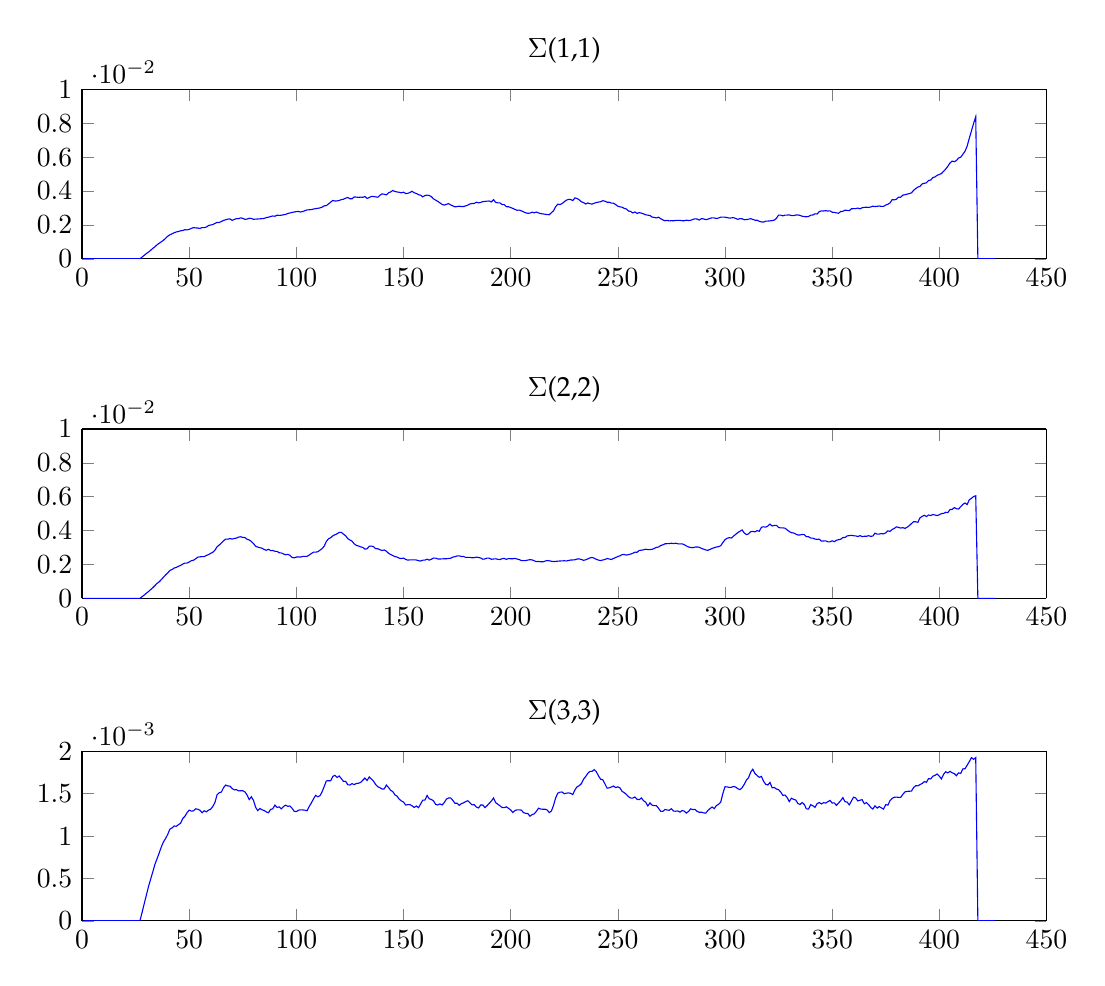
\begin{tikzpicture}

\begin{axis}[%
width=4.822in,
height=0.847in,
at={(0.809in,3.31in)},
scale only axis,
separate axis lines,
every outer x axis line/.append style={black},
every x tick label/.append style={font=\color{black}},
xmin=0,
xmax=450,
every outer y axis line/.append style={black},
every y tick label/.append style={font=\color{black}},
ymin=0,
ymax=0.01,
axis background/.style={fill=white},
title={$\Sigma\text{(1,1)}$}
]
\addplot [color=blue,solid,forget plot]
  table[row sep=crcr]{%
1	0\\
2	0\\
3	0\\
4	0\\
5	0\\
6	0\\
7	0\\
8	0\\
9	0\\
10	0\\
11	0\\
12	0\\
13	0\\
14	0\\
15	0\\
16	0\\
17	0\\
18	0\\
19	0\\
20	1.10668068063497e-28\\
21	6.1269188077788e-29\\
22	1.21154341531275e-27\\
23	2.16417281386742e-27\\
24	6.14431246491431e-27\\
25	6.28434927927247e-27\\
26	6.73213425124081e-27\\
27	5.07990940394863e-28\\
28	0.000100848759663641\\
29	0.00020187458630563\\
30	0.000305214346819941\\
31	0.000398660148707806\\
32	0.000499726900089777\\
33	0.00061192158000982\\
34	0.000708930345163692\\
35	0.000827918770452437\\
36	0.00091868681683618\\
37	0.00100197044500345\\
38	0.00109437218641779\\
39	0.00121342497173134\\
40	0.00133195545626767\\
41	0.00141823104363627\\
42	0.00147534380135983\\
43	0.00153731462564227\\
44	0.00158465558470437\\
45	0.00161161690715752\\
46	0.00165206093191761\\
47	0.00166981777931582\\
48	0.00171804000766001\\
49	0.00170631699294439\\
50	0.00173851789157291\\
51	0.00179223648974585\\
52	0.00183936471620231\\
53	0.00182310648097971\\
54	0.00181498429416863\\
55	0.00178917674870309\\
56	0.00183994667323329\\
57	0.00183880120246031\\
58	0.00187236753121147\\
59	0.00196158996028609\\
60	0.00199432071828742\\
61	0.00201714297453399\\
62	0.00208460294759297\\
63	0.00214652306975963\\
64	0.00214265193310957\\
65	0.00219868508884968\\
66	0.00226426280496353\\
67	0.00230408818126919\\
68	0.0023408784342245\\
69	0.00235403209879532\\
70	0.00226827797836073\\
71	0.00232033446250976\\
72	0.00236911589104423\\
73	0.002365903289477\\
74	0.0024171892358195\\
75	0.00238586112474731\\
76	0.00232927765645765\\
77	0.00234149551120929\\
78	0.00239405169022441\\
79	0.00237777287871326\\
80	0.00233320489064618\\
81	0.00234151787734478\\
82	0.00234948408204308\\
83	0.00235944604561368\\
84	0.0023699385354519\\
85	0.00238191501583074\\
86	0.00243532228243168\\
87	0.00245332531953899\\
88	0.00249787718767231\\
89	0.00252682422052829\\
90	0.00251095190728026\\
91	0.00257744077134686\\
92	0.00255862456799322\\
93	0.00257329973758199\\
94	0.0025964145974395\\
95	0.00261983730191888\\
96	0.00267576439870782\\
97	0.00270363472710814\\
98	0.00273540525674294\\
99	0.00276067516512187\\
100	0.00278631074366188\\
101	0.00279233327817584\\
102	0.00276275022841953\\
103	0.00278865765676907\\
104	0.00284144709007201\\
105	0.00288280220871039\\
106	0.00289431325542503\\
107	0.0029046595732406\\
108	0.00293621878515766\\
109	0.00296127253800892\\
110	0.00298144365824422\\
111	0.00300197408752758\\
112	0.00304853956320662\\
113	0.00312738246397327\\
114	0.00313752844144664\\
115	0.00323995894700459\\
116	0.00334426486425147\\
117	0.00344330092484347\\
118	0.00340927013385469\\
119	0.00341733958671464\\
120	0.00344580903204775\\
121	0.00349192413918856\\
122	0.00351637763763639\\
123	0.00358221663619034\\
124	0.00361705091063439\\
125	0.0035436681607256\\
126	0.00354119616168422\\
127	0.0036529348867921\\
128	0.00364123727188945\\
129	0.003626852367933\\
130	0.00363783043905127\\
131	0.00363251396216881\\
132	0.00367344457001959\\
133	0.00356800291719922\\
134	0.00361325887447694\\
135	0.00368506220515819\\
136	0.00367453225551926\\
137	0.00365665373707\\
138	0.00363466810309075\\
139	0.0037509007557095\\
140	0.00383212035603466\\
141	0.00380973917925498\\
142	0.0037728854319384\\
143	0.00389388972526819\\
144	0.00394511636830079\\
145	0.00403256666484179\\
146	0.00397428300900783\\
147	0.00394277203690242\\
148	0.0039267521983077\\
149	0.00389409260409789\\
150	0.00393183027997855\\
151	0.00385070532229674\\
152	0.00386387169272818\\
153	0.00391435810966989\\
154	0.00398516930076559\\
155	0.00389521188821937\\
156	0.00385464520089499\\
157	0.00378587264207597\\
158	0.00374943798269655\\
159	0.00365622475233085\\
160	0.00373113035666882\\
161	0.00375880836109623\\
162	0.00373744149184959\\
163	0.00367190667563139\\
164	0.0035382154659741\\
165	0.00346171558808308\\
166	0.00339279018079965\\
167	0.00329994637304831\\
168	0.00320698079219232\\
169	0.00316911963246575\\
170	0.00321136256350379\\
171	0.00325581854841401\\
172	0.00318083539976905\\
173	0.00312403689446414\\
174	0.00306927534170966\\
175	0.00307801036982269\\
176	0.0031067814948014\\
177	0.00308267425073142\\
178	0.00308521063868562\\
179	0.00312071836267238\\
180	0.00316907108981676\\
181	0.00323735917622743\\
182	0.00326140044617571\\
183	0.0032669441160519\\
184	0.00334048681538286\\
185	0.00329794248103543\\
186	0.00332671759036052\\
187	0.00337396268442482\\
188	0.00338666859837515\\
189	0.00340301556506458\\
190	0.00341065571121403\\
191	0.00335540547875238\\
192	0.00349252741341112\\
193	0.00333132426594948\\
194	0.00330207179669148\\
195	0.0032985388514196\\
196	0.00320242889181633\\
197	0.00319601154911751\\
198	0.00307514549851362\\
199	0.00307477024042898\\
200	0.00302247293532463\\
201	0.00297537751101938\\
202	0.00291477690550335\\
203	0.00286461940120865\\
204	0.00287415118853271\\
205	0.0028301426446641\\
206	0.00277349706618181\\
207	0.00271072448634254\\
208	0.00268867243669324\\
209	0.00269340681839635\\
210	0.00275209560572301\\
211	0.00271741746342264\\
212	0.00275733382987517\\
213	0.00271144055892187\\
214	0.00266378446039729\\
215	0.00265237171957067\\
216	0.00262965062063816\\
217	0.00261164909910056\\
218	0.00260043668310072\\
219	0.00272049309242529\\
220	0.00283304822372427\\
221	0.00307734942174367\\
222	0.00322628078786898\\
223	0.00320004568578852\\
224	0.00326173375686092\\
225	0.00336393498011407\\
226	0.00345820530964664\\
227	0.00351023494096158\\
228	0.00349817005547822\\
229	0.00343877432271297\\
230	0.00359610133657647\\
231	0.00355797273417922\\
232	0.0034777240401972\\
233	0.00336273886208658\\
234	0.00331824633399705\\
235	0.0032336949960527\\
236	0.00329751175641192\\
237	0.00325012762354946\\
238	0.00322694639863512\\
239	0.00328326790187974\\
240	0.00331957731045358\\
241	0.00334860372720795\\
242	0.00336579111464971\\
243	0.0034328540094083\\
244	0.00339741840515641\\
245	0.00333921638153673\\
246	0.003335385397944\\
247	0.00328980350271625\\
248	0.00328045930314612\\
249	0.00320126414066233\\
250	0.00310218241601566\\
251	0.00306779083494196\\
252	0.00304420443128089\\
253	0.00297414233423904\\
254	0.00294143314650612\\
255	0.00281809131033094\\
256	0.00279642880777856\\
257	0.00270547362033571\\
258	0.00276381895253267\\
259	0.00267810717498941\\
260	0.00272767925454094\\
261	0.0026955688712623\\
262	0.00264957642035699\\
263	0.00259856800007769\\
264	0.00257361222452978\\
265	0.00255657640871781\\
266	0.00246215825353807\\
267	0.00244395477210011\\
268	0.00241164645240594\\
269	0.00245530732164177\\
270	0.00236710289468012\\
271	0.00229530405959478\\
272	0.00224568073416289\\
273	0.00226659077539502\\
274	0.00223464330375853\\
275	0.00225210003804218\\
276	0.00224238070355001\\
277	0.00226239299895728\\
278	0.00227047348998711\\
279	0.0022678346304781\\
280	0.00224832191366107\\
281	0.00224248960935349\\
282	0.00228144221268781\\
283	0.00225891346326784\\
284	0.00226779203284323\\
285	0.00232571324196953\\
286	0.00235590248557222\\
287	0.00234883423819427\\
288	0.00228787734448393\\
289	0.00236858726750108\\
290	0.00235776727640733\\
291	0.00231465683392346\\
292	0.00233598980586208\\
293	0.00238979528474089\\
294	0.00241612506176601\\
295	0.00241167162108977\\
296	0.00237699012969247\\
297	0.00240517524894465\\
298	0.00246111690188362\\
299	0.00245687120641529\\
300	0.00245554727911624\\
301	0.00243295940622249\\
302	0.00240148171280924\\
303	0.0024140663616195\\
304	0.00243143879798746\\
305	0.00237844958476717\\
306	0.00232819459928758\\
307	0.00237307907753375\\
308	0.00236189148596975\\
309	0.00230589615424601\\
310	0.00231493988663886\\
311	0.00233900216899811\\
312	0.00236657304854402\\
313	0.00232764349488959\\
314	0.00227842531811331\\
315	0.00227146495343276\\
316	0.00221412839590192\\
317	0.0021764469820796\\
318	0.00216589780628802\\
319	0.00222209450781776\\
320	0.00222598152870172\\
321	0.00223784271737126\\
322	0.00225659156987155\\
323	0.0022810933586937\\
324	0.00238604252196671\\
325	0.00258002512752241\\
326	0.00257839317942149\\
327	0.00253273937677315\\
328	0.00257676885317372\\
329	0.00257966222034914\\
330	0.00259304067974815\\
331	0.00255238637078959\\
332	0.0025514472362451\\
333	0.00258285827787676\\
334	0.00258995261429763\\
335	0.0025645178523464\\
336	0.00251067566123136\\
337	0.00249401033119698\\
338	0.00247790409138355\\
339	0.00249788883940928\\
340	0.00257434198523513\\
341	0.00258575158695108\\
342	0.00265603210934583\\
343	0.00264462156415792\\
344	0.00278446326520044\\
345	0.00282585908575521\\
346	0.00282289573351223\\
347	0.0028401094606798\\
348	0.00282000928241824\\
349	0.00283092890285192\\
350	0.00274998437542993\\
351	0.00274003754852565\\
352	0.00271131781225898\\
353	0.00268886344780581\\
354	0.00279143233929278\\
355	0.00280323697581848\\
356	0.00286998274023674\\
357	0.00285703282056481\\
358	0.00284092053650496\\
359	0.00295589296472323\\
360	0.00295744649833703\\
361	0.00296470154287788\\
362	0.00299412335421933\\
363	0.00295230576426795\\
364	0.00301133810426407\\
365	0.00303797344449657\\
366	0.00304132025756168\\
367	0.00303499572730093\\
368	0.00305693595326837\\
369	0.00310822968073136\\
370	0.00308137675693312\\
371	0.00309829259605997\\
372	0.00311597387892222\\
373	0.00309151746079285\\
374	0.00309520155722467\\
375	0.00316952145388568\\
376	0.00321903484475224\\
377	0.00329925077708536\\
378	0.00349103613942927\\
379	0.00347746133843664\\
380	0.00351660771752692\\
381	0.00363790133883498\\
382	0.00363399260403543\\
383	0.00375810841157792\\
384	0.00378019550220131\\
385	0.00381531438437427\\
386	0.00384959868468275\\
387	0.00388705878373685\\
388	0.00403860588816837\\
389	0.00414604309088629\\
390	0.0042334946587986\\
391	0.00427367079910944\\
392	0.00442306181322667\\
393	0.00445673700429629\\
394	0.00448589268786409\\
395	0.00462184171616086\\
396	0.00464834394488013\\
397	0.00479597851303637\\
398	0.00483192938404075\\
399	0.00492840165468948\\
400	0.00497465682900664\\
401	0.0050301619736226\\
402	0.00516281013157313\\
403	0.0052994938873196\\
404	0.00546464233796071\\
405	0.00565770158380136\\
406	0.00576519648909404\\
407	0.00573169884412423\\
408	0.00580283648877756\\
409	0.00594635015888821\\
410	0.00599745319912589\\
411	0.00617058143416695\\
412	0.00634555457321202\\
413	0.00665201162897187\\
414	0.00711568500770019\\
415	0.00754824961331814\\
416	0.00798618136175051\\
417	0.00838168466761682\\
418	0\\
419	8.59482111715421e-29\\
420	4.52065586738225e-28\\
421	5.69824097157236e-28\\
422	5.2058007742508e-28\\
423	1.15426823496841e-27\\
424	3.32046270707128e-27\\
425	1.33844130021813e-26\\
426	1.32562719207329e-26\\
};
\end{axis}

\begin{axis}[%
width=4.822in,
height=0.847in,
at={(0.809in,1.612in)},
scale only axis,
separate axis lines,
every outer x axis line/.append style={black},
every x tick label/.append style={font=\color{black}},
xmin=0,
xmax=450,
every outer y axis line/.append style={black},
every y tick label/.append style={font=\color{black}},
ymin=0,
ymax=0.01,
axis background/.style={fill=white},
title={$\Sigma\text{(2,2)}$}
]
\addplot [color=blue,solid,forget plot]
  table[row sep=crcr]{%
1	0\\
2	0\\
3	0\\
4	0\\
5	0\\
6	0\\
7	0\\
8	0\\
9	0\\
10	0\\
11	0\\
12	0\\
13	0\\
14	0\\
15	0\\
16	0\\
17	0\\
18	0\\
19	0\\
20	2.3092102757602e-31\\
21	3.44565267984446e-32\\
22	7.56912744955378e-31\\
23	1.74978076984088e-30\\
24	6.07704005843463e-30\\
25	3.31726457317823e-31\\
26	1.06904617200073e-30\\
27	5.7604983688661e-33\\
28	9.9706112770798e-05\\
29	0.000195264961901317\\
30	0.000302657841997122\\
31	0.000403140083555271\\
32	0.00051829659432825\\
33	0.000630224393405465\\
34	0.000753061453319728\\
35	0.000889588761697916\\
36	0.000976179111015932\\
37	0.001110031024608\\
38	0.00125017646731135\\
39	0.00138873757680387\\
40	0.00150979479602322\\
41	0.0016481467399085\\
42	0.00170400928396534\\
43	0.00179305297270795\\
44	0.00182790202676668\\
45	0.00189478946880596\\
46	0.00194497810609458\\
47	0.00202820008269657\\
48	0.00208224033899094\\
49	0.00208357650600246\\
50	0.00214745474228115\\
51	0.00222496606119348\\
52	0.00225243853589112\\
53	0.0023360365409956\\
54	0.00243288596155356\\
55	0.00245216652863957\\
56	0.00246858645113004\\
57	0.00246712412777587\\
58	0.00253511828966251\\
59	0.00258122615058212\\
60	0.00265780429982336\\
61	0.00272347404857537\\
62	0.0028423659542254\\
63	0.00304547311890563\\
64	0.00314782465076192\\
65	0.0032698934847379\\
66	0.00339737473162562\\
67	0.00350108165764746\\
68	0.00349381816107716\\
69	0.00353211737004792\\
70	0.0035020092601733\\
71	0.00353360769701727\\
72	0.00355544247024938\\
73	0.00361688865341291\\
74	0.00363794022178958\\
75	0.00360303739151165\\
76	0.00359140594527181\\
77	0.00349332738508309\\
78	0.00344930550098657\\
79	0.00336176116363055\\
80	0.00323854779682972\\
81	0.00307591618251345\\
82	0.00303127498366353\\
83	0.00299217628538033\\
84	0.00296100663902265\\
85	0.00288841280644674\\
86	0.00283865219161244\\
87	0.00290055828510472\\
88	0.00281892979223406\\
89	0.00282931775579293\\
90	0.00277961036784225\\
91	0.0027746785115651\\
92	0.00269414072519423\\
93	0.00268365942301006\\
94	0.00262127966336223\\
95	0.002576220549711\\
96	0.00259994826931097\\
97	0.00254387052982565\\
98	0.00241812919549748\\
99	0.00239283704734936\\
100	0.00244112122472041\\
101	0.00244775481621803\\
102	0.00243700696470546\\
103	0.00248091555193516\\
104	0.00247615170126388\\
105	0.00248183172696894\\
106	0.00255946216754186\\
107	0.00264930639126633\\
108	0.00272638216404524\\
109	0.0027305429792762\\
110	0.00274998690728484\\
111	0.00284309636369812\\
112	0.00293887166051347\\
113	0.00308285745581302\\
114	0.00335942662762876\\
115	0.00351724898962991\\
116	0.00357880020417161\\
117	0.00369253156340483\\
118	0.00375549352465571\\
119	0.00381358692416067\\
120	0.00389445764591422\\
121	0.00389604900819425\\
122	0.00378992290215619\\
123	0.00369579866579864\\
124	0.00352827373246085\\
125	0.00344671395140915\\
126	0.00337690448854643\\
127	0.00321730109195499\\
128	0.00313190468035931\\
129	0.00308890906856404\\
130	0.00304314152992045\\
131	0.00300688661547937\\
132	0.00291114719341054\\
133	0.00292340467326134\\
134	0.00307548364257663\\
135	0.00308950290906321\\
136	0.00305438130803266\\
137	0.00293619419997882\\
138	0.00293068496821192\\
139	0.00287200271735087\\
140	0.00282955633375852\\
141	0.00285829269471127\\
142	0.00278746640545434\\
143	0.00266462485274948\\
144	0.00258821366906306\\
145	0.00252644037984459\\
146	0.00246883414171643\\
147	0.00244005744020341\\
148	0.0023757220215848\\
149	0.00235010153607885\\
150	0.00237926101073597\\
151	0.00230322310177544\\
152	0.00225812243697355\\
153	0.00227322962455555\\
154	0.00227460371364749\\
155	0.00227694802835216\\
156	0.00226765936658114\\
157	0.00222593997947298\\
158	0.00220363815398156\\
159	0.00225766055065618\\
160	0.00225995378292404\\
161	0.0023125352988197\\
162	0.0022583829667902\\
163	0.00231217019899345\\
164	0.00238185811571108\\
165	0.0023729202529566\\
166	0.0023284583159521\\
167	0.00232545369819298\\
168	0.00233220064592596\\
169	0.00233919888782922\\
170	0.00233985819719473\\
171	0.00235679734898935\\
172	0.00236800329116648\\
173	0.00243787100235458\\
174	0.00246161400309037\\
175	0.00250443351809805\\
176	0.00250999567774871\\
177	0.00247312227055276\\
178	0.00247866689410863\\
179	0.00241691964593458\\
180	0.00242536754635025\\
181	0.00242202139110883\\
182	0.00239809540404968\\
183	0.0024047810593772\\
184	0.00243863367377085\\
185	0.00241484681024189\\
186	0.00238423645677218\\
187	0.00231257693651683\\
188	0.00232952772379446\\
189	0.0023778307825746\\
190	0.00237170936776238\\
191	0.00230654824128771\\
192	0.00232733862132599\\
193	0.00233658431451234\\
194	0.00230788530019295\\
195	0.00228994276805879\\
196	0.00234387563245129\\
197	0.00235784020423919\\
198	0.00230451211977211\\
199	0.00234771210514634\\
200	0.00234163028300735\\
201	0.00233596592582212\\
202	0.00236084623294768\\
203	0.0023216969304872\\
204	0.00229272557257355\\
205	0.00222947841904866\\
206	0.00223212337837299\\
207	0.00223128377534369\\
208	0.0022631263320157\\
209	0.00228463950739984\\
210	0.0022741239343279\\
211	0.00221818203430041\\
212	0.00217224400988498\\
213	0.00217931035104218\\
214	0.0021609813749552\\
215	0.00215937306593518\\
216	0.00219911469073678\\
217	0.00223421724864596\\
218	0.00222145307186885\\
219	0.00219131245059122\\
220	0.00217492595607537\\
221	0.0021853352430007\\
222	0.00219658899924706\\
223	0.00220938224197246\\
224	0.00221125884431765\\
225	0.00222284242840037\\
226	0.00220904961417307\\
227	0.00223631456765684\\
228	0.00226319694318526\\
229	0.00226937420401831\\
230	0.00228084047208922\\
231	0.00232319699211223\\
232	0.00233095742191942\\
233	0.00229527966186581\\
234	0.00224574073829022\\
235	0.00227857264234822\\
236	0.00233120180447494\\
237	0.00239059721322884\\
238	0.00241415915939175\\
239	0.00236996473779623\\
240	0.00230386632798661\\
241	0.00226031858693508\\
242	0.00222847536476012\\
243	0.00226795996155498\\
244	0.00229609255827098\\
245	0.00235489372372258\\
246	0.0023252145676533\\
247	0.00229486835196553\\
248	0.00235669593761166\\
249	0.00241343357390411\\
250	0.00247130709940302\\
251	0.00251129432960098\\
252	0.00258521853390262\\
253	0.00258943952560804\\
254	0.00255317043034723\\
255	0.00258701477499137\\
256	0.00261569381602568\\
257	0.00266474167481027\\
258	0.00272868829969381\\
259	0.00272146028902216\\
260	0.00283253859032342\\
261	0.00284317873351517\\
262	0.00287053114334781\\
263	0.00290188978715412\\
264	0.0028798639587608\\
265	0.00288055228316175\\
266	0.00289643293680445\\
267	0.00294905174464496\\
268	0.00301389157171348\\
269	0.00302715452730709\\
270	0.00312330397422029\\
271	0.00315910336899373\\
272	0.00322431875266177\\
273	0.00322924930027064\\
274	0.00323064168070766\\
275	0.00325873457078564\\
276	0.00323071136591582\\
277	0.00325966892431472\\
278	0.00322251603580097\\
279	0.00321318711078771\\
280	0.0032196893873097\\
281	0.00317167987845344\\
282	0.00309512546691343\\
283	0.00303294483271509\\
284	0.00300802973329726\\
285	0.00299166345312673\\
286	0.00302929382591735\\
287	0.00303570138826785\\
288	0.00301742010863037\\
289	0.00295505117839523\\
290	0.00290818363941257\\
291	0.00285982384431352\\
292	0.002837123233782\\
293	0.00288920328862201\\
294	0.00294807233697439\\
295	0.00299029940659347\\
296	0.00303410287777665\\
297	0.00305194519150872\\
298	0.00310972708048728\\
299	0.0032964556726566\\
300	0.00346136833407191\\
301	0.00354928384118447\\
302	0.00358488126525837\\
303	0.003561975798834\\
304	0.00367779350868468\\
305	0.00378127002167373\\
306	0.00388720290216018\\
307	0.00396445934544959\\
308	0.00403950043191575\\
309	0.00386108247025581\\
310	0.00376374225286592\\
311	0.00380625784352414\\
312	0.00394111004883109\\
313	0.00395509937028042\\
314	0.00392805100446453\\
315	0.00400133641774484\\
316	0.00395976213864897\\
317	0.00419860010570251\\
318	0.00422544015641185\\
319	0.00420415757598269\\
320	0.0042756260447922\\
321	0.00438656332995888\\
322	0.00427045940765805\\
323	0.00431285330144758\\
324	0.00431289132797253\\
325	0.0041868155656308\\
326	0.00415891649256709\\
327	0.00416186628365365\\
328	0.00414548218320255\\
329	0.00404478094513689\\
330	0.00394904939613886\\
331	0.00387736879529139\\
332	0.00386300653877788\\
333	0.00379732173417042\\
334	0.0037449876156864\\
335	0.00374414465402782\\
336	0.00377596243031467\\
337	0.0037601461021554\\
338	0.00364422151271013\\
339	0.00363973826078994\\
340	0.00356246272328352\\
341	0.00355374538510005\\
342	0.00350467261822647\\
343	0.00348273015103891\\
344	0.00349870422617835\\
345	0.00337945298657171\\
346	0.00338949327166686\\
347	0.00339529520410932\\
348	0.00333888106451753\\
349	0.00334027918310603\\
350	0.00339889679870949\\
351	0.00334667740122978\\
352	0.00343052242300892\\
353	0.0034642584103535\\
354	0.00349270633761521\\
355	0.00359122078594816\\
356	0.00359368192347755\\
357	0.00368873948826739\\
358	0.0037055021742321\\
359	0.00372382329111147\\
360	0.00369827565194334\\
361	0.00368896114877588\\
362	0.00364880138896306\\
363	0.00371150438425152\\
364	0.00364333427910132\\
365	0.0036666582262105\\
366	0.00366640129348994\\
367	0.00369895144776376\\
368	0.00366369542100663\\
369	0.00367980893194507\\
370	0.00385166228073988\\
371	0.00379125981297013\\
372	0.00379806748901771\\
373	0.00382335666031338\\
374	0.00380884546591918\\
375	0.00387004191230176\\
376	0.00398646242430437\\
377	0.00395330537772604\\
378	0.0040635479513641\\
379	0.00413016327025163\\
380	0.00422528825682075\\
381	0.00418720632412052\\
382	0.00415309375921787\\
383	0.00417624376685373\\
384	0.00413095988073406\\
385	0.00420282255245611\\
386	0.00429326361903746\\
387	0.00441636105790642\\
388	0.00452572949470859\\
389	0.00452311998558726\\
390	0.00448943839291785\\
391	0.0047533746644874\\
392	0.0048436515065178\\
393	0.00490257622303824\\
394	0.00483300549325316\\
395	0.00492312944767602\\
396	0.00489198333067738\\
397	0.00494982389003544\\
398	0.00492456934547167\\
399	0.00488698701401681\\
400	0.00493761899522503\\
401	0.00500470304373184\\
402	0.00501969436244894\\
403	0.00508172347060684\\
404	0.00506466769840807\\
405	0.00524724051860508\\
406	0.00524861406530765\\
407	0.00536040213244758\\
408	0.00529440837203149\\
409	0.00527200847254663\\
410	0.00541604507277243\\
411	0.00555130118675692\\
412	0.00563144729927447\\
413	0.00553815090040565\\
414	0.00582399302661987\\
415	0.00590824257405288\\
416	0.0060119094672407\\
417	0.00605715281419544\\
418	0\\
419	2.91088280939153e-31\\
420	8.20058716756694e-31\\
421	7.05430649061133e-30\\
422	4.43778637050524e-31\\
423	7.28507703986261e-31\\
424	7.91782033798578e-30\\
425	3.47146272210348e-30\\
426	8.49420047479519e-32\\
};
\end{axis}

\begin{axis}[%
width=4.822in,
height=0.847in,
at={(0.809in,0in)},
scale only axis,
separate axis lines,
every outer x axis line/.append style={black},
every x tick label/.append style={font=\color{black}},
xmin=0,
xmax=450,
every outer y axis line/.append style={black},
every y tick label/.append style={font=\color{black}},
ymin=0,
ymax=0.002,
axis background/.style={fill=white},
title={$\Sigma\text{(3,3)}$}
]
\addplot [color=blue,solid,forget plot]
  table[row sep=crcr]{%
1	0\\
2	0\\
3	0\\
4	0\\
5	0\\
6	0\\
7	0\\
8	0\\
9	0\\
10	0\\
11	0\\
12	0\\
13	0\\
14	0\\
15	0\\
16	0\\
17	0\\
18	0\\
19	0\\
20	1.7248535839131e-29\\
21	1.06370118190604e-31\\
22	2.76784112346234e-30\\
23	3.13115298114261e-32\\
24	1.72462907025259e-30\\
25	5.12096548873076e-35\\
26	4.44279729871901e-30\\
27	6.81895538115503e-31\\
28	9.6754161160143e-05\\
29	0.000199203365673765\\
30	0.000299806152315689\\
31	0.000403208800830536\\
32	0.000490283724806267\\
33	0.000575907031529369\\
34	0.000665539780286951\\
35	0.000731959078140335\\
36	0.000800034334701908\\
37	0.000872365582738991\\
38	0.000932074499517547\\
39	0.000972110181864041\\
40	0.0010215964353307\\
41	0.00108218939916819\\
42	0.00109647367839539\\
43	0.00111947447430318\\
44	0.00111559815320495\\
45	0.00113515870536039\\
46	0.00115224211143195\\
47	0.00120757881927716\\
48	0.00123340289242875\\
49	0.0012761707792227\\
50	0.00130666509103807\\
51	0.00129458709535377\\
52	0.0012975532555746\\
53	0.00132179407519462\\
54	0.00131734114049655\\
55	0.00130570929149467\\
56	0.00127573212231027\\
57	0.00129903417089321\\
58	0.00128592061881932\\
59	0.00130640921475655\\
60	0.00131710618613246\\
61	0.00134909121622021\\
62	0.00139580420987756\\
63	0.00148717668624035\\
64	0.00151142977211426\\
65	0.00151987126692867\\
66	0.00157026660614571\\
67	0.00160209280477698\\
68	0.00159169870077908\\
69	0.00159019406284468\\
70	0.00156287000211426\\
71	0.00154547201879725\\
72	0.00154847670973836\\
73	0.0015341753835482\\
74	0.00153517435948171\\
75	0.00153585471545436\\
76	0.00152176027045775\\
77	0.00148533875684316\\
78	0.0014311380805345\\
79	0.00146475970301018\\
80	0.00142174733901931\\
81	0.00134015761242633\\
82	0.00130016611276461\\
83	0.0013255428184455\\
84	0.00131030773020504\\
85	0.0013024266197457\\
86	0.00128485267482426\\
87	0.00127647015690003\\
88	0.00131496140986789\\
89	0.00132210355481093\\
90	0.00136593566145524\\
91	0.00133785161424463\\
92	0.00134503922090162\\
93	0.00132170603841747\\
94	0.00134839921650332\\
95	0.00136520428968119\\
96	0.00135163911024807\\
97	0.00135564293542188\\
98	0.00132886137726828\\
99	0.00129206828327547\\
100	0.00128955426013171\\
101	0.0013052585128418\\
102	0.00130991570672195\\
103	0.00130849676081887\\
104	0.00130590946919857\\
105	0.00129936972832147\\
106	0.0013507386769909\\
107	0.00139109213404748\\
108	0.00143965546460088\\
109	0.00148096330768914\\
110	0.00146428398498244\\
111	0.00147586135058393\\
112	0.00152164465639154\\
113	0.00158557225756186\\
114	0.00165171443338191\\
115	0.00165408533320084\\
116	0.00165259869069844\\
117	0.00170432941931576\\
118	0.00171714100719894\\
119	0.00169167719164948\\
120	0.00170953945129422\\
121	0.00167840771666489\\
122	0.00164567527601362\\
123	0.00164681635722947\\
124	0.00160600985742446\\
125	0.00160324713803425\\
126	0.0016195001247134\\
127	0.00160778147571387\\
128	0.0016205478776052\\
129	0.00162400448859259\\
130	0.00163381770169068\\
131	0.00165939601009028\\
132	0.0016852147883562\\
133	0.00165589770624522\\
134	0.0016979890936276\\
135	0.0016733481602648\\
136	0.00164868130539554\\
137	0.00160897071398567\\
138	0.00158327113456202\\
139	0.00157065072261171\\
140	0.00155631864410361\\
141	0.00155659827931927\\
142	0.00160220800657783\\
143	0.00157369798710519\\
144	0.0015401161184108\\
145	0.00152560782405799\\
146	0.00148618071603048\\
147	0.00147160447652702\\
148	0.00143591223622855\\
149	0.00141572051093514\\
150	0.00140078659832657\\
151	0.00136641525408019\\
152	0.0013710756899813\\
153	0.00137138087119164\\
154	0.00135674775378257\\
155	0.00133792195564667\\
156	0.00135456606494152\\
157	0.00133587200199145\\
158	0.00137964408404113\\
159	0.00142441754332339\\
160	0.00142537524220168\\
161	0.00147983716143466\\
162	0.00143996537219037\\
163	0.00143230112941062\\
164	0.0014156584793652\\
165	0.0013737215884038\\
166	0.00136741147589617\\
167	0.00138017437325064\\
168	0.00136691925905098\\
169	0.00139466847124538\\
170	0.00143622177820473\\
171	0.00145000914069281\\
172	0.00145057609314006\\
173	0.00142168580788672\\
174	0.00138821728963338\\
175	0.00138790663381407\\
176	0.00136231288529131\\
177	0.00138367704835762\\
178	0.00139223832435803\\
179	0.0014079183682643\\
180	0.00141713960655984\\
181	0.001392706004028\\
182	0.00136814822424203\\
183	0.00137132348426966\\
184	0.00134315301043828\\
185	0.00133203676061731\\
186	0.00136647854691084\\
187	0.00136677333566025\\
188	0.00133676669587801\\
189	0.00135888101062154\\
190	0.00138746932026493\\
191	0.00141371055492804\\
192	0.00144916746773423\\
193	0.00139507477175163\\
194	0.00137609969991234\\
195	0.00135762741416442\\
196	0.0013376450138119\\
197	0.00133544184549174\\
198	0.00134538899183968\\
199	0.0013278948148298\\
200	0.0013091104691996\\
201	0.00127875693129451\\
202	0.00130086346685084\\
203	0.00130970269202077\\
204	0.0013095444015853\\
205	0.00130663163760585\\
206	0.0012765789714709\\
207	0.00126833336525075\\
208	0.00126682995134327\\
209	0.00123489278357952\\
210	0.00125414314656448\\
211	0.00126197245268243\\
212	0.0012925972889928\\
213	0.00132914431316953\\
214	0.00131980906065558\\
215	0.00131680535586316\\
216	0.00131731962241018\\
217	0.00130869452495883\\
218	0.00127815265425514\\
219	0.00129553536655735\\
220	0.00136237699861485\\
221	0.00145179698206201\\
222	0.00150652896302659\\
223	0.00151835300182406\\
224	0.00152045929747656\\
225	0.0015001369373442\\
226	0.00150636144914755\\
227	0.00151009719791592\\
228	0.00150465015167448\\
229	0.0014905641328116\\
230	0.00154590465811734\\
231	0.00158252763351101\\
232	0.0015949141855519\\
233	0.00161928599338058\\
234	0.00167139001050856\\
235	0.00170328831842226\\
236	0.0017416232573165\\
237	0.0017640090905657\\
238	0.00176480205455367\\
239	0.00178437701395232\\
240	0.00175860859200957\\
241	0.00170946115725696\\
242	0.0016709918951745\\
243	0.00166477697663183\\
244	0.00161576588458791\\
245	0.00156541843282333\\
246	0.00156950935529478\\
247	0.00158005833894228\\
248	0.0015904903247624\\
249	0.00157291576959621\\
250	0.00158170919193619\\
251	0.00156909492502477\\
252	0.00152788077674173\\
253	0.00151322823798498\\
254	0.00149195980772453\\
255	0.00146560133736168\\
256	0.00144828452575641\\
257	0.00144909447638486\\
258	0.00146139399869194\\
259	0.00143364846936791\\
260	0.001430030190862\\
261	0.00145031535645255\\
262	0.00141716287833444\\
263	0.00140015128906996\\
264	0.00135609407760717\\
265	0.00139157636703767\\
266	0.0013647395718138\\
267	0.0013590189349497\\
268	0.00136023358939131\\
269	0.0013281855690177\\
270	0.00129272295297476\\
271	0.00129182933470074\\
272	0.00131429970130774\\
273	0.00130828157434357\\
274	0.00130460619070009\\
275	0.00132338472153236\\
276	0.00129550697914511\\
277	0.00129363640644468\\
278	0.00129704418672982\\
279	0.00128304903132924\\
280	0.00130203528231314\\
281	0.001294819164506\\
282	0.00127168491139671\\
283	0.00129101604832138\\
284	0.00132185443718305\\
285	0.00131222392237511\\
286	0.00131561521049188\\
287	0.00129212943608748\\
288	0.00128061286316809\\
289	0.00128212675199019\\
290	0.00127434977384608\\
291	0.00127062624499807\\
292	0.00130184346880718\\
293	0.00132473362223438\\
294	0.00134341161701352\\
295	0.00132465040639261\\
296	0.00136066128057749\\
297	0.00137488752219386\\
298	0.00139969895879529\\
299	0.0015011951259519\\
300	0.00158191820352571\\
301	0.00158175544983102\\
302	0.0015737909218546\\
303	0.00157657556933595\\
304	0.00158486691619836\\
305	0.001579424598812\\
306	0.00155855256943751\\
307	0.00154834165696951\\
308	0.00157069786300814\\
309	0.00161139162282846\\
310	0.00166239126732431\\
311	0.00168907042854469\\
312	0.00175548914838796\\
313	0.00178979307942135\\
314	0.00173913392411074\\
315	0.00171445368336991\\
316	0.00169360040596805\\
317	0.00170514791963997\\
318	0.00164677372063768\\
319	0.00161107178592035\\
320	0.00160325542194868\\
321	0.00163362258667397\\
322	0.00157013343295921\\
323	0.00157397487788268\\
324	0.00155525310825572\\
325	0.00154741291936274\\
326	0.00152074108372628\\
327	0.00148088333556611\\
328	0.00148463315373839\\
329	0.00145513437374005\\
330	0.00140755316311721\\
331	0.00144731402016348\\
332	0.00143425800228531\\
333	0.00142631182167544\\
334	0.001385451354293\\
335	0.00137314380176544\\
336	0.00139686511639915\\
337	0.0013731329451762\\
338	0.00132104174386456\\
339	0.00131974822974635\\
340	0.00137143088873766\\
341	0.00135837583771851\\
342	0.0013393449641975\\
343	0.00138393922637382\\
344	0.0013960941205437\\
345	0.00137961452437825\\
346	0.00139459175686399\\
347	0.00139009327664205\\
348	0.00140579357735372\\
349	0.00142114124156016\\
350	0.00139050189855333\\
351	0.00139235087312719\\
352	0.00136239676076297\\
353	0.00139024445684926\\
354	0.00141884921472232\\
355	0.00145392856129467\\
356	0.00140630771175426\\
357	0.0014018805807347\\
358	0.00136857132517151\\
359	0.00141415178650178\\
360	0.00145929930736208\\
361	0.00144950856072683\\
362	0.00141479316290101\\
363	0.00142391818649302\\
364	0.0014299681730081\\
365	0.00138167585021859\\
366	0.00139513660050896\\
367	0.00137191035648503\\
368	0.00133821569349987\\
369	0.00131897055191841\\
370	0.00135738346231888\\
371	0.00133066780814565\\
372	0.00134899169013819\\
373	0.00133222416141408\\
374	0.00131887493750953\\
375	0.00137183470817798\\
376	0.00136545995510369\\
377	0.00141777369896475\\
378	0.00144540022832247\\
379	0.00145793885465185\\
380	0.00146038929838889\\
381	0.00145643723860481\\
382	0.00145705494076315\\
383	0.00149308074793898\\
384	0.00152222196317531\\
385	0.00152768882881863\\
386	0.00152977080074006\\
387	0.00153059332456909\\
388	0.00157262031408844\\
389	0.00159487909938003\\
390	0.00159290877129429\\
391	0.00160818588959097\\
392	0.00162020301812051\\
393	0.00164319411439647\\
394	0.00163563238867733\\
395	0.00167909650030264\\
396	0.00167477072965262\\
397	0.00170704626614322\\
398	0.00171686975426624\\
399	0.00173350706164378\\
400	0.00170776753742311\\
401	0.00167517200538889\\
402	0.00172942100306521\\
403	0.00175933991051307\\
404	0.00174619704098874\\
405	0.00176414798548735\\
406	0.0017471000031526\\
407	0.00173844307770727\\
408	0.00171279740762133\\
409	0.00174658899010658\\
410	0.00173993029513177\\
411	0.00179426208885431\\
412	0.0017946582568181\\
413	0.00183688442614995\\
414	0.00187873163670551\\
415	0.00192651237344538\\
416	0.00190647366048052\\
417	0.0019268923479514\\
418	0\\
419	1.77974025190453e-30\\
420	1.04053955816241e-30\\
421	4.88780684846589e-31\\
422	1.14438765963041e-29\\
423	7.32408102163463e-30\\
424	2.97487702750939e-29\\
425	5.76469219977654e-30\\
426	1.21735760886223e-30\\
};
\end{axis}
\end{tikzpicture}%}
	\caption{Uncertainty of pose when the number of particles $M=1000$ (left) and $M=10000$ (right).}
	\label{fig:Tracking_Uncertainty_Map_2_M_1000_10000}
\end{figure}

\par In \texttt{map\_sym3.txt}, there are 4 landmarks thus resulting in 4 hypotheses. Increase the number of particles $M$ from $1000$ to $10000$ would making the hypotheses more reliable. When $M$ is small and particles are spread over a large state space, the main drawback observed is particle deprivation which would discard particles near the correct state during the re-sampling step.
\par The multinomial sampling is not so effective when it comes to preserving multiple hypotheses since the multinomial sampling introduces random value for each particles.
\par When modeling stronger measurement noises, the particles would spread over a larger state space, and more hypotheses are preserved with lower accuracy.

\break
\subsubsection{map\_sym3.txt + so\_sym3\_nk}
\par Figure \ref{fig:converge_Map_3_M_10000} illustrate the images just before and just after the convergence.
\begin{figure}[!ht]
	\centering
	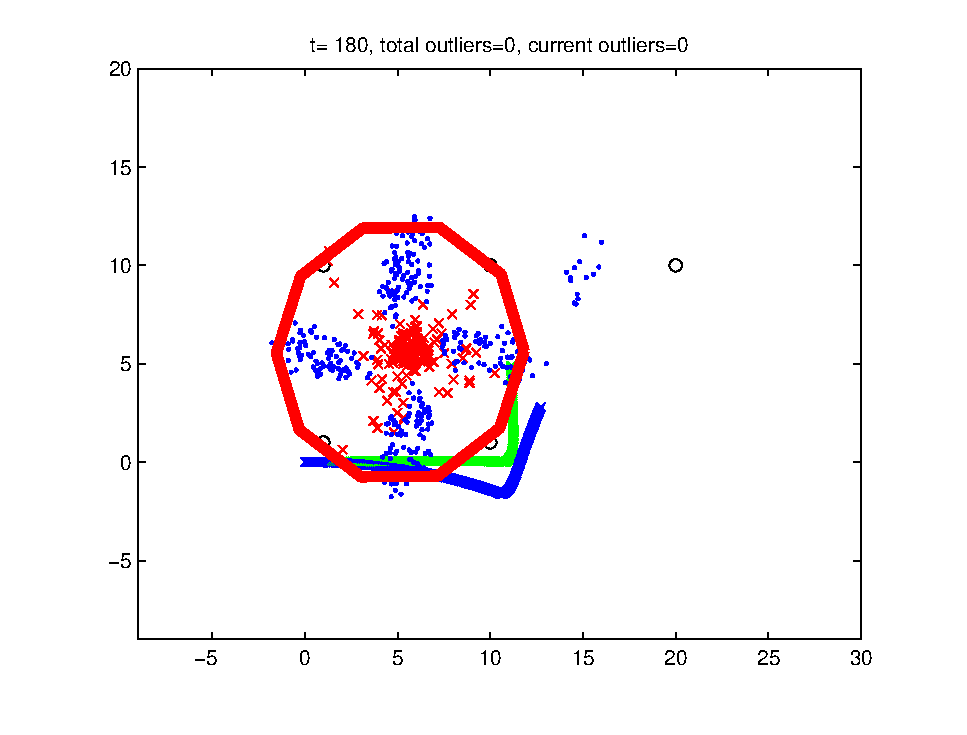
\includegraphics[scale=0.5]{./Figure/M=10000/2.eps}
	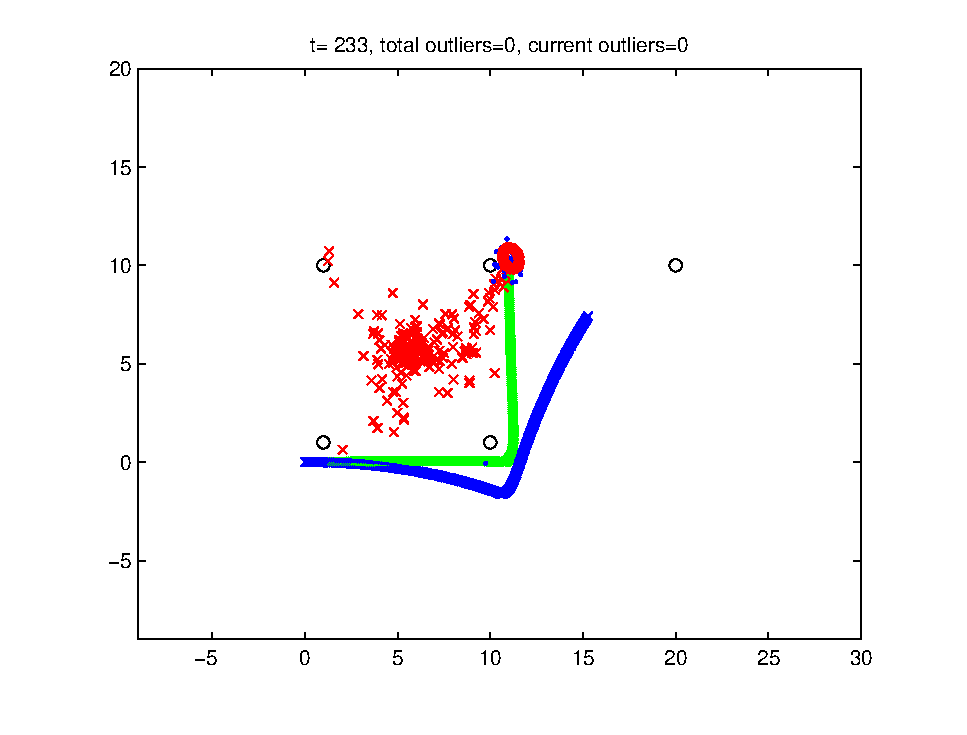
\includegraphics[scale=0.5]{./Figure/M=10000/4.eps}
	\caption{Time stamps of convergence.}
	\label{fig:converge_Map_3_M_10000}
\end{figure}

\end{document}